\documentclass[12pt,a4paper,twoside,openright,titlepage]{book}
\usepackage[utf8]{inputenc}
\usepackage[english,italian]{babel}
\usepackage[T1]{fontenc}
\usepackage[a4paper,top=3cm,bottom=2.5cm,left=4cm,right=3cm]{geometry}
\usepackage{graphicx}
\usepackage{booktabs}
\usepackage{indentfirst}
\usepackage{amsmath,amssymb,amsfonts} % Typical maths resource packages
\usepackage{numprint}
\usepackage[signatures,nowrite]{frontispiece} 
\graphicspath{{images/}}  % to include more paths: \graphicspath{{images_1/},{images_2/}}
%\DeclareGraphicsExtensions{.png, .pdf, .jpeg, .EPS} % image extensions
\usepackage{listings}
\lstset{language=C++,basicstyle=\small\ttfamily}
\usepackage[plainpages=false,pdfauthor={Piero Dalle Pezze},pdftitle={Master's Degree Thesis},pdftex]{hyperref}
\hypersetup{colorlinks=true,linkcolor=blue} % set colorlinks to true to enable colors (to remove for printing purposes)
\usepackage{url}
\usepackage[all]{hypcap}
\usepackage{subfigure}
\usepackage{color}
\usepackage{textcomp} % to use \textdegree
\usepackage{setspace}
\usepackage[small]{caption}
\usepackage{algorithm}
\usepackage{algorithmic}

\makeindex


% to remove titles in the empty page at the end of a chapter
\let\origcleardoublepage\cleardoublepage
\newcommand{\clearemptydoublepage}{
  \clearpage
  {\pagestyle{empty}\origcleardoublepage}
}
\let\cleardoublepage\clearemptydoublepage


% TO COMPILE run:
% makeindex -s thesis.ist -t thesis.glg -o thesis.gls thesis.glo
\usepackage[style=altlist]{glossaries}
\makeglossary

%\gls{linux} % displays name field of the linux entry (in this case "Linux")
%\useGlosentry{linux}{GNU/Linux} % displays "GNU/Linux"
%\GNU % displays "GNU's Not Unix (GNU)" the first time this is used
%\GNU % displays "GNU" all subsequent times
% NB: remember to use \GNU\ if want to retain the space after the acronym

% % TO COMPILE: makeindex -s thesis.ist -t thesis.glg -o thesis.gls thesis.glo
%% makeindex -s thesis.ist -t thesis.alg -o thesis.acr thesis.acn

% ACRONYMS
\newglossaryentry{ANN}{name={Artificial Neural Network (ANN)}, description={A mathematical model consisting of an interconnected group of artificial neurons. The information is processed by using a connectionist approach. In this thesis, only feed-forward neural networks are used. In feed-forward neural networks, the information moves in only one direction (forward) from the input, through the hidden to the output nodes without recurring cycles}}
\newglossaryentry{DSSP}{name={Dictionary of Secondary Structure in Proteins (DSSP)},description={The standard method for assigning secondary structure of a protein, given the 3D atomic coordinates}}
\newglossaryentry{CASP}{name={CASP},description={Critical Assessment of Techniques for Protein Structure Prediction. A community-wide experiment for protein structure prediction. It aims at establishing the current state of the art, identifying what progress has been made, and highlighting where future effort may be most productively focused}}
\newglossaryentry{FANN}{name={Fast Artificial Neural Network Library (FANN)},description={A free open source neural network library, which implements multilayer artificial neural networks in C programming language with support for both fully and sparsely connected networks. It includes a framework for easy handling of training data sets. \\
For more details see \href{http://leenissen.dk/fann/}{http://leenissen.dk/fann/}}}
\newglossaryentry{FM}{name={Free Modelling (FM)},description={A category of raw quality models, called free models,  obtained typically by using \emph{ab initio} or \emph{novel fold} prediction methods}}
\newglossaryentry{FRST}{name={Function of Rapdf, Solvation and Torsion potentials (FRST)},description={A MQAP method that predicts the model quality by using the pairwise, solvation, hydrogen bond, and torsion angle potentials. FRST was ranked 1st of 16 other MQAP methods in CASP-4, in 2004}}
\newglossaryentry{GDT}{name={Global Distance Test (GDT)},description={Also called Global Distance Test Total Score (GDT\_TS). A measure of similarity, adopted by CASP, between two protein structures with identical amino acid sequences but different tertiary structures. GDT\_TS is computed as $GDT\_TS = \frac{GDT\_P1 + GDT\_P2 + GDT\_P4 + GDT\_P8}{4}$ where $GDT\_Pn$ denotes percent of residues' carbon alpha atoms superimposed under distance cutoff less than $n$ \AA{}}}
\newglossaryentry{GIT}{name={Gauss Integrals Tuned (GIT)},description={A tool, developed by Peter R\o gen, for the description, comparison and classification of three-\-di\-men\-sio\-nal protein structures}}
\newglossaryentry{HQM}{name={High Quality Modelling (HQM)},description={A category of high quality models}}
\newglossaryentry{MQAP}{name={Model Quality Assessment Program (MQAP)},description={A program used to assess the quality of a protein model without any information about its corresponding native structure}}
\newglossaryentry{MSE}{name={Mean Squared Error (MSE)},description={A way to quantify the amount by which an estimator differs from the true value of the quantity being estimated. On details, it is defined as the mean difference between actual and predicted values: $MSE = \frac{1}{n}\sum_{i=1}^{n}(a_i - p_i)^2$ where $n$ is the number of samples, while $a_i$ and $p_i$ correspond to the true and predicted values for the $i$-th sample respectively. The MSE can also be written as the sum of the squared bias and variance of the estimator $f(x)$: $MSE(f(x)) = Bias^2(f(x)) + Var(f(x))$. The neural network performance can be improved if both the bias and variance are reduced. However, a neural network that fits closely the provided training examples has a low bias but high variance. On the other hand, a variance reduction leads to decrease the level of fitting the data. For this reason it needs a trade-off between bias and variance}}
\newglossaryentry{NMR}{name={Nuclear Magnetic Resonance (NMR)},description={NMR spectoscopy is an experimental method which allows to determine the structure of a protein in solution}}
\newglossaryentry{PDB}{name={Protein Data Bank (PDB)},description={A textual file format describing the three-\-di\-men\-sio\-nal protein structures stored in the Protein Data Bank (\href{http://www.rcsb.org/pdb}{http://www.rcsb.org/pdb}). It provides a rich description and annotation of protein properties like the protein name, the method used to obtain the pdb file, author names, annotations and the protein sequence. Then, for each atom, it reports its name, 3D atom coordinates, temperature factor and occupancy}}
\newglossaryentry{QMEAN}{name={Qualitative Model Energy ANalysis (QMEAN)},description={A single-model quality assessment program which defines the quality of a model as a weighed linear combination of statistical potentials}}
\newglossaryentry{RMSD}{name={Root Mean Square Deviation (RMSD)},description={A measure of the average distance between the backbones after having applied an optimal rigid body superposition}}
\newglossaryentry{SVM}{name={Support Vector Machine (SVM)},description={A supervised learning method used for classification and regression. In classification problems, input data are viewed as two sets of vectors in a n-dimensional space, and a SVM constructs a separating hyperplane in that space, maximizing the margin between the two data sets}}
\newglossaryentry{SVR}{name={Support Vector Regression (SVR)},description={A modified SVM used for regression problems. Differently from the classification problem in which the input data is categorized into two or more classes, in this case, each input data vector is associated to a real value (e.g. in $[0, 1]$) and the SVM tries to predict that value}}
\newglossaryentry{TBM}{name={Template-Based Modelling (TBM)},description={A category of medium quality models, called template-based models, obtained typically by using comparative modelling or fold recognition prediction methods}}
\newglossaryentry{VICTOR}{name={VIrtual Construction TOol for pRoteins (VICTOR)},description={A library of bioinformatics tools. Web Services using the VICTOR library are available at \href{http://protein.bio.unipd.it/services.shtml}{http://protein.bio.unipd.it/services.shtml}}}





% GLOSSARY
\newglossaryentry{amino_acid}{name={Amino Acid}, description={Also called residue. A body composed of a carboxyl group, an amino group and a side chain. In amino acids, bond lengths and bond angles between atoms are fixed. The carbon atom carrying the side chain is usually referred to as $C_\alpha$. The other atoms building the side chain are commonly called $\beta$, $\gamma$, $\delta$, $\varepsilon$ and $\zeta$ starting from the $\alpha$ carbon atom}}
\newglossaryentry{bias}{name={Bias}, description={The complexity restriction that the neural network architecture imposes on the degree of accurate fitting for the target function. The bias of an estimator $f(x) \approx E[y \arrowvert x]$ is $Bias(f(x)) = E_D[f(x)] - E[y \arrowvert x]$ where $D$ is the training data}}
\newglossaryentry{hydrogen_bond}{name={Hydrogen Bond}, description={The attractive force existing between the hydrogen covalently bonded to an electronegative atom of one molecule and an electronegative atom of a different molecule. Hydrogen bonds are a responsible component of the folding process}}
\newglossaryentry{model}{name={Model}, description={A predicted tertiary structure of a target sequence}}
\newglossaryentry{native_structure}{name={Native Structure}, description={The real tertiary structure of a protein. Native structures are found by X-Ray and NMR experimental methods}}
\newglossaryentry{target}{name={Target}, description={An amino acid sequence from which protein models are generated}}
\newglossaryentry{variance}{name={Variance}, description={The deviation of the neural network learning efficacy from one data sample to another sample that could be described by the same target function model. The variance of an estimator $f(x)$ is defined as $Var(f(x)) = E_D[(f(x) - E_D[f(x)])^2]$ where $D$ is the training data}}


% to customize header and footer of the page
\usepackage{fancyhdr}
\pagestyle{fancy}
\newcommand{\fncyblank}{\fancyhf{}}


%\title{Tesi di laurea Specialistica}
%\author{Piero Dalle Pezze} 
%\date{\today}


% figures: h, t (top), b (bottom), p (page). keep only t e b.

%hyphenation
\hyphenation{QMEAN-rannZ QMEAN-eannZ QMEAN-clust QMEAN-clustZ QMEAN-rann-clustZ QMEAN-eann-clustZ}

\begin{document}

	% page numbers and title will be located in the header of the page
 	\pagestyle{headings}
	\pagenumbering{roman}
	\begin{frontispiece}
	\end{frontispiece}
	
	% Setting the linespread (\usepackage{setspace})
	%\singlespacing
	\onehalfspacing
	%\doublespacing
	
	% the a short acknowledgment
	\begin{flushright}
		\cleardoublepage\null\vspace{\stretch{1}}
		\emph{Auf heimlich err\"othender Wange\\
		Leuchtet des Herzens Gl\"uhen}\\
		-- \textbf{S{\o}ren Kierkegaard}
		\vspace{\stretch{2}}\null
	\end{flushright}
	
	

\chapter*{Acknowledgments}
\addcontentsline{toc}{chapter}{Acknowledgments}	

I would like to thank my advisor Prof. Silvio C. E. Tosatto for giving me the opportunity to work at a renowned research center and supporting in the development of a complex method in a very competitive field such as protein model quality assessment. \\
I also thank my colleagues and friends in the laboratory where I spent a long time: Michele Vidotto, Maria Assunta Piano, Emanuela Leonardi, Gianpiero Zamperin, Francesco Sirocco.\\
I would like to thank Dr. Fabio Aiolli and Prof. Alessandro Sperduti for the courses in artificial intelligence carried out during the last two years which motivated me to choose a thesis in this field.\\
Last but not least, I thank my family for giving me the opportunity to study at the renowned University of Padua.
	
	% Abstract
	\newenvironment{abstract}
	{\cleardoublepage\fncyblank\null\vfill\begin{center}
	\bfseries\abstractname
	\end{center}}
	{\vfill\null}
	\selectlanguage{english}	
	\addcontentsline{toc}{chapter}{Abstract}		
	\begin{abstract}
The Model Quality Assessment Programs (MQAP) are assuming a crucial role in protein structure prediction. Clustering structure prediction methods have higher accuracy than individual structure prediction algorithms, although the first ones tend to fail if the best models are far from the center of the main cluster. In this work, a new hybrid clustering-based algorithm considers scores computed by another MQAP method to improve the accuracy. Two new individual methods whose scoring functions are based on neural networks are implemented for this purpose and used as support to the clustering assessment. Features from the QMEAN statistical potentials, Gauss invariants, hydrogen bonds and TAP score are used for these new methods. \\
CASP, which stands for Critical Assessment of Techniques for Protein Structure Prediction, is a community-wide experiment for protein structure prediction and aims to establish the current state of the art, identifying what progress has been made, and highlighting where future effort may be most productively focused. The clustering-based and individual methods developed in this work are tested on data from the CASP-4 and CASP-8 experiments, showing a significative improvement. The new hybrid clustering algorithm outperforms all other candidate methods at CASP-8, held in December 2008, achieving a global Pearson correlation between predicted quality score and GDT\_TS of $0.9485$ over $117$ targets for a total of $29,064$ models. Moreover, the individual methods based only on the QMEAN features outperform significatively the standard version of QMEAN.	
\end{abstract}
	
	
       % Italian abstract
       	\selectlanguage{italian}
	\addcontentsline{toc}{chapter}{Sommario}
	\begin{abstract}
I programmi per la valutazione della qualit\`a dei modelli (MQAP) stanno assumendo un ruolo cruciale nella predizione della struttura delle proteine. I metodi predittivi basati su clustering presentano un'accuratezza migliore rispetto a quelli basati su singolo modello, sebbene i primi tendano a fallire quando i modelli migliori sono molto distanti dal centro del cluster primario. In questo lavoro un nuovo algoritmo ibrido basato su clustering considera i punteggi computati da un altro MQAP per migliorare l'accuratezza. Due nuovi metodi individuali, le cui funzioni di valutazione sono basate su reti neurali, sono stati implementati a tale scopo e usati come supporto alla valutazione del clustering. Questi nuovi metodi sfruttano i potenziali statistici di QMEAN, gli integrali Gaussiani, i ponti di idrogeno e il TAP score. \\
Il CASP, che corrisponde a Critical Assessment of Techniques for Protein Structure Prediction, \`e un esperimento di interesse internazionale per la predizione delle strutture proteiche e si propone di stabilire l'attuale stato dell'arte, identificando il progresso ottenuto, e di indirizzare la ricerca futura. I metodi basati su clustering e quelli basati su reti neurali, sviluppati in questa tesi, sono stati testati sui dati provenienti dagli esperimenti del CASP-4 e del CASP-8, evidenziando un miglioramento significativo. Il nuovo algoritmo ibrido basato su clustering supera tutti gli altri metodi candidati al CASP-8, svolto a Dicembre del 2008, ottenendo una correlazione globale di Pearson tra il punteggio di qualit\`a predetto e il valore GDT\_TS di $0.9485$ su $117$ sequenze target per un totale di $29.064$ modelli. Inoltre, i metodi individuali basati solamente sui parametri utilizzati da QMEAN migliorano significativamente la versione standard di QMEAN.
	\end{abstract}
       	\selectlanguage{english}	
	
	\tableofcontents
	\listoffigures
	\listoftables
	\printglossary[nonumberlist]
	\addcontentsline{toc}{chapter}{Glossary}			
	
	\cleardoublepage
	\pagenumbering{arabic}
	
	\mainmatter
	

\chapter{Introduction}
\label{chap:introduction}

\section{Motivation}
\label{sec:motivation}
Bioinformatics may be defined as the study and analysis of biological material using computational methods. At least, two important areas of research exist: genomics and proteomics. Genomics comprises the study of genomes. The former aims to look at the discovery and understanding of the complete DNA sequence of organisms with the intent to gain a detailed genetic map. On the other hand, the interest for proteomics completes the knowledge about the next step in which the genetic information, once translated into amino acid sequence, determines the building blocks of life.\\
Proteins, which are the central topic of this work, are fundamental parts of organisms and participate in every process within cells. Many of them have enzymatic functions that catalyze biochemical reactions and are vital to the metabolism. Other proteins have comunicative functions like cell signaling, immune responses and cell cycle. Enzymes are proteins that catalyse biochemical reactions. The function of an enzyme relies on the structure of its active site, a cavity in the protein characterized by a specific shape and size that enable it to bind a certain substrate. A substrate may be another protein, a nucleic acid sequence or any other biochemical compound. Moreover, proteins transport and store other molecules such as oxygen, providing for mechanical support and immune protection. They allow the transmission of nerve impulses and are responsible for the growth control and cell differentiation. \\
Protein functions are determined by the three-\-di\-men\-sio\-nal structure of the protein and the physico-chemical properties of the amino acids at the active site. Therefore, knowledge about the structure of a protein is very important in order to discover its function, understand diseases and design new drugs. The number of known protein sequences is about two orders of magnitude higher than the number of experimentally solved protein structures and only a small subset of these has annotated function. New computational methods to predict the protein structure from its sequence are needed, because experimental methods for the determination of protein structures are time expensive, and fail for some types of proteins, such as membrane proteins. Given a target sequence for which the three-\-di\-men\-sio\-nal structure is desired, actual methods for protein structure prediction generate a huge amount of candidate models. In order to be able to discriminate good from bad protein models, a new class of computational methods has been developed to assess the quality of predicted models.

\section{Objectives}
\label{sec:objectives}
From the comparison of the most effective model quality assessment programs, it is known that clustering-based methods outperform those based on single-models. Methods belonging to the first category evaluate protein models by considering the ensemble, whereas the latter judge every model individually. These investigations suggest that future model quality assessment methods should consider a set of target models at once, while trying to minimize clustering drawbacks such as the loss of the best models which are far away from the core. \\
This work aims at the design and implementation of a new hybrid method for model quality assessment, based on clustering, that weights model scores by using a single-model method. The latter implements a neural network trained on features from the QMEAN statistical potentials, which is another single-model method. In more detail, the first goal is to demonstrate that a machine learning-based approach to the problem can improve the actual QMEAN performance. Different variants including both a single neural network and a neural system, are presented and discussed. The second objective comprises the exploration of new features besides those from QMEAN, again with the intention of outperforming the previous results. These new features consider hydrogen bonds, Gauss integrals and TAP score. Finally, the development of a method based on semi-clustering is treated. In order to improve the accuracy of the assessment, the latter takes into account the predicted model scores given by the previously cited single-model method, the model fraction that has been predicted and finally a categorization of the target sequence based on the predicted models.\\
CASP, which stands for Critical Assessment of Techniques for Protein Structure Prediction, is a community-wide experiment for protein structure prediction. It aims to establish the current state of the art, identifying what progress has been made, and highlighting where future effort may be most productively focused. The clustering-based and individual methods developed in this work are tested on data from the CASP-4 and CASP-8 experiments, showing a significative improvement. The new clustering-based algorithm outperforms all other methods participating in CASP-8, held in December 2008, achieving a global Pearson correlation between predicted quality score and GDT\_TS of $0.9485$ over $117$ targets for a total of $29,064$ models. In detail, the improvement with respect to ModFOLDclust, which is the best participating method and currently the best MQAP in the world, is of $\approx 1\%$ of global correlation. Also, it outperforms the QMEAN clustering-based version by $\approx 1.8\%$. The individual methods based only on the QMEAN features significatively outperform the standard version of QMEAN between $\approx 3\%$ and $\approx 6\%$ of Pearson’s correlation. Results on the CASP-4 test set are consistent with those in CASP-8.


\section{Outline}
\label{sec:outline}
This thesis is presented in four chapters. The first chapter contains a brief introduction to the performed work. The second chapter provides a more detailed discussion about protein structure and protein structure prediction with the aim to introduce the reader to the problem of model quality assessment. Beginning with the description of proteins, an overview of experimental and computational methods for the determination of three-\-di\-men\-sio\-nal protein structure is presented. A wide presentation on the state of the art for the model quality assessment programs is treated.\\
The third chapter describes the choices, design and implementation of the proposed methods. Starting with the description of QMEAN drawbacks, it discusses the single-model and the clustering-based methods, concluding with the new introduced features.\\
The fourth chapter presents the results achieved by the implemented methods on two test sets and provides a benchmark against the best currently available model quality assessment programs. An exhaustive series of plots is also reported with the motivation to illustrate details where methods fail or achieve good performances. Finally, a conclusive chapter is provided in order to summarize the developed work and define new possible research directions.\\
Two appendices comprising the ideas underlying force fields, statistical potentials and the mathematical theory of Gauss integrals are given as well.

\cleardoublepage




	
\chapter{Protein Structure and Prediction}
\label{chap:protein_structure_and_prediction}

\section{Protein Structure}
\label{sec:protein_structure}
Twenty different \glslink{amino_acid}{amino acids}, also called residues, constitute the building blocks of proteins. Amino acids are linked in proteins by the formation of peptide bonds between amino ($NH_2$) and carboxyl ($COOH$) groups of two adjacent residues as shown in Figure \ref{fig:peptide_bond_formation}. The unique physical and chemical properties that distinguish amino acids are determined by the $R$-group. The polypeptide chain forming the protein is also referred to as backbone. In each polypeptide chain, the $N$-terminus is the end of a polypeptide chain terminated by an amino acid with a free amine group. The $C$-terminus is the end of the backbone terminated by a free carboxyl group. By convention, peptide sequences are written from the $N$-terminus (left) to the $C$-terminus (right). A review concerning protein synthesis can be found in \cite{Lengyel1969}.
\begin{figure}[tb]
	\begin{center}
		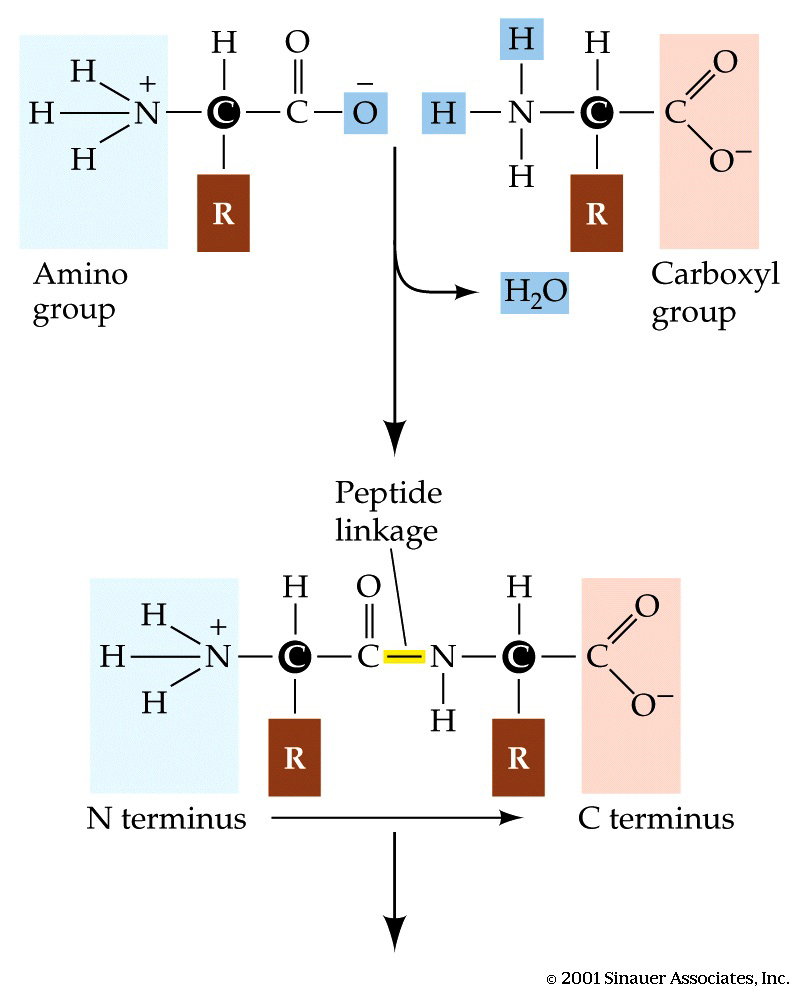
\includegraphics[scale=0.60]{peptide_bond_formation}
		\caption[Peptide bond formation]{Example of peptide bond formation. The carboxyl group ($COOH$) of the first residue binds with the amine group ($NH_2$) of the second residue, forming a peptide bond and a water molecule. The R-group is the group that distinguish an amino acid from the others.}
		\label{fig:peptide_bond_formation}
	\end{center}
\end{figure}
The backbone dihedral angles (or torsion angles) of proteins are called $\phi$ and $\psi$. The former involves the atoms $N-C_\alpha$, the latter the atoms $C_\alpha-C\ '$, as illustrated in Figure \ref{fig:dihedral_angles}. The Ramachandran plot, reported in Figure \ref{fig:ramachandran_plot}, shows all possible conformations of the angles $\phi$ and $\psi$ with the aim to analyze atom collisions by considering the van der Waals radius. Ramachandran \cite{Ramachandran1963} was the first to calculate which $\phi$ and $\psi$ angles are allowed. He modelled the permitted angles for a tripeptide, assuming the atoms were hard spheres. The allowed angles depended in part on the limiting distance chosen for interatomic contacts. The plot shows the allowed regions in red. The yellow zone describes the stable conformations, while the white zone represents collision conformations. For each residue, a specific Ramachandran plot can be defined.
There exist four levels of protein structure which refer to four distinct conceptual aspects:\\

\begin{description}
\item[Primary Structure.] The linear sequence of amino acids, encoded by the nucleotide sequence of the gene. 
\item[Secondary Structure.] The ordered array of amino acids in a protein confer regular conformational forms upon that protein. The secondary structure refers to those local structural patterns of the protein backbone.  Common elements of secondary structure are $\alpha$-helices, $\beta$-sheets and coil/loop. The $\alpha$-helix is a right or left handed coiled conformation generating a spring. The $\beta$-sheets is made of $\beta$-strands connected laterally by three or more \glslink{hydrogen_bond}{hydrogen bonds}.
\item[Tertiary Structure.] It describes the complete three-\-di\-men\-sio\-nal conformation of the protein. Figure \ref{fig:tertiary_structure_1LM8_sticks} shows an example of tertiary structure.
\item[Quaternary Structure.] It represents the arrangement of two or more different polypeptide chains forming a macromolecular complex.
\end{description}

\begin{figure}[tb]
	\begin{center}
		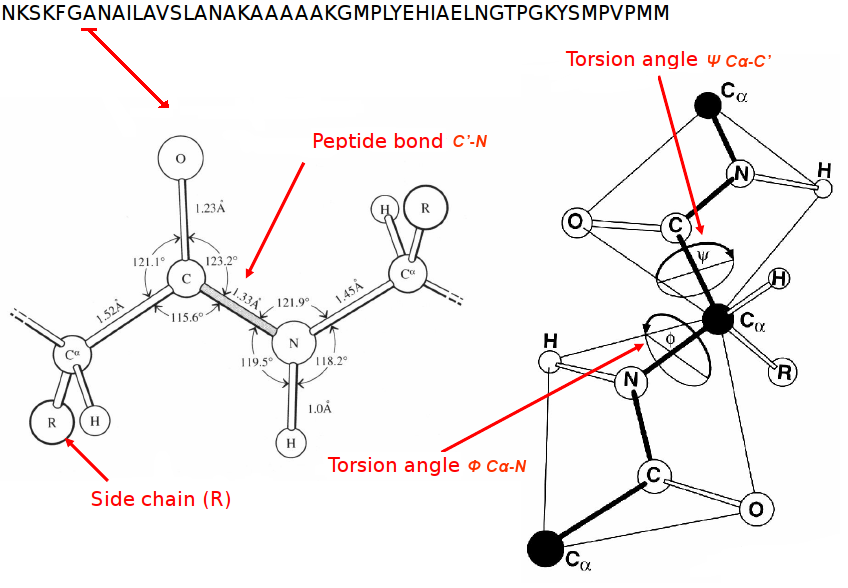
\includegraphics[scale=0.50]{dihedral_angles}
		\caption[Dihedral angles in polypeptides]{Dihedral angles in polypeptides.}		
		\label{fig:dihedral_angles}
	\end{center}
\end{figure}
\begin{figure}[tb]
	\begin{center}
		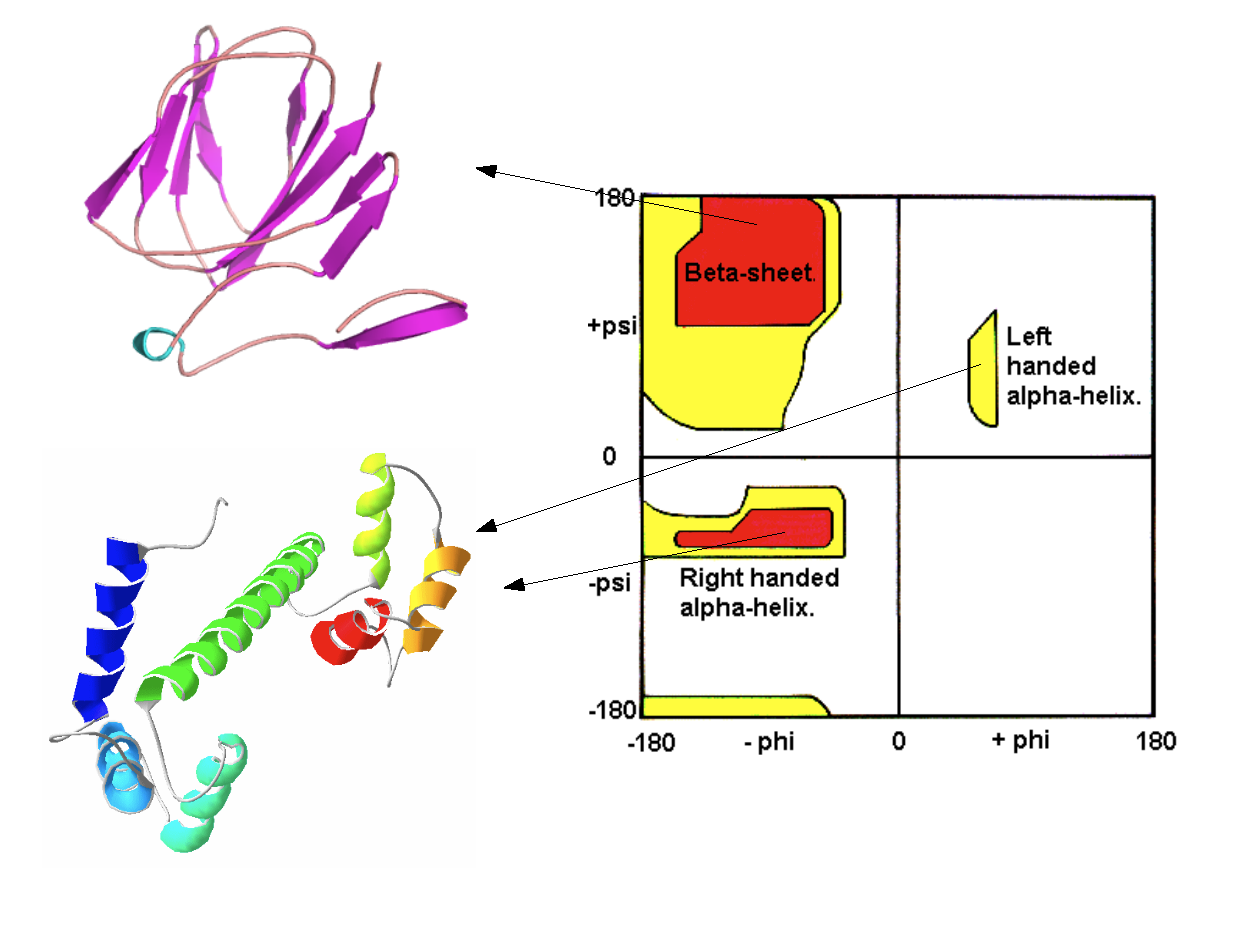
\includegraphics[scale=0.50]{ramachandran_plot}
		\caption[The Ramachandran plot]{The Ramachandran plot.}
		\label{fig:ramachandran_plot}
	\end{center}
\end{figure}
 \begin{figure}[tb]
	\begin{center}
		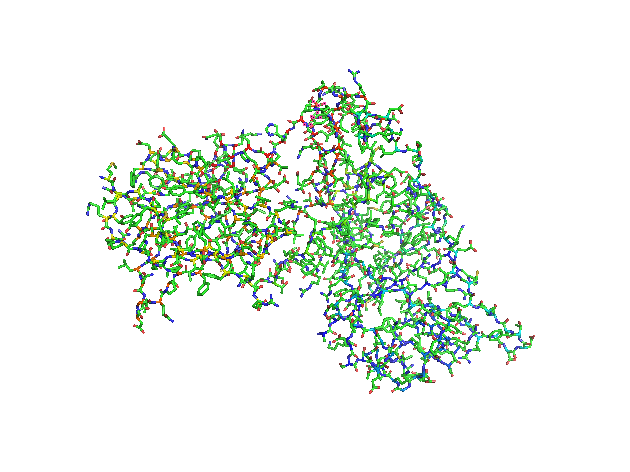
\includegraphics[scale=0.60]{1LM8_sticks}
		\caption[Tertiary structure of the protein 1LM8]{Example of the tertiary structure of the protein 1LM8.}
		\label{fig:tertiary_structure_1LM8_sticks}
	\end{center}
\end{figure}


\subsection{Sequence-Structure Relationship}
\label{subsec:sequence_structure_relationship}
Anfinsen's dogma \cite{Anfinsen1973aa} establishes that the primary sequence exclusively determines the 3-dimensional structure of a protein. Anfinsen demonstrated that the leading force for the folding process is the gradient of free energy and that the protein \glslink{native_structure}{native structure} is in its free energy minimum. Folding represents the physical process in which a polypeptide chain, such as a protein or a domain, changes state assuming its characteristic three-\-di\-men\-sio\-nal structure \cite{Lindorff-Larsen2005aa}. The folding process is still an unsolved problem \cite{Rose2006aa}. In the late 1960's, Levinthal showed that the search of all possible conformations of a polypeptide chain has exponential complexity, whereas the observed folding time is of microseconds to minutes in nature. This fact, known as Levinthal's paradox \cite{Levinthal1968aa}, demonstrates that an intensive, purely random search of the native conformation cannot succeed. Thus, he affirmed that proteins fold by following specific folding pathways.\\
Nowadays, the pathway concept based on a defined series of discrete intermediates is replaced by the concept of the energy landscape in which a multiplicity of parallel routes fall down a folding funnel. Figure \ref{fig:energy_landscape2} illustrates the funnel-like energy landscape.  The energy landscape is potentially rough due to kinetic traps and energy barriers.
\begin{figure}[tb]
	\begin{center}
		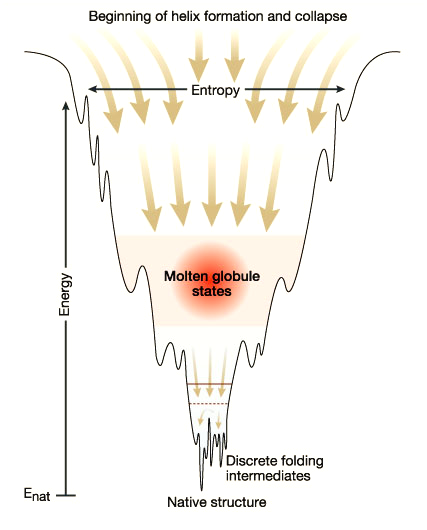
\includegraphics[scale=0.50]{energy_landscape2}
		\caption[Energy landscape for protein folding]{Energy landscape for protein folding. Protein folding does not follow a single, specific pathway, rather it follows a funnel of declining energy in which it can adopt many folding routes and still reach the native structure conformation.}
		\label{fig:energy_landscape2}
	\end{center}
\end{figure}
Often folding involves first the establishment of regular secondary and supersecondary structures, particularly $\alpha$-helices and $\beta$-sheets, and afterwards the subunits are assembled further down the folding funnel forming the known tertiary structure. The regular $\alpha$-helix and $\beta$-sheet structures fold rapidly because they are stabilized by intramolecular hydrogen bonds. The essential characteristic of folding, however, is that the amino acid sequence of each protein contains the needed information that specifies both the native structure and the pathway to reach that state. Folding is a spontaneous process independent of energy inputs. The passage to the folded state is mainly guided by hydrophobic interactions, formation of intramolecular hydrogen bonds, and van der Waals forces, and is opposed by conformational entropy \cite{Sippl1996aa}.\\
It is known that the protein function depends on the structure and this is defined by the sequence. However, prediction of protein structure from scratch solely based on physical principles currently does not achieve good results. Most current methods for protein structure prediction take into account knowledge from experimentally solved structures based on the fact that structure is more conserved than sequence.
Sequence similarity is commonly referred to as pairwise sequence identity achieved in an alignment. A pairwise alignment is a way of arranging two sequences in order to identify regions of similarity that may be a consequence of functional, structural, or evolutionary relationships between the sequences. Gaps, called also indels and denoted by ``-'', define missing residues in one or two sequences. Sequence identity describes the number of identical residues in two sequences divided by the length of the shorter sequence. After computing the sequence alignment and achieving an optimal structural superposition, the structural similarity is calculated by measuring the \gls{RMSD} between corresponding atoms of the two proteins.


\subsection{Experimental Methods}
\label{subsec:experimental_methods}
To characterize protein structures at atomic resolution, two experimental methods are usually adopted: X-ray crystallography and NMR-spectroscopy. In the Protein Data Bank (see \S~\ref{subsec:the_protein_data_bank_and_structural_genomics}), about $85\%$ of the reported protein structures are obtained by X-ray diffraction, while the remaining ones are found by NMR-spectroscopy.\\
The technique of X-ray crystallography has three basic steps. The first and often most difficult step is the production of an adequate crystal. The crystal should be sufficiently large, pure in composition and regular in structure, with no significant internal imperfections. Then, the crystal is irradiated with monochromatic X-rays, producing a diffraction pattern which is specific for the given protein structure. X-rays are waves that behave analogously to visible light on a larger scale, producing interference when scattered at the crystal. X-rays irradiating a crystal from a single direction are diffracted, which results in an interference pattern. The directions of these scattered X-rays, called reflections, depend only on the crystal lattice and not on the structure of the molecule. In this way, it is possible to collect reflections from all planes in the crystal, using a computer-guided diffractometer. The intensity of the collected reflections corresponds to the amplitudes of the molecular shape in Fourier space. Using the amplitude and the phases, the structure of the protein can be reconstructed by a Fourier transform. Unfortunately, the phase information cannot be measured by the diffractometer and additional information is needed in order to estimate the phases. A Fourier transform describes an image of the protein crystal in form of an electron density map. To place the atoms of the protein structure, the map needs to be interpreted. Because resolution for proteins is not always good enough, a further step to refine the obtained model, is required. Information about standard geometries for bond lengths and angles are used when fitting the model atoms to the electron density map. The final model is achieved by an iterative refinement of the structure. The resolution, measured in Angstrom (\AA{}), defines the accuracy of the obtained model. \\
\gls{NMR} spectroscopy is an alternative method for determining the structure of a protein in solution. The advantage with respect to X-ray crystallography is that proteins in solution are in their natural environment. However, the resolution of NMR structures is lower. The solution is exposed to a powerful magnetic field which causes the spin of the nuclei to be oriented in direction by the external field. The spin is the angular momentum of the atomic nuclei. Then, an additional magnetic field is used in order to switch the atom nuclei spin orientation. In this way the frequency, also called resonance frequency, can be measured. The resonance frequency differs for atoms depending on their chemical environment. Measuring the magnetic interaction between nuclear spins, distances of atoms close in space can be deduced. Given a sufficient number of distance constraints, these can be used to perform distance geometry calculations, with the aim to define the spatial arrangement of the polypeptide chain. NMR-spectroscopy usually produces up to $20$ or more models for a given protein, due to both the flexible character of proteins in solution and segments of the structure with few distance constraints. The more constraints are given and the closer the models become. \\
X-ray crystallography can solve structures of arbitrarily large molecules, whereas NMR-spectroscopy is restricted to relatively small molecules. X-ray crystallography defines more higher-resolution structures than NMR-spectroscopy, but is not able to capture well the molecular dynamics. Also, membrane proteins remain challenging to crystallize because they require detergents or other means to solubilize them in isolation, and these detergents often interfere with crystallization. For this kind of proteins, predictive methods are fundamental.


\subsection{The Protein Data Bank and Structural Genomics}
\label{subsec:the_protein_data_bank_and_structural_genomics}
The \gls{PDB} \cite{Berman2002aa} is a repository for the experimentally determined three-\-di\-men\-sio\-nal structural data of biological molecules, such as proteins and nucleic acids. Data submitted by biologists and biochemists from around the world are released into the public domain and can be accessed at no charge on the Web.\\
At present (March 2009) the PDB holds $52,170$ protein structures (see Table \ref{tab:pdb_current_holding_breakdown}). 
Although the number of known sequences recorded in the PDB grows exponentially, the number of newly discovered folds has decreased over the last years (see Figure \ref{fig:cewolf}). This can be due to the fact that, on one hand, some proteins, e.g. membrane proteins, are very difficult or impossible to determine with current methods; on the other hand, structural genomics initiatives have solved many of the missing folds over the last years.
Structural genomics consists in the determination of the one, two and three-\-di\-men\-sio\-nal structure of all proteins of a given organism, by experimental methods such as X-ray crystallography, NMR-spectroscopy or computational approaches \cite{Chance2004aa}. One of the major goals of the structural genomics initiative consists in high throughput protein structure determination. This allows to reduce research costs and increase the number of known structures. Targets for structural genomics are proteins with less than $30\%$ sequence identity to any structure in the PDB. Another important advantage of structural genomics is that the scientific community can immediately access to newly solved structures and relative documents.
\begin{figure}[tb]
	\begin{center}
		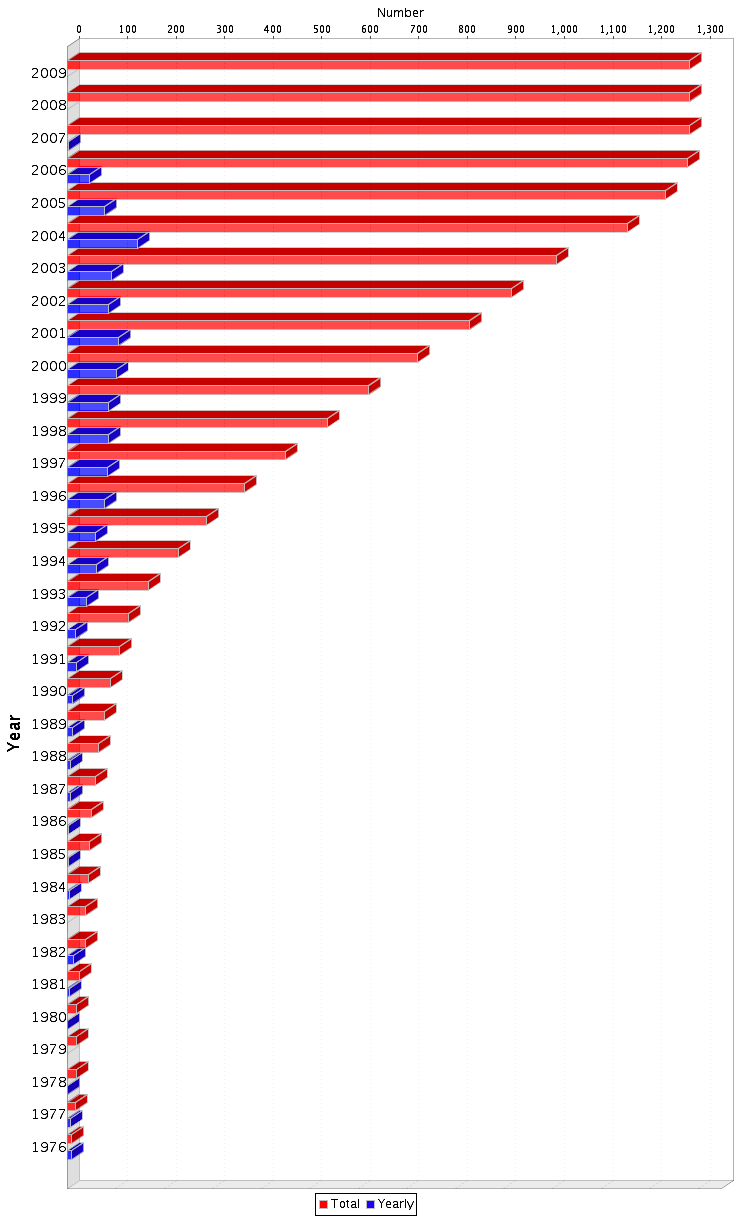
\includegraphics[width=12cm, height=15cm]{cewolf} 
		%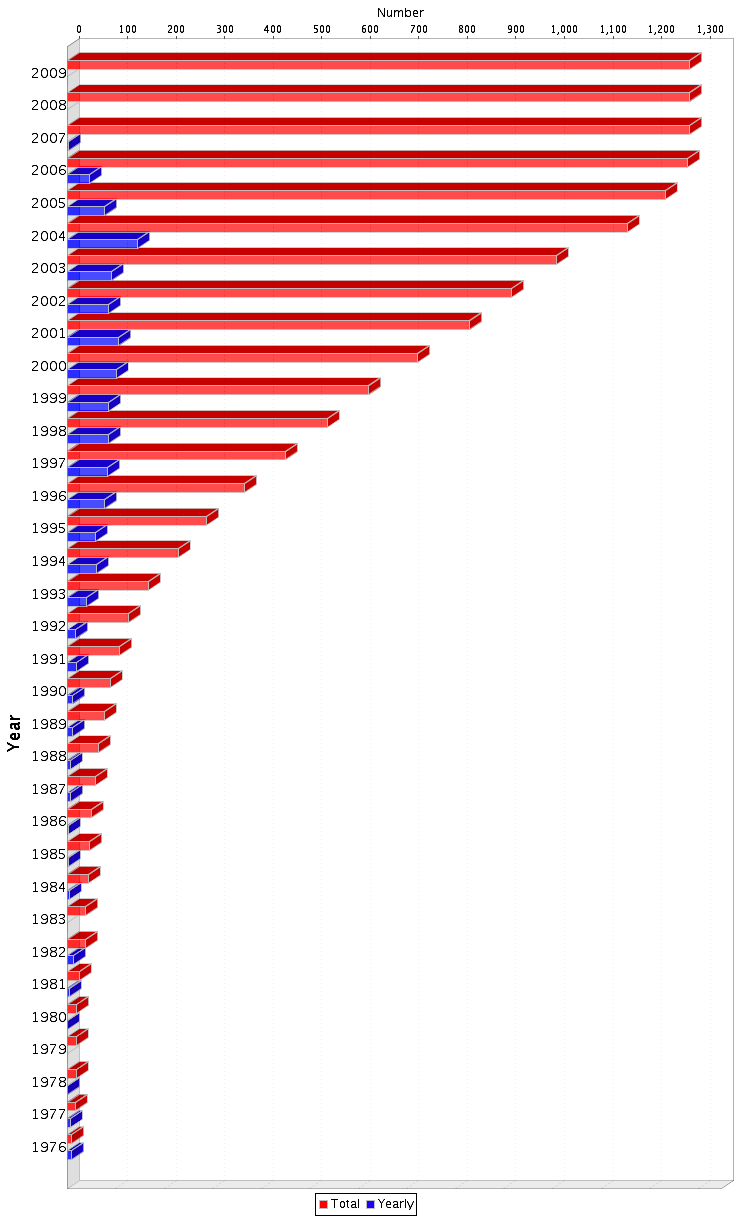
\includegraphics[scale=0.70]{cewolf}
		\caption[Growth in the number of unique folds available in the PDB, per year as define by SCOP]{Growth in the number of unique folds available in the PDB, per year as define by SCOP as of March 2009.}
		\label{fig:cewolf}
	\end{center}
\end{figure}
\begin{table}[tb]
\center
\begin{tabular}{lccc}
\toprule                % or \hline
\textbf{Exp. Method} & \textbf{Proteins} & \textbf{Nucleic Acids} & \textbf{Protein/Nucleic Acid} \\
\midrule                % or \hline
	X-ray		         &45149	&1088	&2064\\
	NMR 		         &6759	&831	&143\\
	Electron Microscopy &154		&16		&59\\
	Other			&108	&4		&4\\
	\textbf{Total} & \textbf{52170}	&\textbf{1939}	&\textbf{2270}\\
\bottomrule                % or \hline
\end{tabular}
\caption[Statistics of the PDB as of March 2009]{Statistics of the PDB as of March 2009.}
\label{tab:pdb_current_holding_breakdown}
\end{table}


\section{Protein Structure Prediction}
\label{sec:protein_structure_prediction}
The knowledge of the protein three-\-di\-men\-sio\-nal structure is important because it considerably simplifies functional annotation. Structural information is an important key from both theoretical and practical point of view. The number of known sequences (approximately $7.3$ million in UnitProt/TrEMBL\footnote{Source: \href{http://www.ebi.ac.uk/swissprot/sptr\_stats/index.html}{http://www.ebi.ac.uk/swissprot/sptr\_stats/index.html}}) is about two orders of magnitude greater than the fraction for which the structure is solved (see \S~\ref{subsec:the_protein_data_bank_and_structural_genomics}). 
Following the objective of structural genomics, new efficient and effective methods for protein structure prediction are needed, in order to close this existing gap.\\
Protein structure prediction means the prediction of tertiary structure of a protein using computational methods. The determination of the protein tertiary structure can be made in two different ways: the laws of physics and the theory of evolution. Methods that belong to the first approach are called \emph{ab initio}, while those that follow the second approach are called template-based methods.\\
\emph{Ab initio} or \emph{de novo} methods try to construct the structure of a protein based on physico-chemical properties of the amino acid chain. Theoretically, only the protein sequence is required. On the other hand, template-based methods consider structural information retrieved from known protein structures, called templates. These are used to build a model of the target sequence. From an evolutionary point of view, template-based methods are motived because structures are more conserved than sequences \cite{Chothia1986aa}. Also, they are justified by the biological reality in which there is a limited set of tertiary structural motifs to which most proteins belong \cite{Chothia1992aa}. Template-based modelling has been split into two groups: fold recognition and comparative (homology) modelling that differ on the way of template identification. The following sections deal with the different methods.\\
The choice of a good template is crucial in order to generate an accurate model for the target sequence. A good template  for a target sequence is a sequence of known structure that obtains a high similarity score when compared against the target. To highlight the importance of protein structure prediction and model quality assessment (see \ref{subsec:model_quality_assessment_programs}), it could be considered that, for instance, high to medium accuracy models, generated by homology modelling using a template with more than $30\%$ of sequence identity to the target, can be used as basis to understand interactions between residues capturing factors that arise a disease and thus be employed in drug design.


\subsection{Methods}
\label{subsec:methods}
\subsubsection{Comparative Modelling}
\label{subsubsec:comparative_modelling}
Comparative or homology modelling constructs the target structure by considering a homologous template structure. It is generally sufficient to have a sequence identity of about $30\%$ to establish a structural similarity between two proteins. This consideration is very important if related to the growth of the new experimentally solved protein structures, because it allows to increase the prediction of the structure for many known protein sequences.\\
Homology modelling refers to constructing a three-\-di\-men\-sio\-nal model of the \glslink{target}{target} protein from its amino acid sequence and an experimental three-\-di\-men\-sio\-nal structure of a related homologous protein (the template). As shown in Figure \ref{fig:comparative_modelling}, the comparative modelling framework is defined by the following steps: template identification and selection, target-template alignment, raw model building, loop modelling, side chain prediction, refinement and quality assessment. A short description of all steps is given below.\\
\begin{figure}[tb]
	\begin{center}
		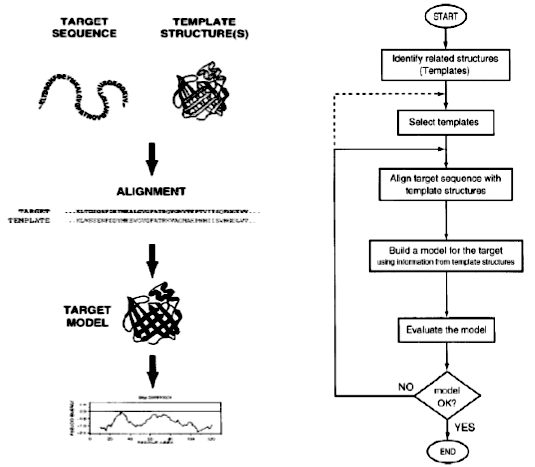
\includegraphics[scale=0.70]{comparative_modelling}
		\caption[The comparative modelling framework]{The comparative modelling framework.}
		\label{fig:comparative_modelling}
	\end{center}
\end{figure}
Comparative modelling requires at least one sequence of known three-\-di\-men\-sio\-nal structure with significant similarity to the target sequence. In order to determine if a modelling request can be carried out, the target sequence is compared with a database of sequences derived from the PDB, using programs such as FASTA \cite{Pearson1988aa} and BLAST \cite{Altschul1990aa}. The above procedure might allow the selection of several suitable templates for a given target sequence. The best template structure, that is the one with the highest sequence similarity to the target, will be used as the reference. Then, the target sequence is aligned with the template sequence. Residues which should not be used for model building, for instance those located in non-conserved loops, will be ignored during the modelling process. The next step consists in the construction of a model, which is computed by averaging the position of each atom in the target sequence, based on the location of the corresponding atoms in the template. Following the model generation, loops for which no structural information was available in the template structures are not defined and must therefore be reconstructed. Although most of the known available three-\-di\-men\-sio\-nal structures share no overall similarity with the template, there may be similarities in the loop regions, and these can be inserted as loop structure in the new protein model. For many of the protein side chains there is no structural information available in the templates. These therefore cannot be built during the model generation and must be added later. The number of side chains that need to be built is established by the degree of sequence identity between target and template sequences. To this end, a table of the most probable rotamers for each amino acid side chain depending on their backbone conformation is used. The most favoured rotamer is added to the model. By energy minimization with force fields (see Appendix \ref{appendix:force_fields_statistical_potentials}), bond geometry and removal of unfavorable non-bonded contacts can be refined. It is necessary to keep the number of minimization steps to a minimum in order to avoid a distorted model.\\
The quality of the homology modelling is dependent on the quality of the sequence alignment and template structure \cite{Fasnacht2007aa, Lee2007aa}. The approach can be complicated by the presence of alignment gaps that indicate a structural region present in the target but not in the template, and by structure gaps in the template that arise from poor resolution in the experimental method (see \S~\ref{subsec:experimental_methods}) used to solve the structure. It is known that model quality declines with decreasing sequence identity; a typical model has $\approx 1.5$ \AA{} RMSD between the matched $C_{\alpha}$ atoms at $70\%$ sequence identity but only $\approx 3$ \AA{} RMSD at $25\%$ sequence identity. However, the errors are significantly higher in the loop regions, where the amino acid sequences of the target and template proteins may be completely different. Regions of the model that were constructed without a template, typically by loop modelling, are generally much less accurate than the rest of the model. Errors in side chain prediction also increase with decreasing identity \cite{Eramian2006aa}.\\

\subsubsection{Fold Recognition}
\label{subsubsec:fold_recognition}
The original distinction between homology modelling and fold recognition consisted in the difficulty to identify and select a suitable template. Fold recognition requires more sophisticated techniques in order to obtain an adequate template. In other words, homology modeling is for easy targets and fold recognition is for hard ones. At present, fold recognition-like approaches are commonly used in protein structure prediction and also in \emph{ab initio} methods (e.g. \emph{novel fold} methods).\\
The fold recognition assumptions are that the protein structure is much more evolutionarily conserved than sequence \cite{Chothia1986aa} and that the number of adopted protein folds is limited \cite{Chothia1992aa}. In particular, two proteins could fold in the same structure even if the sequence similarity is either very low or non-existent.
At CASP (see \S~\ref{subsec:casp}), assessors distinguished fold recognition targets into homologous and analogous folds. Homologues are evolutionarily related sequences that derive from a common ancestor. Analogues are sequences for which it is unknown if an evolutionary relationship exists. Modern sequence alignment methods such as PSI-BLAST \cite{Altschul1997aa}, demonstrated that some proteins which have been previously considered as analogues, are instead homologues.\\
Two different categories exist in fold recognition: threading and profile methods. The original aim of the development of threading methods was to find out folds for analogous targets. The name ``threading'' was suggested from the ideal threading of a target sequence in a fold library by identifying the protein fold that best fits the target. The local amino acid conformation and the structural information are taken into account in order to evaluate each residue. In more detail, to define the residue local conformation the common approaches are based on contact potentials \cite{Jones1992aa, Sippl1990aa}. On the other hand, to represent the structural environment of residues, three-\-di\-men\-sio\-nal profiles  are developed \cite{Bowie1991aa}. To generate an alignment between the target and template, techniques based on dynamic programming algorithms are commonly adopted. The effect of this alignment is the consequent changing of the structural environment. Contact potentials \cite{Pollastri2001aa} and other statistical potentials \cite{Jernigan1996aa} are often used to evaluate the candidate models for the target sequence. More details dealing with statistical potential are reported in Appendix \ref{appendix:force_fields_statistical_potentials}. Such potentials are also adopted in other bioinformatics fields such as model quality assessment (see \S~\ref{subsec:model_quality_assessment_programs}).\\
The second class of fold recognition methods, contemplates profile or mapping programs. These aim to identify templates that are weak sequence homologues to the target sequence. Profile methods make the assumption that conserved sequence motifs are more relevant than the variable parts of a sequence when performing an alignment. A profile describes conserved regions of a family of homologous proteins. Thus, methods based on profile-sequence alignment have been developed. The best known method of this category is PSI-BLAST. Recently, with the same intent, a new generation of methods based on profile-profile alignment \cite{Sadreyev2003aa} have been designed and implemented. These utilize Hidden Markov Models in order to increase both the sensitivity in capturing weak evolutionary relationships and accuracy with respect to current methods. In more detail, a profile of the query sequence is computed and then aligned to the profile of every template protein by using a specific scoring function. The need to have a profile for every sequence recorded in the database has limited the application of these new methods due to high computational costs. \\
Another improvement in method accuracy can be achieved by considering information from predicted secondary structure and/or predicted solvent accessibility \cite{Jones1999aa, Pettitt2005aa}. This additive information can be incorporated directly in sequence profiles or used as features in threading-based approaches.


\subsubsection{Ab Initio and Novel Fold}
\label{subsubsec:ab_initio_and_novel_fold}
A completely different approach to the protein structure prediction is based on so called \emph{Ab initio} or \emph{de novo} methods. The idea behind \emph{ab initio} methods is to predict the native structure of a protein by the simulation of the real folding process. In order to do this, molecular mechanics force-fields and molecular dynamics simulations are commonly used. These kinds of methods require a lot of computational time and produce imprecise and often incomplete models.\\
In the last years, the pure \emph{ab initio} approach, based on the physical principles solely has been put aside by many research teams that have preferred to also utilize available structural information. This new approach has allowed to improve the quality of predicted models. Structural information can be obtained through fragments extracted from known protein structures (this category of \emph{ab initio} methods is called \emph{novel fold} methods). \emph{Ab initio} structure prediction suffers for two problems: the huge amount of admissible generated conformations and the inaccuracies of the scoring functions. With the intent to reduce the number of produced models and thus overcome the first problem, reduced representations of the conformations have been adopted. ROSETTA \cite{Bonneau2002aa, Simons1997aa} is a successful method that assembles structures from short protein fragments (\emph{novel fold} methods). Other prominent methods consider lattice-based simulations \cite{Ortiz1999aa, Zhang2003aa}. One of the best recent methods is TASSER (Threading/ASSEmbly/Refinement) \cite{Zhang2005aa} which builds the model from structural fragments of templates selected using a threading technique, while it constructs the other unknown protein parts by adopting a lattice-based approach.


\subsection{CASP}
\label{subsec:casp}
\glslink{CASP}{CASP}\footnote{\href{http://predictioncenter.org/}{http://predictioncenter.org/}}, which stands for Critical Assessment of Techniques for Protein Structure Prediction, is a community-wide experiment for protein structure prediction. It aims to establish the current state of the art, identifying what progress has been made, and highlighting where future effort may be most productively focused. It takes place every two years during which the predictors from different research teams receive a set of protein sequences for which the structure is to be experimentally solved. During the prediction season, about $3$ months, predictors do not know the native structures. After this period, the quality of the submitted models is assessed and results are presented at the CASP conference \cite{Zemla2001aa}.\\
Over the years, the number of prediction \glslink{target}{targets} has increased from $33$ in $1994$ (CASP-1) to $117$ in December $2008$ (CASP-8). At the beginning, targets were classified in comparative modelling, fold recognition and new folds, by considering the method used. Since the seventh round of CASP, the categories have been reformulated in free modelling and template-based modelling. The latter category includes a subset of tertiary structure models in which the backbone is sufficiently accurate so that the details of the side chains, loops, and active sites can be meaningfully assessed. This subset of structures, called high accuracy models, is selected from the best models received during the prediction season.\\
CASP-8 is particularly address the following questions:
\begin{enumerate}
\item Are the models produced similar to the corresponding experimental structure?
\item Is the mapping of the target sequence onto the proposed structure (i.e. the alignment) correct?
\item Have similar structures that a model can be based on been identified?
\item Are comparative models more accurate than can be obtained by simply copying the best template?
\item Has there been progress from the earlier CASPs?
\item What methods are most effective?
\item Where can future effort be most productively focused?
\end{enumerate}
At the last CASP experiment (CASP-8), $234$ research groups have participated. Of these, $45$ model quality assessment programs have been presented. The total number of models proposed has been $29,066$.

\subsection{Model Quality Assessment Programs}
\label{subsec:model_quality_assessment_programs}
Both \emph{ab initio} methods and recent template-based approaches, produce a lot of possible models. \gls{MQAP} is a new category, introduced in CASP-7, with the aim to assess the quality of predicted models \cite{Cozzetto2007aa}. MQAP can be distinguished in two classes: local and global assessment. The former is intented to establish the inner quality of a structure by predicting the RMSD distances between residues of the considered target structure and the corresponding residues of the native one \cite{DeRonne2008aa, Fasnacht2007aa}. The latter defines a global quality for each predicted model in order to rank them by quality. This evaluation is of interest both for Homology Modeling targets, where it is important to select the best model among a set of many good, \emph{correct} ones as well as for the other targets, where the set may contain many incorrect models. A drawback of global assessment is that it does not recognize correct and incorrect regions that might exist in a protein model. For this reason, local assessment exists. This thesis will concentrate on the global assessment subclass. An MQAP is a computer program that receives as input a three-\-di\-men\-sio\-nal predicted model in PDB format and produces as output a real number representing the quality of the model without using the native structure information. There are also two main MQAP method types. Single-model methods use features computed from the structure, while clustering-based methods use the similarity to other models. Section \S~\ref{sec:state_of_the_art} describes the main MQAP methods.\\


\section{State of the Art}
\label{sec:state_of_the_art}

\subsection{Evaluation of Global Quality}
\label{subsec:evaluation_of_global_quality}
At the time of writing, standard evaluation measures of model global correctness are \gls{GDT} \cite{Zemla2001aa}, TMscore \cite{Zhang2004}, MaxSub\cite{Siew2000}, Pearson and Spearman correlation coefficients. GDT\_TS uses four thresholds, 1, 2, 4 and 8 \AA{} and computes the average across the four thresholds. TMscore takes into account that smaller proteins tend to have lower RMSD, and varies the distance threshold according to the size of the protein. MaxSub considers a substructure to be well-predicted if distances between equivalent residues in the substructure after superposition are below a constant threshold of 3.5 \AA{}. Other model quality measures are reported in \cite{Cristobal2001aa}.

\subsection{Scoring functions}
\label{subsec:scoring_functions}
Scoring functions has been used in model quality assessment to discriminate between high quality and misfolded ones. An ideal scoring function should have perfect correlation with the quality of the structural model, which is measured by the closeness of the model to the native structure. Scoring functions rely on the thermodynamic hypothesis stating that the native state of a protein lies in the free energy minimum under physiological conditions (see \S~\ref{subsec:sequence_structure_relationship}) \cite{Lazaridis2000aa}. They can be derived by one of three following approaches: 
\begin{description}
\item[Physical potentials.] A physical potential computes the energy of a structure by modelling the interactions between different components of the protein or between the protein and the solvent based on physical laws. The parametrization is performed either by fitting experimental data or based on quantum chemical calculations \cite{Fogolari2003aa, Lazaridis1999aa}.
\item[Probability distribution based potentials.] A probability dis\-tri\-bu\-tion-\-based potential extracts the energy parameters from probability distributions of known native structures \cite{Bahar1997aa, Sippl1990aa}. Statistical potentials are based on the Boltzmann equation, which relates frequencies of observed structural features to their energy.
\item[Machine learning-based scores.] Machine learning-based scores are computed by machine learning techniques such as \glslink{ANN}{artificial neural networks (ANN)} \cite{Mereghetti2008aa} and \glslink{SVM}{support vector machines (SVM)} \cite{Qiu2008} in order to learn how to combine multiple features, from a training set including structures of different quality. 
\end{description}
More details on statistical potentials and force fields are given in Appendix \ref{appendix:force_fields_statistical_potentials}.

\subsection{Single-Model Methods}
\label{subsec:single_model_methods}
Single-based methods try to predict the overall global quality of a protein structure by analyzing various structural features such as secondary structure, solvent exposure and torsion angles. In this section, the main single-model methods are described.\\
ProQ \cite{Wallner2007} uses a combination of structural features such as atom-atom contacts, residue-residue contacts, surface area exposure and secondary structure agreement. These features are utilized as input to a neural network trained to predict the global quality.\\
ProQprof \cite{Wallner2007} takes into account evolutionary information by performing a target sequence to template alignment. It then predicts the local quality of a model created from that alignment. In more detail, the prediction is based on a window of profile-profile scores calculated for aligned positions, which is one of the main performance advantages of this method. ProQprof is a local quality predictor that also participated in the global assessment category in CASP-7 with a global score computed as the sum of local predicted scores divided by the target sequence length. \\
The program \gls{QMEAN} \cite{Benkert2007, Benkert2008ab, Benkert2008aa, Tosatto2002} defines a scoring function by using a linear combination of several statistical potential terms, i.e. torsion angles, secondary structure and solvent accessibility predictions, covering different aspects of protein structures or models. Combining different potentials has shown to outperform any single potential. Linear combination regression coefficients are achieved by optimizing over all models of all targets at once in the hope of taking into account a possible nonlinear relationship. Due to the central role of QMEAN in this work, a more detailed presentation is provided in \S~\ref{sec:howto_improve_qmean}. In Table \ref{tab:qmean6_corr} the Pearson and Spearman correlation among the last current single-model version of QMEAN (QMEAN6) and the other state-of-the-art methods is presented.\\
\begin{table}[tb]
\center
\begin{tabular}{llll}
\toprule                % or \hline
\textbf{MQAP} & \textbf{Pearson} & \textbf{Spearman} & \textbf{sum(GDT)} \\
\midrule                % or \hline
	\textbf{QMEAN}	&\textbf{0.752}	&\textbf{0.684}	&\textbf{56.7}\\
	Circle-QA	&0.718	&0.643	&56.03\\
	ProQlocal	&0.698	&0.563	&54.17\\
	Bilab		&0.683	&0.561	&54.5\\
	ModFOLD		&0.661	&0.58	&54.19\\
	ABIpro		&0.653	&0.605	&56.4\\
	\textbf{QMEANclust}	&\textbf{0.892}	&\textbf{0.841}	&\textbf{58.11}\\
	TASSER-QA	&0.828	&0.785	&57.23\\
\bottomrule               % or \hline
\end{tabular}
\caption[Correlation coefficients of QMEAN6 and QMEANclust methods in CASP-7]{Correlation coefficients of QMEAN6 and QMEANclust methods in CASP-7.}
\label{tab:qmean6_corr}
\end{table}
ModFOLD \cite{McGuffin2007aa, McGuffin2008} combines scores obtained from the ModSSEA method, the MODCHECK method and the two ProQ methods using a neural network trained with TMscore. Two additional secondary structure scores are also used as inputs to the neural network. ModFOLD is able to compute a p-value which represents a quantitative measure of the confidence in a model. For a given predicted model quality score, this additional output indicates the proportion of models with the same score that do not share any similarity with the native structure. There also exists a local MQAP version of ModFOLD.\\
Qiu et al.\cite{Qiu2008} use a machine learning regression approach that includes 4 consensus-based features, and 21 structural features that measure properties of a structure directly. The problem is solved by using \glslink{SVR}{support vector regression (SVR)}. Consensus-based features are defined by measuring the median TMscore structural similarity that measures the closeness between a structure and all other predicted structures for the same target. Structural features include T32S3, a distance-dependent pairwise atomic potential, and several Rosetta-generated features, which capture the overall shape and burial, packing, solvation effects, hydrogen bonding patterns, torsion angle preferences and pairwise interactions. In Table \ref{tab:svr_corr}, the implemented SVR is compared with the mean correlation coefficients of the methods participating in CASP-7.
\begin{table}[tb]
\center
\begin{tabular}{llll}
\toprule                % or \hline
\textbf{Correlation Method} & \textbf{QA method} & \textbf{SVR mean} & \textbf{QA mean} \\
\midrule                % or \hline
	Pearson		&QA556	&0.852	&0.806\\
			&QA634	&0.852	&0.818\\
	Spearman	&QA556	&0.762	&0.764\\
			&QA634	&0.762	&0.746\\
\bottomrule                % or \hline
\end{tabular}
\caption[Correlation coefficients achieved by the SVR of Qiu et al]{Correlation coefficients achieved by the SVR of Qiu et al.}
\label{tab:svr_corr}
\end{table}
Zhou et al.\cite{Zhou2008} developed a knowledge-based energy function method which employs a scoring function based on fragment comparison in combination with a statistical potential to predict the quality of protein models. Their approach only used the $C_\alpha$ coordinates of the models. To generate the fragment library for fragment comparison, they use a modified version of the SP \cite{Moult2007} threading method, in order to improve sensitivity. Fragment comparison is done in the following way: for each residue position in the model for the query sequence, a 9-residue fragment with the given residue in the middle is compared with the 25 corresponding fragments in the fragment library according to their pairwise root-mean-square-deviation (RMSD). The fragment comparison score $E_{frg}$ is the average RMSD over the 25 fragments and over all model residue positions. The consensus $C_\alpha$ contact potential is constructed from the set of models to be assessed using a similar procedure as was applied to TASSER \cite{Zhang2005aa, Zhang2004a, Zhang2004}. For the set of models to be assessed, a protein-specific consensus $C_\alpha$ contact potential between $C_\alpha$ atoms is computed. The score used to predict model quality is a simple combination of $E_{frg}$ and $E_{contact}$:
\begin{equation}
E_q = E_{frg} + [w_c * (\frac{E_{contact}}{N_r})]
\end{equation}
where $w_c$ is a weight optimized on a training set and $N_r$ is the number of residues in the model. After this, $E_q$ is normalized in [0,1].


\subsection{Clustering-Based Methods}
\label{subsec:clustering_based_methods}
Clustering-based methods rely on the idea that recurring patterns are more likely to be correct compared to patterns which only occur in one or a few models. In this section, some clustering-based methods are described.\\
Pcons \cite{Lundstrom2001, Wallner2007, Wallner2005, Wallner2006, Wallner2003} is a consensus method that uses a set of protein models as input. It first defines recurrent structural patterns from the set of input models by using a structural superposition algorithm, LGscore. Then, it evaluates the quality of each model by considering the average similarity to the entire ensemble of models. Figure \ref{fig:pcons_corr} shows the correlation between Pcons and GDT\_TS. Table \ref{tab:pcons_corr} reports the correlation coefficients of Pcons, ProQ and ProQprof respectively.\\
\begin{table}[tb]
\center
\begin{tabular}{llllll}
\toprule                % or \hline
\textbf{MQAP} & \textbf{GDT\_TS} & \textbf{TMscore} & \textbf{MaxSub} & \textbf{LGscore} & \textbf{S-score} \\
\midrule                % or \hline
	\textbf{Pcons}	&\textbf{0.81}	&\textbf{0.9}	&\textbf{0.82}	&\textbf{0.96}	&\textbf{0.96}\\
	\textbf{ProQ}	&\textbf{0.79}	&\textbf{0.86}	&\textbf{0.79}	&\textbf{0.86}	&\textbf{0.85}\\
	\textbf{ProQprof}	&\textbf{0.73}	&\textbf{0.75}	&\textbf{0.72}	&\textbf{0.65}	&\textbf{0.61}\\
	ProsaII		&0.71	&0.76	&0.71	&0.76	&0.75\\
	Verify3D	&0.5	&0.66	&0.51	&0.81	&0.85\\
\bottomrule                % or \hline
\end{tabular}
\caption[Pearson correlation coefficients achieved by Pcons, ProQ and ProQprof in CASP-7]{Pearson correlation coefficients achieved by Pcons, ProQ and ProQprof with respect to ProsaII and Verify3D in CASP-7.}
\label{tab:pcons_corr}
\end{table}
\begin{figure}[tb]
	\begin{center}
		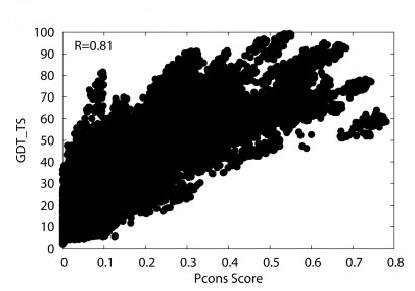
\includegraphics[scale=0.75]{pcons_correlation}
		\caption[Pcons vs GDT\_TS scattered plot]{Pcons vs GDT\_TS scattered plot.}
		\label{fig:pcons_corr}
	\end{center}
\end{figure}
Clustering methods tend to fail when the top models are far away from the cluster core or when no structural redundancy is present among the considered ensemble, determining a very sparse cluster. 
With the aim of avoiding these clustering drawbacks, QMEANclust \cite{Benkert2008ab, Benkert2008aa} uses QMEAN to select a subset of higher quality models. QMEANclust ranks models by computing the median of the distances between the current ranked model and all other models contained in the subset previously defined.\\
ModFOLDclust \cite{McGuffin2008} is a variant of the standard ModFOLD method. The global clustering score is based on the 3D-Jury \cite{Ginalski2003} method whereby each model is compared to every other model and the average structural similarity score is computed. ModFOLDclust differs from 3D-Jury, first in the use of the TMscore for pairwise comparisons and second in the server user interface allowing users to directly upload multiple models of their own choice from any source. A local MQAP version of ModFOLDclust also exists.


\cleardoublepage

	

\chapter{Materials and Methods}
\label{chap:materials_methods}

\section{Working Environment and Technologies}
\label{sec:working_environment_and_technologies}
The work performed in this thesis was developed at the Department of Biology\footnote{\href{http://dept.bio.unipd.it/}{http://dept.bio.unipd.it/}} of the University of Padua\footnote{\href{http://www.unipd.it/}{http://www.unipd.it/}}. The available hardware used to test the performance of the implemented method is a cluster of eight computers. Each of them is characterized by a bi-processor Intel Xeon 2.80GHz CPU with 2GB RAM. The objective of the installed cluster is to perform grid computing. Grids serve to manage the allocation of jobs to computers which will perform the work independently of the rest of the cluster. While each job is not affected by other jobs in progress on other nodes of the grid, in this installation, resources are shared by all nodes. In addition to these machines, a laptop computer is used as terminal to access remotely each cluster node. The latter is an AMD Turion64 X2, 1.60GHz CPU with RAM 2GB. Figure \ref{fig:cribi} illustrates the work architecture.\\
The method implemented during this thesis is experimental because, despite the clearly defined goal, the way to achieve a good solution depends highly on results. Due to this difficulty, a more agile approach with the aim to encourage frequent inspection and adaptation is used instead of standard project planning. Agile methodologies choose to do things in small increments with minimal planning, rather than long-term planning. Iterations are short time frames which typically last from one to four weeks. Each iteration is led by a team through a full software development cycle, including planning, requirements analysis, design, coding, unit testing, and acceptance testing when a working product is demonstrated to stakeholders. This helps to minimize the overall risk, and allows the project to adapt to changes more quickly. A SCRUM-based approach is adopted to manage and solve this problem. A high-level document for the entire project, called in the SCRUM terminology \emph{product backlog}, is defined at the beginning of the thesis and continuously monitored, in order to satisfy the main objectives and control eventual drifts. It contains a list of backlog items that are broad descriptions of all required features and wishlist items. The \emph{product backlog} answers to \emph{what} will be done. It also presents rough estimates of both business value and development effort that help to gauge the timeline and to manage priorities. Then, a more detailed short job document, called \emph{sprint backlog}, is written with the aim to describe detailed information about \emph{how} to implement the requirements for the upcoming sprint. In this thesis, each job is broken down into quarters (a quarter corresponds to two hours of work). For each job, estimated and measured times must be provided. Also, jobs can be made by human, e.g. programming or testing a software module, or by machine, e.g. computing an optimization. Finally, a priority is associated to each job with the aim to schedule an order among the activities. \\
The generation of different datasets and automatic execution over a set of targets is implemented in the Perl v5.8 programming language. Much of the source code requires the manipulation of strings and pattern matching functionalities. Moreover, an important non-functional requirement is also that a molecular biologist must be able to alter the source code in the near future. Perl is a high-level, interpreted scripting language that provides powerful facilities for text processing and manipulation of text files. It is a programming language also known by biologists, allowing to execute and manipulate variants of this current implementation in the future. Rather, all modules regarding the effective computation, such as neural networks and clustering, are implemented in C++ programming language for performance reasons. \\
From a software point of view, the Debian GNU/Linux distribution is used with the installed compiler GCC v4.1. The method realized during this thesis will become a package, called Osiris, of the \gls{VICTOR} library. It also depends on the \gls{FANN} v2.0 that offers lots of functions to deal with training and test sets of neural networks in an easy and versatile way, leaving to the user the configuration and validation tasks. In order to program all source code, the GNU Emacs v2.22.1 editor is chosen due to its usability and configurability. Statistics plots and tables shown in this thesis are generated using the GNU R package\footnote{Source: \href{http://www.r-project.org/}{http://www.r-project.org/}}, a free software environment for statistical computing and graphics, and the software Gretl v1.7.5\footnote{Source: \href{http://gretl.sourceforge.net/index.html}{http://gretl.sourceforge.net/index.html}}. UML diagrams are generated using Eclipse v3.4.2 IDE.
\begin{figure}[tb]
	\begin{center}
		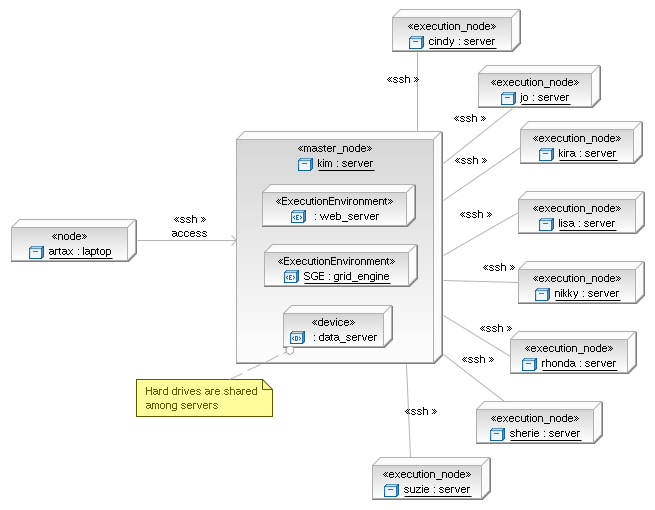
\includegraphics[scale=0.85]{cribi}
		\caption[Cluster of computers at CRIBI]{UML deployment diagram. All data resources are shared and located inside the Kim server. Every executive node is visible and accessible only by the Kim server which represents the master node. Registered users can run processes by SSH connection, all others by web interface if the web service is available.}
		\label{fig:cribi}
	\end{center}
\end{figure}



\section{How to Improve QMEAN}
\label{sec:howto_improve_qmean}
QMEAN \cite{Benkert2007, Benkert2008ab, Benkert2008aa, Tosatto2002} is a single-model scoring function based on a linear combination of a set of statistical potentials. A brief presentation dealing with statistical potentials is provided in Appendix \ref{sec:statistical_potentials}. The original idea of using such a scoring function composed by statistical potentials is found in \glslink{FRST}{FRST} \cite{Tosatto2005}. The last version of QMEAN scoring function, that is QMEAN6, can be described as follows:
\begin{equation}
	score = f(P_1, P_2, \ldots, P_6) = P_1w_1 + P_2w_2 + \ldots + P_6w_6
\end{equation}
where the vector \(\vec{P} = (P_1,P_2,\ldots,P_6)\) contains six features computed by QMEAN and the weight vector \(\vec{W} = (w_1,w_2,\ldots,w_6)\) is performed on the CASP-6 training set by using linear regression as implemented in the R package with the GDT\_TS score as target function.\\
The six features computed by QMEAN are the following:
\begin{description}
\item[Torsion 3-residue.] Extended torsion potential based on $\phi$ and $\psi$ propensities over three consecutive residues. Bin sizes: 45\textdegree\space for the center residue, 90\textdegree\space for the two adjacent residues.
\item[Solvation $C_\beta$.] Potential reflecting the propensity of a certain amino acid for a certain degree of solvent exposure based on the number of $C_\beta$ atoms within a sphere of 9 \AA{} around the center $C_\beta$.
\item[Pairwise $C_\beta$/SSE.] Residue specific pairwise distance dependent potential using $C_\beta$ atoms as interaction centers. Range 3-25 \AA{}, step size: 0.5 \AA{}. A secondary structure specific implementation was used both for the derivation and application of the potential.
\item[All-atom distance-dependent interaction.] Secondary structure specific interaction potential using all 167 atom types. The range is 3-20 \AA{} and the step size is 0.5 \AA{}.
\item[SSE PSIPRED.] Agreement between the predicted secondary structure of the target sequence using PSIPRED \cite{Jones1999aa} and the observed secondary structure of the model as calculated by the program \gls{DSSP} \cite{Kabsch1983aa}.
\item[ACCpro.] Agreement between the predicted relative solvent accessibility using SSPROACC \cite{Pollastri2007aa, Schuster1997aa} and the relative solvent accessibility derived from DSSP.
\end{description}
On the other hand, the weight vector is used to weight each parameter computed from the current protein model. The optimized weight vector is defined as:
\begin{equation}
\vec{W} = 
\left(
\begin{array}{c}
	w_{Torsion}\\
	w_{Solvation}\\
	w_{Pairwise}\\
	w_{All-atom}\\
	w_{SSE agreement}\\
	w_{ACC agreement}
\end{array}
\right) 
=
\left(
\begin{array}{c}
	-0.00185\\
	-0.00054\\
	-0.00062\\
	 -0.00108\\
	0.38072\\
	0.57997
\end{array}
\right)
\end{equation}

A scoring function of this type is immediate to implement and provides good solutions, even though it could be improved. Four possible ways to achieve this objective are described as follows:

\begin{description}
 \item[Non-Linear Method.] Different tertiary structure predictors are used to generate models for a given target sequence. Values computed from statistical potentials, which describe model properties, do not necessarily assume a linear behavior because they are depending on the model. For this reason, a non linear method should outperform the current linear weighed combination approach. In order to learn weights with the aim to deal with non-linear data, a \gls{SVM} or an \gls{ANN} could be used to.
 \item[Target Categorization.] QMEAN assumes input data quality to be uniformly distributed, while it is known that low quality models are much more fragment than median and high quality ones. A solution to this problem would be to consider different protein target classes separately. 
 \item[Using Density Information.] QMEAN is a single-model method, so it does not take into account density information. QMEANclust, the clustering version of QMEAN, was implemented because clustering-based methods perform better, as previously shown in \S~\ref{subsec:clustering_based_methods}. Therefore, it would be relevant and interesting to study a new strategy to include density information in the score computation.
 \item[Addition of New Features.] A good set of features describing the protein model forms the basis for a good single-model method. It is important that chosen features to be orthogonal among each other because the aim is to summarize well all main aspects of the predicted model. The research of new useful parameters could outperform the actual method.
 \end{description} 

\section{Description of the Osiris Package}
\label{sec:a_raw_neural_network}
The implemented system takes into account all previously cited improvements because:
\begin{itemize}
\item substitutes the QMEAN scoring function by using ANNs;
\item defines the quality of a model by considering its class also;
\item uses density information from an ensemble of models;
\item adopts other features in addition to those computed by QMEAN.
\end{itemize}
The study of ANNs has been inspired from information processing inside biological neural systems. In a neural network model, simple nodes, also called neurons or units, are connected together to form a network. ANNs are employed in statistics, cognitive psychology and artificial intelligence.\\
In this work, ANNs are trained following the supervised learning paradigm. In supervised learning, the network is trained by providing it with input and matching output patterns. These input-output pairs, also called training examples, are usually provided by hand or generated by a system component (self-learning). After this phase, network weights, inspired by neural synapses, are fixed and the system is ready to predict outputs from input samples. Most of the algorithms used in training artificial neural networks employ some form of gradient descent. A commonly used cost function is the \gls{MSE} which tries to minimize the average squared error between the network's output, $f(x)$, and the target value $y$ over all the example pairs. The most famous training algorithm based on gradient descent is backpropagation.\\
In order to capture density information on a data ensemble, clustering techniques are often used. Clustering is based on an unsupervised learning paradigm. In unsupervised learning, outputs are achieved by considering the relationships among a set of samples. Traditionally, clustering is referred to the assignment of objects into groups, called clusters, by computing a similarity or distance measure among objects.\\
More details on ANNs and clustering techniques are discussed in \cite{Baldi2001aa}, \cite{Mitchell1997aa}. The following subsections describe the system.

\subsection{Dataset Preprocessing}
\label{subsec:dataset_preprocessing}
The problem that MQAPs attemp to solve is quite particular. In fact, it requires the predictor to be quite general, but also able to distinguish little differences among models. To overcome these difficulties, a wide dataset is built in order to learn networks with a satisfactory number of samples.\\
In basic mode, features are represented by six parameters computed by QMEAN as shown in Figure \ref{fig:raw_ann}. They contain orthogonal information, meaning that each of them is independent enough from the others, and are not redundant. In all MQAPs, the output is a single real value in $[0, 1]$. Therefore, each ANN presents only an output unit, while the number of input units depends on how many features are considered. In order to build the dataset for the ANN, some previous activities are required. As shown in Figure \ref{fig:qmean_feature_generation}, it first needs to retrieve a target sequence $s$, a set of target models $M$ and the native structure $n$ related to the target sequence. QMEAN mainly requests three input parameters to execute:
\begin{description}
 \item [A target path:] a path containing a set of models $M$, in \gls{PDB} format, generated by tertiary structure predictors using the sequence $s$.
 \item [A file (*.horiz):] a file containing the secondary structure prediction of $s$, obtained by executing the program PSIPRED \cite{Jones1999aa}.
 \item [A file (*.sspro\_acc):] a file containing the secondary structure and solvent accessibility predictions of $s$, obtained by executing the program SSPROACC \cite{Pollastri2007aa, Schuster1997aa}.
\end{description}
The native structure and the TMscore program \cite{Zhang2004} are required in order to obtain the true model score, which serves in the learning phase.
\begin{figure}[tb]
	\begin{center}
		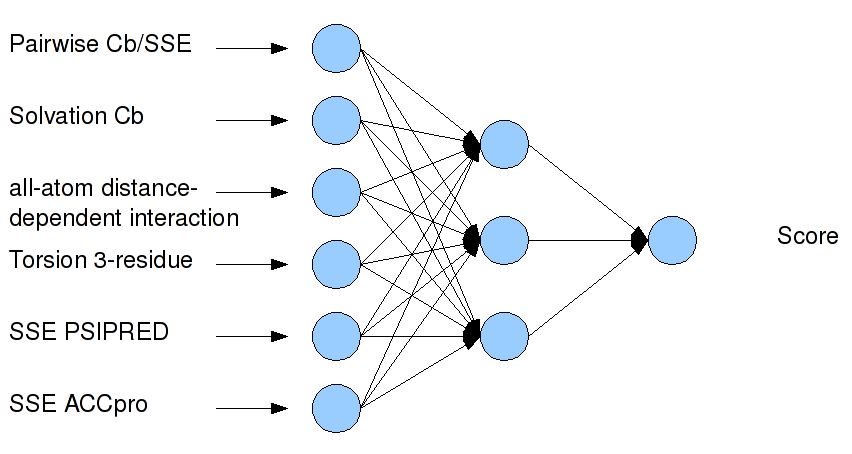
\includegraphics[scale=0.50]{raw_ann}
		\caption[Artificial neural network of six features from QMEAN]{Example of a simple ANN that receives as input six QMEAN features characterizing a model and returns a single output value that is the respective score.}
		\label{fig:raw_ann}
	\end{center}
\end{figure}
\begin{figure}[tb]
	\begin{center}
		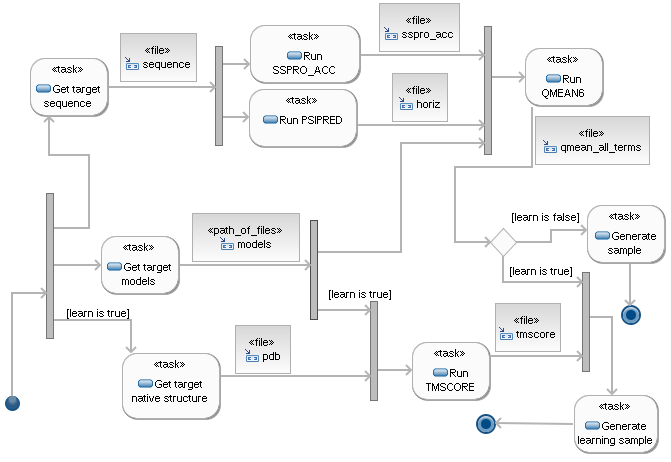
\includegraphics[scale=0.80]{qmean_feature_generation}
		\caption[Dataset generation UML diagram]{Conceptual activity UML diagram describing the key steps in order to obtain the dataset for the ANN. The procedure illustrated is summarised for one target and shows the data flow from the downloading step to the ANN dataset generation. Two areas could be distinguished: the QMEAN execution with the relative dependences and the TMscore execution. The first one is needed in order to obtain the six QMEAN features, while the second one is required when examples are used for learning the ANN, since it allows to associate the real model score. Therefore, in an operative phase of the ANN, the part of this diagram representing the TMscore execution is ignored. QMEAN features are scaled before being applied.}	
		\label{fig:qmean_feature_generation}
	\end{center}
\end{figure}

All target models used for training, that completely match another model of the same target are removed. In fact, it may happen that, for some different target models, QMEAN returns the same tuple of statistical potentials. For this reason, it is better to remove these redundant samples because they would deceive learning about the true data density distribution.\\
Since each QMEAN feature $f \in F$, where $F$ is the feature space, is defined in its own specific range, the values associated to that feature $f$ are previously scaled into the interval $[0, 1]$, before being used, in the following way:
\begin{enumerate}
 \item For each model $m \in M$, where $M$ is the set of all models of all target sequences, extract the previously computed value $v_f^{(m)}$ of the QMEAN feature $f$ and put it into vector $\vec{E}_f$.
 \item Store the minimum and the maximum value of the vector $\vec{E}_f$ in the variables $min_f$ and $max_f$ respectively.
 \item Compute the vector $\vec{N}_f$ by normalizing the vector $E_f$:
       \begin{equation}
       \label{eq:feature_normalization}
 	 \vec{N}_f(i) = \frac{\vec{E}_f(i) - min_f}{max_f - min_f}
       \end{equation}
       where $\vec{E}_f(i)$ is the $i$-th value of the vector $\vec{E}_f$, or in other words the value $v_f^{(m_i)}$ of the QMEAN feature $f$ computed for the $i$-th target model. 
\end{enumerate}
It is important to highlight that the minimum and maximum values of the feature $f$, respectively $min_f$ and $max_f$, are computed from data used for training, and stored in a file, with the aim to scale test data at a later time. Given a model used for testing the network, if the value associated to a feature $g$, overflows or underflows the admissible maximum or the minimum values for that feature, then that value will be approximated to $max_g$ in the overflow case or to $min_g$ otherwise.\\

\subsection{Training, Validating and Testing Phases}
\label{subsec:training_and_testing_phases}
During the learning phase, it is common to deal with two aspects: ANN selection and performance estimation. The former represents the choice of the \emph{optimal} parameters, e.g. learning parameters, network size and weights, for a certain classification or regression problem. The latter describes how to estimate the performance of the selected ANN.\\
The dataset is split into three subsets: 
\begin{itemize}
 \item Training set (TR): a set of examples used for learning over a certain tuple of classifier parameters.
 \item Validation set (VA): a set of examples used to tune the best tuple of classifier parameters.
 \item Test set (TE): a set of examples used only to assess the performance of a fully-trained classifier.
\end{itemize}
In order to train, validate and test the network, two different strategies can be considered: by target or by model. The first consists of considering each ANN sample as a target (which is composed of models), while the second one handles each sample as a model. The first strategy is chosen because allows a more effective distinction in samples used for training, validation or testing. In fact, it is possible that a subset of models generated for a certain target $t$ to be very similar. By considering ANN samples as protein models, the risk is to scatter two or more similar target models into two different subset, e.g. TR and VA, with the serious possibility of overestimating the network performance.\\
The training and validation sets are obtained by data from CASP-5, CASP-6 and CASP-7 (214 targets for a total of 78,854 models), while the test set is taken from CASP-4 (40 targets comprising 4,221 models) and CASP-8 (117 targets comprising 29,064 models). The test and validation sets are separated because it is known that the error rate estimate of the final model on validation data will be biased (lower than the true error rate) since the validation set is used to select the final ANN. The main procedure used to train, validate and test the network implemented is the following:
\begin{enumerate}
 \item Divide all the data into three partitions: training, validation and test set.
 \item Select the architecture and training parameters.
 \item Train the ANN using the training set.
 \item Evaluate the ANN using the validation set.
 \item Repeat step 2 through 4 using different architectures and training parameters.
 \item Select the best ANN and train it using data from the training and validation set.
 \item Assess this final ANN using the test set.
\end{enumerate}
Since K-fold cross validation is applied, steps 3 and 4 are repeated for each of the K folds. Then, the best ANN, see the $6^{th}$ step above, is the network having the minimum MSE (the minimum over a set of averaged MSEs obtained in step 4). The following subsections describe in detail the components of the procedure described above.

\subsubsection{Training}
\label{subsubsec:training}
All adopted ANNs are feed-forward. In feed-forward neural networks, the information moves in only one direction (forward) from the input, through the hidden to the output nodes without recurring cycles. The training algorithm used is Resilient backpropagation, Rprop, a local adaptive learning algorithm. Rprop is choosen with respect to other training algorithms such as Batch, Incremental or Quickprop for a series of reasons. First, it reduces the number of freely adjustable parameters, e.g. the learning rate, a problem that leads to a tedious search in the parameter space. Second, it is commonly considered a fast general purpose training algorithm. Third, it gives the best performance in the current described method. More details about the Rprop algorithm can be found in \cite{Riedmiller1994, Riedmiller1992}. Initial weights are small random values comprised in the real range $[-0.1, 0.1]$ in order to improve the gradient descent from a numerical point of view. The training stop function used is the MSE, set to suspend training when the desired error is 0 unless the maximum or stagnation number of epochs are reached. 
Two training modes are investigated: 
\begin{itemize}
 \item Fixed topology training. The training phase aims to find the \emph{optimal} weights by using a backpropagation-based training algorithm. All fixed topology ANNs trained in this work are composed by only one hidden layer, obtaining in this way networks of three layers. The activation function for the input, hidden and output units is the sigmoid whose output range is $[0, 1]$, defined as:
 \begin{equation}
  	f(x) = \frac{1}{1 + e^{-2sx}}
 \end{equation}
where $s$ is the steepness, set to $0.5$.
 \item Variable topology training. In order to know, understand and experiment different learning methods, a new type of algorithm is also taken into account: Cascade-Correlation. This algorithm begins with a minimal neural network and then automatically trains and adds new hidden units, also called candidate units, one by one, creating a multi-layer structure. For each new hidden unit that has been added to the network, its input-side weights are frozen (see Figure \ref{fig:cascade_net}). The Cascade-Correlation algorithm allows very quick learning, without requiring backpropagation. Moreover, there is no need to guess the size, depth and connectivity of the network in advance simplifying user configuration. A more complete elucidation dealing with the Cascade-Correlation learning architecture is reported in \cite{Fahlman1990}. In this work, all trained Cascade-Correlation architectures are fully connected networks with shortcut connections. Shortcut connections are connections that skip layers.  A fully connected network with shortcut connections is a network where all neurons are connected to all neurons in later forward layers, including direct connections from the input layer to the output layer. The maximum number of epochs is mantained to $150$ as default for both hidden and output units, and the stagnation number of epochs is kept to $12$. The number of cascade candidate stagnation epochs represents the number of epochs in which training is allowed to continue without changing the MSE by a fraction of $0.01$. Because every candidate unit is trained individually, there is no need to set up the same activation function. In other words, the algorithm chooses the most fitting activation function among sigmoid, symmetric sigmoid (hyperbolic tangent), gaussian and symmetric gaussian, using the following default activation steepnesses $0.25$, $0.5$, $0.75$, $1$ respectively. The activation function for the output unit is sigmoid configured with steepness of $0.5$.
\end{itemize}
\begin{figure}[tb]
	\begin{center}
		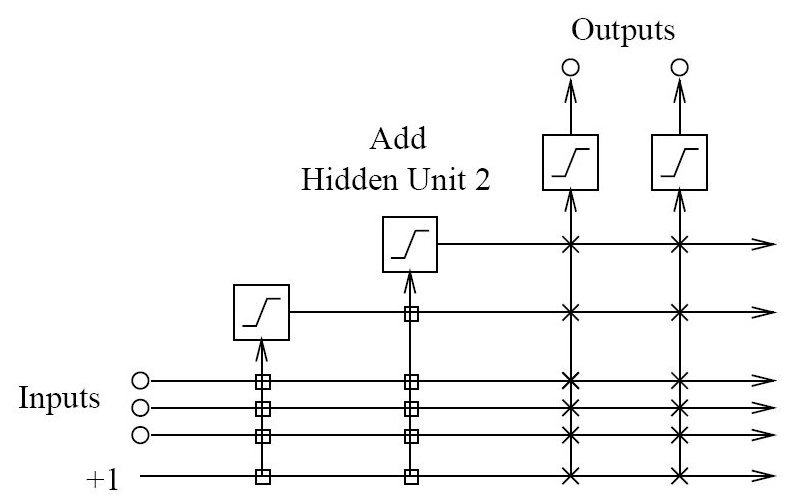
\includegraphics[scale=0.50]{cascade_net}
		\caption[The Cascade-Correlation architecture]{The Cascade-Correlation architecture after adding two hidden units. Each new hidden unit receives a connection from both every original input units and pre-existing hidden units. Its input weights are frozen at the time the unit is added to the net. This fact is represented with boxed connections ($\Box$). Instead, output connections, described as cross connections ($\times$) are trained repeatedly.}
		\label{fig:cascade_net}
	\end{center}
\end{figure}


\subsubsection{Validation}
\label{subsubsec:validation}
The choice for the best parameters to configure a neural network is a fundamental and difficult aspect that determines the quality of the predictor. Only the most important parameters are investigated in order to fit the best values. For fixed topology ANNs, the number of epochs and hidden units are taken into account, in the range $[1, 5000]$ with step $250$ and $[2, 5]$ with step $1$ respectively.
For variable topology ANNs, only the number of hidden units is considered in the range $[1, 25]$ with step $1$.\\
With the intent of having a better accuracy for the generated ANN, K-fold cross validation is used. This technique consists in creating a K-fold partition of the dataset (TR + VA). For each of the K experiments, $K-1$ folds are used for training and the remaining one for validating the obtained ANN, as shown in Figure \ref{fig:kfoldcrossvalidation}. The advantage of K-fold cross validation over other techniques, e.g. Random Subsampling, is that all dataset samples are eventually used for both training and testing. The true error is estimated as the average error rate:
 \begin{equation}
  	\tilde{E} = \frac{1}{K}\sum_{i=1}^{K}E_i
 \end{equation}
where $E_i$ is the MSE when the validation set is the $i$-th fold. 

\begin{figure}[tb]
	\begin{center}
		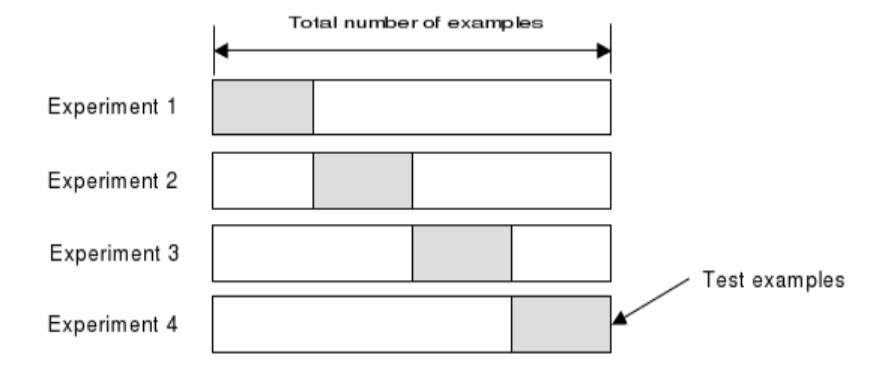
\includegraphics[scale=0.65]{kfoldcrossvalidation}
		\caption[K-fold cross validation]{Example of K-fold cross validation.}
		\label{fig:kfoldcrossvalidation}
	\end{center}
\end{figure}
In order to achieve small values for the \glslink{bias}{bias} and \glslink{variance}{variance} of the true error rate estimator and to reduce computation time, the parameter K is set to $5$. In fact, with a large number of folds, the bias will be small (that means that the estimator will be very accurate), but the variance and computation time (that depend on the number of experiments) will be very large. On the other hand, with a small number of folds, the variance and computation time are reduced, but the bias of the estimator will be large. Moreover, since the original training set, composed by both TR and VA is very large, $5$-fold cross validation yields a good accuracy. A review about the most important accuracy estimation methods can be found in \cite{Kohavi1995}.
% folds obtained by using (mod 4). no data randomization before splitting into folds. skip

\subsubsection{Testing}
\label{subsubsec:testing}
The implemented individual methods are very fast. In fact, after having trained the neural network, the execution involves only the information processing from input to output units. Although the training process requires several hours to complete, due to the training set width, the running process only depends on the number of neural units that are used and this number is constant. In order to test the network performance, two different datasets are used, one from CASP-4 and the other from CASP-8. The first is made of relatively simple targets, while the second, proposed in 2008, comprises a wide target set of different difficulty for quality assessment. Performance evaluation is usually based on a measure of global correlation. This measure also allows to compare the implemented method with other related work. Here, correlation indicates a linear relationship between two random variables that represent the true and predicted score, giving a value in the range $[-1,+1]$. If the correlation is $1$, then the two random variables are identical. The correlation reflects only the noisiness and direction, but not the slope of that relationship.
At CASP, the measure to assess a model score is GDT\_TS. The true score of a model can be obtained by using the program TMscore measuring the similarity between the given protein model and the relative native structure. The predicted score of a model is determined by the MQAP. Here, the focus is on the global correlation of a method, which stands for the correlation whose data are all models of all given targets. The Pearson and Spearman correlations are used together in order to understand more accurately the results. Moreover, for the CASP-8 test set, a comparison with the best MQAPs is provided.



\subsection{Target Categorization}
\label{subsec:target_categorization}
The idea is to handle targets differently with respect to their category in order to increase the accuracy in general. Hence, a formulation of categorization and a manner to use the classification information are required. The key point is that models are generated by different types of tertiary structure predictors and this information determines the obtained model quality. Figure \ref{fig:model_distribution_in_casp567} reports the quality distribution of models coming from CASP-5, CASP-6 and CASP-7.
\begin{figure}[tb]
	\begin{center}
		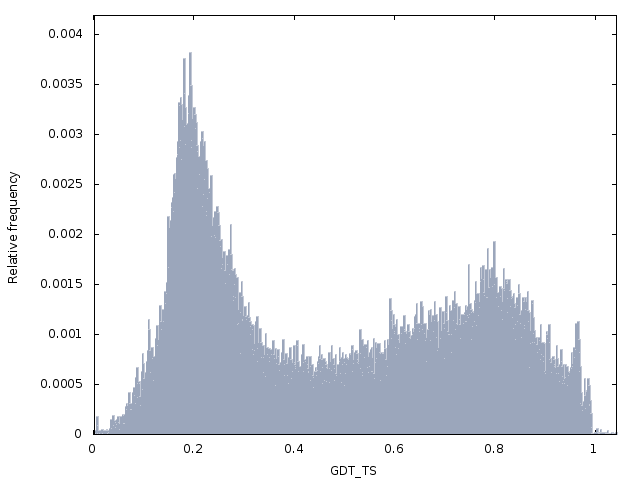
\includegraphics[scale=0.60]{model_distribution_in_casp567}
		\caption[Mixture of Gaussian distributions describing the model frequency with respect to the quality]{Mixture of Gaussian distributions describing the model frequency with respect to the quality. Distributions are obtained by using 78,854 models from CASP-5, CASP-6 and CASP-7.}		
		\label{fig:model_distribution_in_casp567}
	\end{center}
\end{figure}
Two main Gaussian distribution are separated approximately at the threshold $\theta = 0.41$ GDT\_TS. The first distribution contains raw or wrong models typically obtained by using \emph{ab initio} or \emph{novel fold} methods. These models are called \glslink{FM}{Free Models (FM)}. The second one instead contains more accurate models mostly obtained by using comparative modelling or fold recognition techniques. These models are called \glslink{TBM}{Template-Based Models (TBM)}. A more detailed distinction could further be achieved in the TBM distribution. In fact, it could be split again into medium and high quality classes, as shown in Figure approximately at the threshold $\psi = 0.77$ GDT\_TS. By this distinction, models with score in the range $(\theta,\psi]$ are called TBM, whereas models with score greater than $\psi$ are called \glslink{HQM}{High Quality Models (HQM)}. This last distribution contains models that are very similar to the native structure. Therefore, an accurate quality assessment for HQM models is much more important than that for TBM or FM models. The goal is to apply this classification also to the implemented method, in order to refine the prediction method (see Figure \ref{fig:system_execution}), while considering target instead of model classification. The idea is to decompose a problem so that it is dealt with by three modular expert components (FM\_ANN, TBM\_ANN and HQM\_ANN), each of which is designed as a specific function approximator \cite{Sharkey96aa,MuiAGW94aa,FrosyniotisSL03aa,Happel1994aa,Schmidt1996aa}. In this way, every component of the neural network system can be different from the others by varying the architecture, feature space (see \S~\ref{subsec:addition_of_new_features}) and dataset. By adopting a modular architecture, each module could be trained in parallel, improving the computation time. Also, by splitting the dataset into classes and training a module using only data from a class, the non-linear function to learn is obviously simpler, because more specific, and thus the training is faster. 
Algorithm \ref{algo:target_classification} describes the target classification.
\begin{algorithm}
\caption{$ClassifyTarget(Target)$}
\label{algo:target_classification}
\begin{algorithmic}[1]
\REQUIRE $Target \neq \emptyset$
\ENSURE $Target$ is classified
\STATE $\theta \leftarrow 0.41$
\STATE $\psi \leftarrow 0.77$
\STATE $\tilde{t} \leftarrow MedianScore(Target))$
\STATE $Class(Target) \leftarrow null$
\IF{$\tilde{t} \leq \theta$}
	\STATE $Class(Target) \leftarrow FM$
\ELSIF{$\tilde{t} \leq \psi$}
	\STATE $Class(Target) \leftarrow TBM$
\ELSE [$\tilde{t} > \psi$]
	\STATE $Class(Target) \leftarrow HQM$
\ENDIF
\RETURN $Class(Target)$
\end{algorithmic}
\end{algorithm}
The median is preferred in this case over the mean because it is more robust regarding outliers. An outlier is an observation that is numerically distant from the rest of the data, generating skewed distributions. For each target sequence, models typically form a skewed distribution since FM predictors build many more models than TBM or HQM predictors. The median better balances this fact.\\
Target classification is proposed instead of model classification as it allows to associate a class by considering a set of models. Methods learn better by using target classification since classes are not completely disjoint, but contain overlapping information that is characterized by models (outliers) that would belong to a different class with respect to their target one.
\begin{figure}[tb]
	\begin{center}
		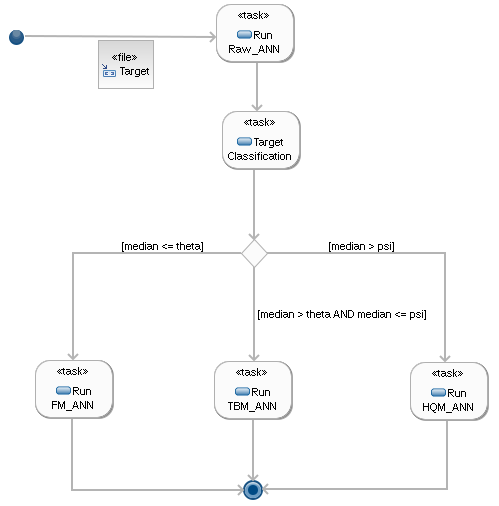
\includegraphics[scale=0.85]{system_execution}
		\caption[Control flow of the neural system]{UML activity diagram showing the control flow of the neural system. A raw ANN is trained without considering differences in the distribution of models. Three expert ANNs are trained only on specific classes: FM, TBM and HQM. ANNs compute a GDT\_TS score in the range $[0, 1]$. For each target, the median of model scores that have been predicted by the Raw\_ANN is calculated. In this way, the Raw\_ANN is used both to predict a score for each model and to classify targets. After being categorized, a target is sent to the expert ANN associated to its class. There is no score combination at the end of the process, as common in modular approaches, but only a data splitting after applying the Raw\_ANN.}
		\label{fig:system_execution}
	\end{center}
\end{figure}


\subsection{Density Information}
\label{subsec:density_information}
Clustering methods are recognized to be very accurate in model quality assessment. In this kind of programs, a set of models is evaluated by considering similarities among models. The idea is to use the density information after having applied a MQAP method, e.g. QMEAN or ANN with features from QMEAN. In order to measure similarities between two models, the GDT\_TS quality measure is adopted. Given two models $m$ and $n$, the GDT\_TS similarity has, by definition, the following properties:
\begin{enumerate}
 \item $GDT\_TS(m, n) \geq 0$ and $GDT\_TS(m, n) \leq 1$.
 \item $GDT\_TS(m, n) = 1$ if and only if $m = n$.
 \item $GDT\_TS(m, n) = GDT\_TS(n, m)$.
\end{enumerate}
It is important to highlight that the GDT\_TS measure is not a distance since it does not satisfy the triangle inequality. This fact is shown by using a counterexample. Given three models $r$, $s$ and $t$ where $r$ and $s$ are very similar, e.g. $x = GDT\_TS(r, s) = 0.9$, while $t$ is very different from the previous two models, e.g. $y = GDT\_TS(r, t) = 0.1$ and $z = GDT\_TS(s, t) = 0.2$, in order to satisfy the triangle inequality, the following conditions must be valid $x \leq y + z$, $y \leq x + z$ and $z \leq x + y$. However the first condition is false because $0.9 \nleq 0.1 + 0.2$.\\
A similarity matrix is computed for any target $T$ by computing the GDT\_TS between each pair of target models. This matrix is squared, symmetric and has diagonal $1$ due to the above properties. Thus, only the upper or lower triangle with respect to the diagonal needs to be computed. In other words the matrix describes the similarities of each model with respect to the others. Therefore, the clustering process serves to calculate a score that takes into account the similarities between the current model and the other models. \\
Instead of considering all models to assess the score of a given model, a better solution is to use only a subset of the best models, building up a semi-clustering procedure. The idea is to limit the well-known clustering drawback, that is the loss of the best models which are far from the center of the main cluster. Very bad models represent outliers in the whole target distribution and, for this reason, should be eliminated from the clustering computation. The semi-clustering approach is illustrated in Figure \ref{fig:semi_clustering}.\\
\begin{figure}[tb]
	\begin{center}
		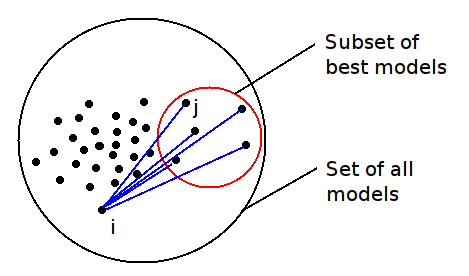
\includegraphics[scale=0.8]{semi_clustering}
		\caption[The semi-clustering approach]{The semi-clustering approach. A previous MQAP (e.g QMEAN) provides an estimation of the quality of each target model. An optimized percentage value, computed over target models of CASP-5, CASP-6 and CASP-7 and specific for FM, TBM and HQM targets, defines the size of the best subset. In this semi-clustering approach, only the subset of the best models is dealt with, instead of considering all target models. The lines between model $i$ and models in the best subset represent the similarities (not the distances). In order to score model $i$, the mean of these similarities, weighted by the previous MQAP scores of the best models used, is calculated. Finally, the computed mean is weighted by the $PFractionModelled$ of the model $i$.}
		\label{fig:semi_clustering}
	\end{center}
\end{figure}
A way to obtain such a subset is to consider a percentage of the best scores achieved by an other MQAP, i.e. QMEAN, used as support method. A specific percentage is optimized over target models from CASP-5, CASP-6 and CASP-7 datasets for the FM, TBM and HQM targets, using QMEAN as support MQAP (see \S~\ref{subsec:semiclustering_optimization}). The best percentages are obtained in the following way. First of all, targets are split into the three categories FM, TBM and HQM. Therefore, for each class, by varying the percentage of the best models, each target is clustered and a class Pearson correlation is computed between the cluster scores and the real scores. Finally, the best percentage of each class, that is the value corrisponding to the highest Pearson correlation for the class, is found. The optimization plots for FM, TBM and HQM models respectively are proposed in \S~\ref{subsec:semiclustering_optimization}. Algorithm \ref{algo:optimize_percentages} describes the optimization.\\
% NOTE: NO \COMMENT{} directly after \FOR |WHILE |FORALL loops
\begin{algorithm}
\caption{$OptimizePercentages(Targets)$}
\label{algo:optimize_percentages}
\begin{algorithmic}[1]
\REQUIRE $Targets \neq \emptyset$
\ENSURE A percentage for each class (FM, TBM, HQM)
\STATE $FMset \leftarrow \{T \in Targets$ such that $Class(T) = FM\}$
\STATE $TBMset \leftarrow \{T \in Targets$ such that $Class(T) = TBM\}$
\STATE $HQMset \leftarrow \{T \in Targets$ such that $Class(T) = HQM\}$
\STATE $Classes \leftarrow \{FMset, TBMset, HQMset\}$
\FOR{each class $C$ such that $C \in Classes$}
	\STATE $RealScores \leftarrow \emptyset$
	\FOR{each target $T$ such that $T \in C$}
		\STATE $Add(RealScores, RealScore(T))$
	\ENDFOR	
	\FOR{$\lambda=0.05$ step $0.01$ to $1.0$}
		\STATE $PERCENTAGE_C \leftarrow \lambda$
		\STATE $ClusterScores \leftarrow \emptyset$
		\FOR{each target $T$ such that $T \in C$}
			\STATE $Add(ClusterScores, Clustering(T))$
		\ENDFOR
		\STATE $Pearson \leftarrow PearsonCorrelation(RealScores, ClusterScores))$
		\PRINT $(\lambda, Pearson)$
	\ENDFOR
\ENDFOR
\end{algorithmic}
\end{algorithm}
Sometimes a predicted model is incomplete, in the sense that only a part of the target sequence is modelled. The $FractionModelled$ feature, computed by QMEAN, represents the percentage of modelled structure. By applying the $FractionModelled$ descriptor, the effect gained is to reduce the final scores of incomplete models. In other terms, it lowers the presence of false positive models, e.g. structures where the modelled part is well predicted, causing the MQAP to assign a high score to those models, regardless of being incomplete. By weighting models for their fraction modelled, more correct scores are achieved. However, the pure $FractionModelled$ application sometimes penalizes too much the model scores. In order to overcome this drawback, a solution may be to use another feature computed from the known $FractionModelled$. The aim is that this new feature does not penalize too much nearly complete models but is able to lower the score of false positive models previously discussed. A function that satisfies these requirements is the following:
 \begin{equation}
  	f(x) = -x^2 + 2x
 \end{equation}
where $x \in [0, 1]$ is the common $FractionModelled$ feature. This new function, called $PFractionModelled$, where $P$ stands for Parabolic, performs better than the usual one as shown in \S~\ref{subsec:parabolic_fraction_modelled}. Figure \ref{fig:parabolic_fraction_modelled} shows the function $PFractionModelled$. 
\begin{figure}[tb]
	\begin{center}
		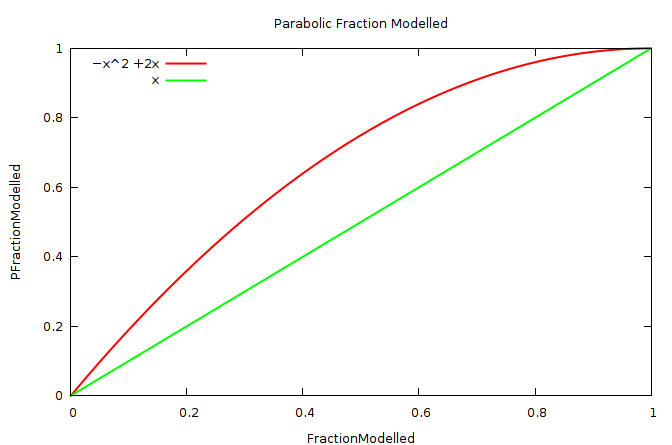
\includegraphics[scale=0.6]{parabolic_fraction_modelled}
		\caption[Parabolic Fraction Modelled function]{Parabolic Fraction Modelled function. By using this function, cluster scores are less affected by the computed fraction modelled of the structure.}
		\label{fig:parabolic_fraction_modelled}
	\end{center}
\end{figure}
It is important to highlight that the $FractionModelled$ feature is purely quantitative because it does not take into account that protein regions may have different importance. For example, given two identical protein models, their $FractionModelled$ could be the same also if the first one misses a piece of polypeptide backbone concerning the active site whereas the second a piece less important. However, the second model quality is clearly greater than the first one. Computing a $FractionModelled$ in order to consider differently the modelled parts is a hard task because it needs to recognize which parts are more important than others. The $PFractionModelled$ feature implicitly assumes that small faults in the model constitute almost trascurable errors, whereas larger faults represent important mistakes. This assumption is consistent with the observed data (see \S~\ref{sec:protein_structure_prediction}).\\
Algorithms \ref{algo:get_discrimination_score} and \ref{algo:target_clustering} describe the clustering subroutines.
\begin{algorithm}
\caption{$DiscriminatingScore(Target)$}
\label{algo:get_discrimination_score} 
\begin{algorithmic}[1]
\REQUIRE $Target \neq \emptyset$
\ENSURE The score of the worst model $m \in BestModels(Target)$. This score discriminates the best models from all others.
\STATE $\tau \leftarrow PERCENTAGE_{Class(Target)}$
\COMMENT{$PERCENTAGE_{Class(Target)} \in (0,1]$ is the optimized percentage referred to the $Target$ class. Classes are FM, TBM and HQM.}
\STATE $SortedScore \leftarrow Score(Target)$
\STATE $n \leftarrow Size(SortedScore)$
\FOR{each model $m$ such that $m \in Target$}
	\STATE $SortedScore[m] \leftarrow SortedScore[m] * PFractionModelled(Target, m)$
\ENDFOR
\STATE $SortedScore \leftarrow Sort(SortedScore)$
\STATE $DiscrimPos \leftarrow n - (n * \tau)$
\COMMENT{If $\tau \rightarrow 0^{+}$ then $DiscrimPos \rightarrow n^{-}$. Due to approximations this could lead to a buffer overflow of one element. By assumption, the element in position $(DiscrimPos-1)$ always exists and corresponds to the last (the greatest) element of $SortedScores$.}
\IF{$DiscrimPos = n$}
	\RETURN $SortedScore[DiscrimPos - 1]$
\ENDIF
\RETURN $SortedScore[DiscrimPos]$
\end{algorithmic}
\end{algorithm}
\begin{algorithm}
\caption{$Clustering(Target)$}
\label{algo:target_clustering}
\begin{algorithmic}[1]
\REQUIRE $Target \neq \emptyset$
\ENSURE A new score for each model $m \in Target$
\STATE $Sum \leftarrow 0$
\STATE $WeightedSum \leftarrow 0$
\STATE $TempScore \leftarrow 0$
\STATE $Threshold \leftarrow DiscriminatingScore(Target)$
\STATE $ClusterScore(Target) \leftarrow \emptyset$
\FOR{each model $m$ such that $m \in Target$}
	\STATE $Sum \leftarrow 0$
	\STATE $WeightedSum \leftarrow 0$
	\FOR{each model $n$ such that $n \in Target$}
		\IF{$Similarity(Target, m, n) \neq 0$ and\\ 
		    $(Score(Target, n) * PFractionModelled(Target, n)) \geq Threshold$}
			\STATE $Sum \leftarrow Sum + Score(Target, n)$
			\STATE $WeightedSum \leftarrow WeightedSum + $\\
			       $(Similarity(Target, m, n) * Score(Target, n))$
			\COMMENT{$Score(Target, n)$ is not weighted by $PFractionModelled(Target, n)$.}
		\ENDIF
	\ENDFOR
	\STATE $TempScore \leftarrow (WeightedSum / Sum) * PFractionModelled(Target, m)$
	\STATE $Add(ClusterScores(Target), TempScore)$
\ENDFOR
\RETURN $ClusterScores(Target)$
\end{algorithmic}
\end{algorithm}
The algorithm used to cluster target models has a running time of $0(n^{2})$ where $n$ is the number of models proposed for a certain target. In practice, $n$ has values between $200$ and $400$. To improve the method performance, the similarity matrices can be computed once previously to the clustering process.



\subsection{Addition of New Features}
\label{subsec:addition_of_new_features}
The last approach adopted to improve QMEAN includes the addition of new features. Feature selection is an important, but also hard, task that has the aim to find a set of effective, non redundant and independent protein descriptors. The intent is to define new ANNs based on features retrieved from both QMEAN and other methods.\\
Three new features are taken into account: Gauss integrals, hydrogen bonds and TAP score. The following subsections describe these features and how they are combined together with QMEAN. All additional features, with ranges in the interval $[0, 1]$, are scaled by using the equation \ref{eq:feature_normalization}.

\subsubsection{Gauss Integrals}
\label{subsubsec:gauss_integrals}
An interesting and new way to describe proteins from a geometrical point of view is represented by Gauss integrals \cite{Rogen2005,Rogen2003,Rogen2003b}. They are protein shape descriptors, independent of translation and rotation, that are able to distinguish among similar, but still different morphologies. Generalized Gauss integrals arise from Vasiliev knot invariants and deal with crossings seen in all planar projections of curves representing the protein polypeptide chain. Crossings have a sign defined by the right-hand rule (see Figure \ref{fig:link_crossings}). The generalized Gauss integrals used in this work are based on the writhe and average crossing number of first, second and third orders. The writhe is the total number of positive crossings minus the total number of negative crossings, whilst the average crossing number of a curve is the unsigned average number of crossings seen in the different planar projections of the curve (see Figure \ref{fig:labeled_whitehead_link}).
\begin{figure}[tb]
	\begin{center}
		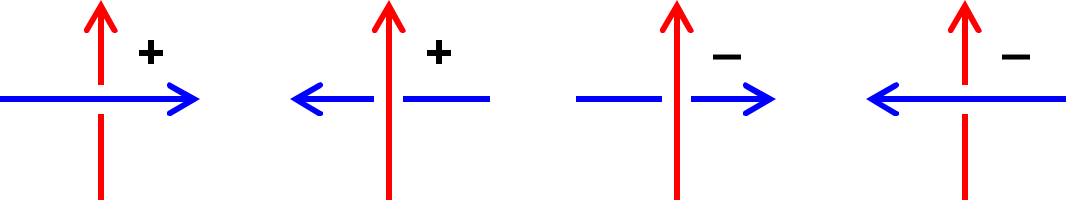
\includegraphics[scale=0.35]{link_crossings}
		\caption[Positive and negative crossings]{Examples of positive and negative crossings.}
		\label{fig:link_crossings}
	\end{center}
\end{figure}
\begin{figure}[tb]
	\begin{center}
		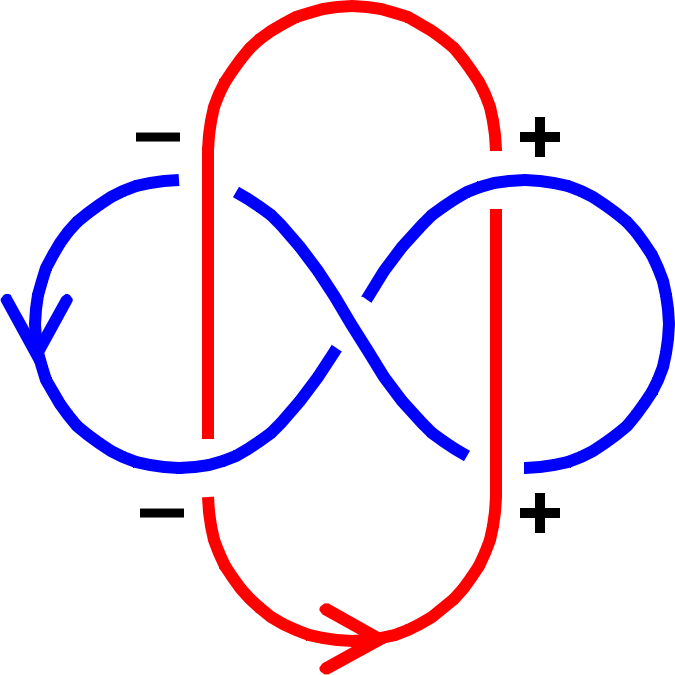
\includegraphics[scale=0.30]{labeled_whitehead_link}
		\caption[Example of crossings seen in two curves]{Example of crossings seen in two curves.}
		\label{fig:labeled_whitehead_link}
	\end{center}
\end{figure}
A more detailed explanation and formalization of Gauss integrals is reported in Appendix \ref{appendix:gauss_integrals}.
The program used to compute Gauss integrals is called \gls{GIT}. GIT can operate in two modes. The first calculates Gauss integrals by considering exactly protein backbone $C_\alpha$ atoms, whereas the second deals with a \emph{smoothed} version of the protein backbone. The first mode is chosen by exclusion, because the second one is not stable in the generation of Gauss integrals. The low reliability of the results for the second mode might be associated to the fact that protein models and not experimental structures are considered in this work. 
Instead of using all computed $29$ descriptors, the most informative ones, i.e. the more discriminative among all $29$ Gauss integrals, are taken into account by considering Ba\'{u}'s work \cite{Bau2008}. The following $7$ Gauss invariants were selected: $I_{(1,2)}$, $I_{(1,2)(3,4)}$, $I_{(1,2)(3,4)(5,6)}$, $I_{(1,2)(3,5)(4,6)}$, $I_{(1,2)(3,6)(4,5)}$, $I_{(1,4)(2,3)(5,6)}$ and $I_{(1,6)(2,3)(4,5)}$. 



\subsubsection{Hydrogen Bonds}
\label{subsubsec:hydrogen_bonds}
A hydrogen bond is the attractive force between an electronegative atom and a hydrogen covalently bound to another electronegative atom. It results from a dipole-dipole force with a hydrogen atom bound to fluorine, nitrogen or oxygen (see Figure \ref{fig:os_wat2}).
These bonds can occur between molecules (intermolecularly), or within different parts of a single molecule (intramolecularly). A hydrogen bond is a very strong fixed dipole-dipole van der Waals force, but weaker than covalent, ionic bonds. It is somewhere between a covalent bond and an electrostatic intermolecular attraction. This type of bond occurs in both inorganic molecules (such as water) and organic molecules (such as DNA) (see Figure \ref{fig:quadruple_hydrogen_bond}). 
The length of hydrogen bonds depends on bond strength, temperature, and pressure. The bond strength itself is dependent on temperature, pressure, bond angle, and environment. The typical length of a hydrogen bond in water is 1.97 \AA.\\
Hydrogen bonds plays an important role in determining the three-\-di\-men\-sio\-nal protein structures. In such macromolecules, bonds between parts of the same macromolecule are partially responsible to the folding process. Hydrogen bonds form between the backbone oxygens and amide hydrogens and contribute to the formation of alpha helices and beta sheets. Hydrogen bonds also play a part in forming the tertiary structure of proteins through interaction of $R$-groups. For these reasons, the use of hydrogen bond-based features should be relevant. In order to compute hydrogen bonds, the program HBPLUS \cite{McDonald1994aa} is adopted. The application returns the number of hydrogen bonds found in a three-\-di\-men\-sio\-nal protein and this number is used as feature.
\begin{figure}[tb]
	\begin{center}
		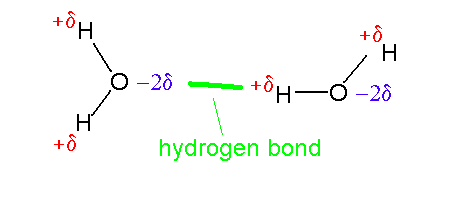
\includegraphics[scale=0.70]{os_wat2}
		\caption[Example of hydrogen bond between two water molecules]{Example of hydrogen bond between two water molecules.}
		\label{fig:os_wat2}
	\end{center}
\end{figure}

\begin{figure}[tb]
	\begin{center}
		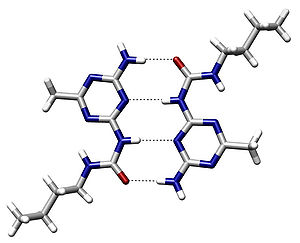
\includegraphics[scale=0.80]{quadruple_hydrogen_bond}
		\caption[Example of intermolecular hydrogen bonding]{Example of intermolecular hydrogen bonding in a self-assembled dimer complex (See \cite{Beijer1998sca}).}
		\label{fig:quadruple_hydrogen_bond}
	\end{center}
\end{figure}

\subsubsection{TAP score}
\label{subsubsec:tap_score}
TAP score \cite{Tosatto2007aa} is a recent criterion for measuring, in a quantitative way, the sequence to structure compatibility based on the normalization of torsion angle propensities including the side chain. The normalization involves the definition of the global minimum and maximum of the protein sequence. TAP score is used to recognize the best experimental structures.\\
TAP score estimates the quality of a protein model based on the Ramachandran plot of the backbone ($\phi$, $\psi$) torsion angles, thus it is based on conformational criteria. While each amino acid type may, in theory, adopt a large number of different conformations, here, large areas of the Ramachandran plot are almost empty. This is due to steric clashes deriving from the local geometry of the polypeptide chain. TAP score simultaneously combines five different torsion angles into a single pseudo-energy value. Adding more torsion angles is known to improve the overall discrimination of protein decoys, as it captures the subtle interplay between them. TAP score explores the avenue of capturing the interplay between protein backbone and side chain. \\
One benefit of adopting a modular approach to ANNs is the possibility to employ a set of specific features for a certain module of the neural system \cite{Happel1994aa}. Since TAP score is indicative to assess scores for high quality structures, the idea is to use it as a feature for only high quality targets that are predicted by the HQM expert ANNs.

%    - the final system (QMEAN + raw_ann + expert_anns + cluster)


\cleardoublepage

	

\chapter{Results and Discussion}
\label{results}
This thesis basically defines $5$ new methods: $2$ single model-based and $3$ clustering-based. For each of them, features from QMEAN are considered as input. It is important to highlight that the new implemented clustering algorithm does not depend on a QMEAN-based method, but could use a generic MQAP as support to weight model scores. Trying other MQAPs as support methods may be an interesting test to do in the near future with the intent to further outperform the reported results.
The main descriptions of the methods proposed are the following:
\begin{description}
	\item[QMEANrannZ:] The final model score is achieved by a single raw neural network.
	\item[QMEANeannZ:] The target model scores of QMEANrannZ are used to classify the relative target in the FM, TBM or HQM classes. Then, the target models are scored by an expert neural network, associated to that category.
	\item[QMEANrannclustZ:] The implemented clustering algorithm uses QMEANrannZ as support MQAP.
	\item[QMEANeannclustZ:] The implemented clustering algorithm uses QMEAN\-eannZ as support MQAP.
	\item[QMEANclustZ:] The implemented clustering algorithm uses QMEAN as support MQAP.
\end{description}

The reported results distinguish whether the used ANNs have a fixed or a ca\-sca\-de-\-cor\-re\-la\-tion architecture.\\
In addition to the above methods, experiments also involve new features aside from those standard for QMEAN, such as Gauss integrals, hydrogen bonds and TAP score (see \S~\ref{subsec:addition_of_new_features}). Therefore, depending on the features utilized, the following different schemes are proposed:
\begin{description}
\item[std\_median] All ANNs use only features from QMEAN (neural networks with $6$ input units).
\item[std\_G\_median] All ANNs use features from QMEAN and GIT (neural networks with $13$ input units).
\item[std\_H\_median] All ANNs use features from QMEAN and HBPLUS (neural networks with $7$ input units).
\item[std\_GH\_median] All ANNs use features from QMEAN, GIT and HBPLUS (neural networks with $14$ input units).
\item[std\_3n\_T\_median] All ANNs are identical to the scheme \emph{std\_median} (``n'' stands for no-addition), except the HQM expert ANN that uses also the TAP score feature (neural networks with $6$ input units, whereas HQM expert ANN with $7$ input units).
\item[std\_3H\_HT\_median] All ANNs are identical to the scheme \\\emph{std\_H\_median}, except the HQM expert ANN that uses also the TAP score feature (neural networks with $7$ input units, whereas HQM expert ANN with $8$ input units).
\item[std\_3GH\_GHT\_median] All ANNs are identical to the scheme \emph{std\_GH\_\-median}, except the HQM expert ANN that uses also the TAP score  feature (neural networks with $14$ input units, whereas HQM expert ANN with $15$ input units).
\end{description}
Every scheme contains the substring \emph{median} because the target categorization uses the median to classify targets (see \S~\ref{subsec:target_categorization}). The sub-string \emph{std} means that the standard QMEAN features are included. The letters G, H and T define if features from GIT, HBPLUS and TAP score are inserted. The last three schemes, \emph{std\_3n\_T\_median}, \emph{std\_3H\_HT\_median} and \emph{std\_3GH\_GHT\_\-median}, consider different architectures for the components of the neural system. Four groups of letters specify the features used respectively for the Raw, FM, TBM and HQM neural networks. In the proposed schemes, the number $3$ is used to simplify the notation by collecting the first three groups in one.

\section{Artificial Neural Network Training}
\label{sec:ann_training}
In this work, ANNs are trained and validated using data from CASP-5, CASP-6 and CASP-7 (214 targets for a total of 78,854 models). Only the ANN training from the scheme \emph{std\_H\_median} is shown because this scheme obtains the best results (see Table \ref{tab:casp8_comparison}). Training for the other schemes provides substantially similar results to these and is omitted for this reason. For this scheme and for both fixed and variable topology ANNs, the Raw\_ANN uses all $214$ targets as training and validation sets. The FM\_ANN, TBM\_ANN and HQM\_ANN use $109$, $87$ and $18$ targets respectively. Every point in the scatter plots illustrated in this section represents the average MSE over $5$ MSEs computed during the $5$-fold cross validation. The average MSE is calculated using the formula described in \S~\ref{subsubsec:validation}. \\
For fixed topology ANNs, the training aims to find out the best values for the number of epochs and hidden units. While all the other parameters were held at default value, the number of epochs is chosen in the range $[1, 5000]$ with step size $250$. The increment used to vary the number of epochs is chosen a little large due to the training set width and the number of proposed schemes. A more accurate step size is possible, but is expensive from a computational point of view. Beyond $4500$-$5000$ epochs the ANNs developed in this work tend to overfit. The number of hidden units is taken into account in the range $[2, 5]$ with step size $1$. Figures \ref{fig:raw_ann_validation_error_epochs} - \ref{fig:hqm_ann_validation_error_epochs} show the validation set errors with respect to the number of epochs for Raw\_ANN, FM\_ANN, TBM\_ANN and HQM\_ANN respectively. In the legend, the label called AVG\_MSE\_$n$HU distinguishes the number of hidden units ($n$) that has been used. 
The optimized numbers of epochs and hidden units are $(4500, 3)$, $(4000, 4)$, $(3000, 5)$ and $(1500, 2)$ for Raw\_ANN, FM\_ANN, TBM\_ANN and HQM\_ANN respectively.\\
For ca\-sca\-de-\-cor\-re\-la\-tion ANNs, only the number of hidden units is considered in the range $[1, 25]$ with step size $1$. For this type of architecture, the number of epochs is optimized during the training phase by the ca\-sca\-de-\-cor\-re\-la\-tion algorithm. Figures \ref{fig:raw_ann_validation_error_hu} - \ref{fig:hqm_ann_validation_error_hu} show the validation set errors with respect to the number of hidden units for the Raw\_ANN, FM\_ANN, TBM\_ANN and HQM\_ANN respectively. Increasing the number of hidden units has two important consequences. First, the computed average MSE quickly increases or decreases for each added hidden unit. Second, it produces overfitted ANNs. For these reasons it is better to consider the number of hidden units as low as possible. The optimized numbers of hidden units are of $9$, $8$, $8$ and $5$ for Raw\_ANN, FM\_ANN, TBM\_ANN and HQM\_ANN respectively.

\begin{figure}[H]
	\begin{center}
		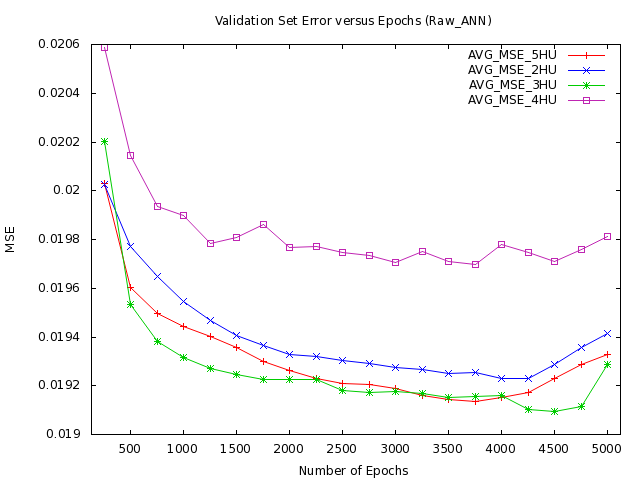
\includegraphics[scale=0.50]{raw_ann_validation_error_epochs}
		\caption[Validation set error versus number of epochs for Raw\_ANN using fixed architecture]{Validation set error versus number of epochs for Raw\_ANN using a fixed architecture. The lower MSE is reached by using 3 hidden units and training for $4500$ epochs.}
		\label{fig:raw_ann_validation_error_epochs}
	\end{center}
\end{figure}
\begin{figure}[H]
	\begin{center}
		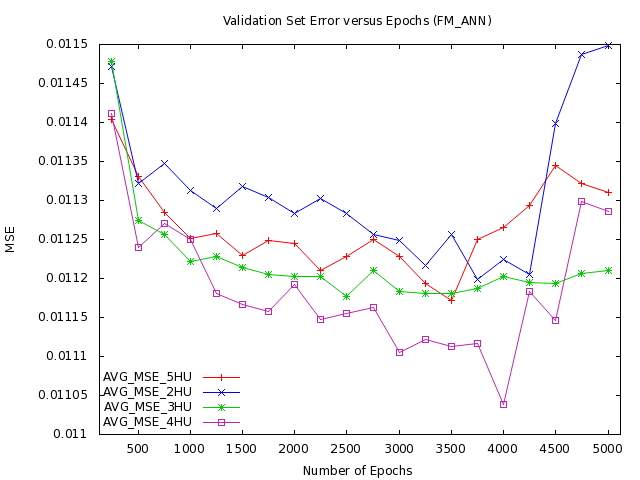
\includegraphics[scale=0.50]{fm_ann_validation_error_epochs}
		\caption[Validation set error versus number of epochs for FM\_ANN using fixed architecture]{Validation set error versus number of epochs for FM\_ANN using a fixed architecture. The lower MSE is reached by using 4 hidden units and training for $4000$ epochs.}
		\label{fig:fm_ann_validation_error_epochs}
	\end{center}
\end{figure}
\begin{figure}[H]
	\begin{center}
		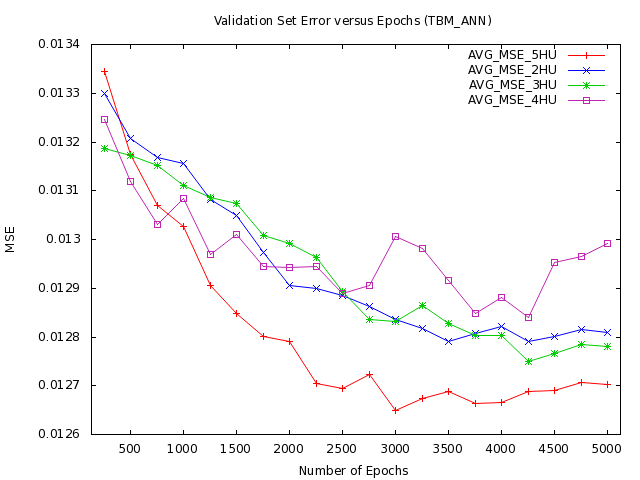
\includegraphics[scale=0.50]{tbm_ann_validation_error_epochs}
		\caption[Validation set error versus number of epochs for TBM\_ANN using fixed architecture]{Validation set error versus number of epochs for TBM\_ANN using a fixed architecture. The lower MSE is reached by using 5 hidden units and training for $3000$ epochs.}
		\label{fig:tbm_ann_validation_error_epochs}
	\end{center}
\end{figure}
\begin{figure}[H]
	\begin{center}
		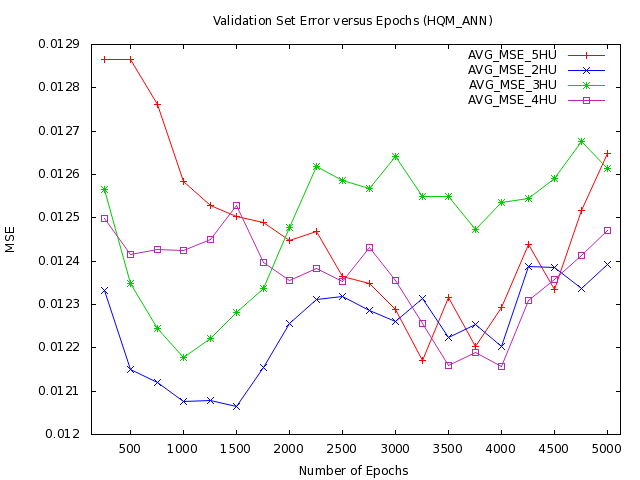
\includegraphics[scale=0.50]{hqm_ann_validation_error_epochs}
		\caption[Validation set error versus number of epochs for HQM\_ANN using fixed architecture]{Validation set error versus number of epochs for HQM\_ANN using a fixed architecture. The lower MSE is reached by using 2 hidden units and training for $1500$ epochs.}
		\label{fig:hqm_ann_validation_error_epochs}
	\end{center}
\end{figure}


\begin{figure}[H]
	\begin{center}
		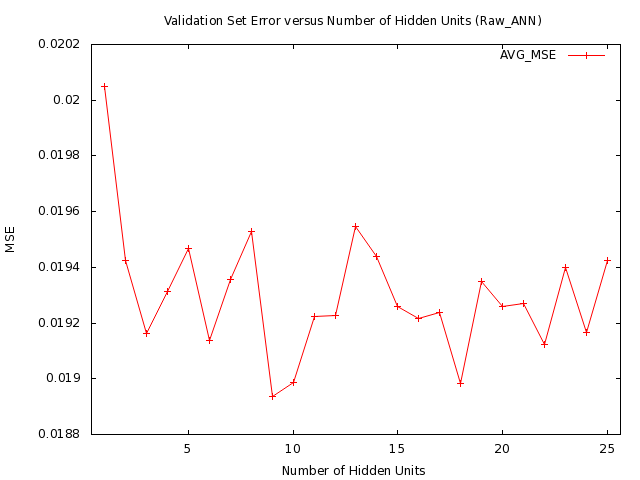
\includegraphics[scale=0.50]{raw_ann_validation_error_hu}
		\caption[Validation set error versus number of hidden units for Raw\_ANN using ca\-sca\-de-\-cor\-re\-la\-tion architecture]{Validation set error versus number of hidden units for Raw\_ANN using ca\-sca\-de-\-cor\-re\-la\-tion architecture. The lower MSE is reached by using 9 hidden units.}
		\label{fig:raw_ann_validation_error_hu}
	\end{center}
\end{figure}
\begin{figure}[H]
	\begin{center}
		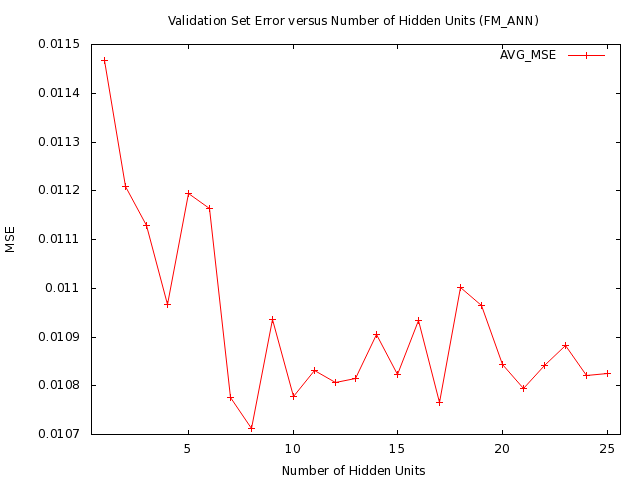
\includegraphics[scale=0.50]{fm_ann_validation_error_hu}
		\caption[Validation set error versus number of hidden units for FM\_ANN using ca\-sca\-de-\-cor\-re\-la\-tion architecture]{Validation set error versus number of hidden units for FM\_ANN using ca\-sca\-de-\-cor\-re\-la\-tion architecture. The lower MSE is reached by using 8 hidden units.}
		\label{fig:fm_ann_validation_error_hu}
	\end{center}
\end{figure}
\begin{figure}[H]
	\begin{center}
		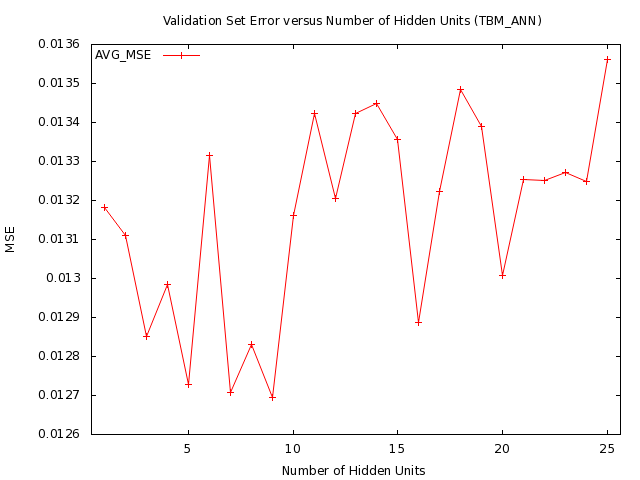
\includegraphics[scale=0.50]{tbm_ann_validation_error_hu}
		\caption[Validation set error versus number of hidden units for TBM\_ANN using ca\-sca\-de-\-cor\-re\-la\-tion architecture]{Validation set error versus number of hidden units for TBM\_ANN using ca\-sca\-de-\-cor\-re\-la\-tion architecture. The lower MSE is reached by using 8 hidden units.}
		\label{fig:tbm_ann_validation_error_hu}
	\end{center}
\end{figure}
\begin{figure}[H]
	\begin{center}
		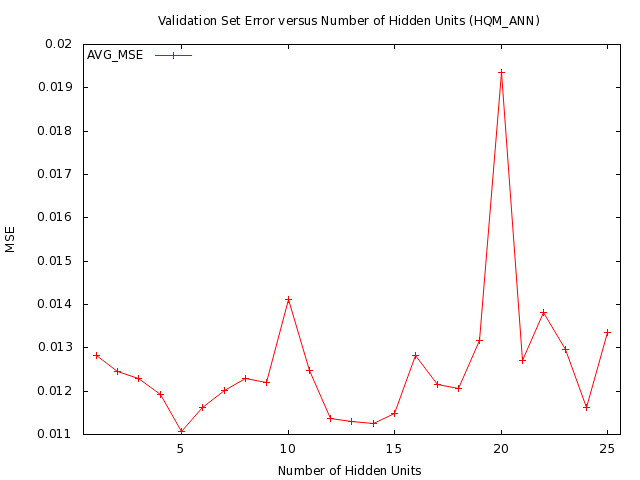
\includegraphics[scale=0.50]{hqm_ann_validation_error_hu}
		\caption[Validation set error versus number of hidden units for HQM\_ANN using ca\-sca\-de-\-cor\-re\-la\-tion architecture]{Validation set error versus number of hidden units for HQM\_ANN using ca\-sca\-de-\-cor\-re\-la\-tion architecture. The lower MSE is reached by using 5 hidden units.}
		\label{fig:hqm_ann_validation_error_hu}
	\end{center}
\end{figure}



\section{Clustering Optimizations}
\label{sec:clustering_optimization}

\subsection{Semi-Clustering Optimization}
\label{subsec:semiclustering_optimization}
In this section, the optimization of the best percentages for FM, TBM and HQM targets is provided by considering data from CASP-5, CASP-6 and CASP-7. These percentages serve to extract from all target models a subset of the best structures which will be used in the clustering procedure. \\
QMEAN is used in this optimization due to reduce problems related to overfitting. In fact, the QMEAN weight vector is optimized only on data from CASP-6. Being trained on the same data, the individual methods developed in this work obviously cannot be used in this procedure because they would provide an overestimation (see \S~\ref{subsec:training_and_testing_phases}). Discarding data from CASP-6, the final clustering accuracy substantially worsens using, as support MQAP, any implemented individual method or QMEAN itself. This fact could be explained with the lack of several models (in particular high quality models which are not frequent).\\
The optimization plots for FM, TBM and HQM targets are shown in Figures \ref{fig:thresholdFM} - \ref{fig:thresholdHQM} respectively. For FM targets, the best computed percentage is $93\%$ which achieves a Pearson correlation of $0.9036$. For TMB targets, the best percentage is $93\%$ obtaining $0.9617$ of Pearson correlation. Finally, for HQM targets, the best percentage is $85\%$ achieving a Pearson correlation of $0.9985$.
\begin{figure}[htbp]
	\begin{center}
		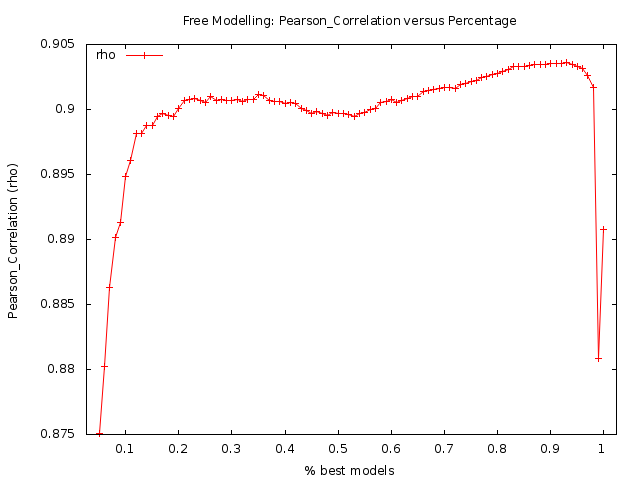
\includegraphics[scale=0.50]{thresholdFM}
		\caption[Optimization of the best percentage for FM targets]{Optimization of the best percentage for FM targets in CASP-5, CASP-6 and CASP-7. The highest Pearson correlation is $0.9036$, obtained by using $93\%$ of the best models.}
		\label{fig:thresholdFM}
	\end{center}
\end{figure}
\begin{figure}[htbp]
	\begin{center}
		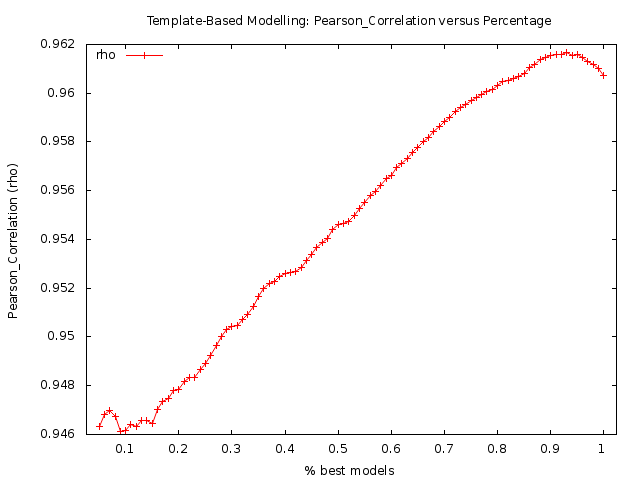
\includegraphics[scale=0.50]{thresholdTBM}
		\caption[Optimization of the best percentage for TBM targets]{Optimization of the best percentage for TBM targets in CASP-5, CASP-6 and CASP-7. The highest Pearson correlation is $0.9617$, obtained by using $93\%$ of the best models.}
		\label{fig:thresholdTBM}
	\end{center}
\end{figure}
\begin{figure}[htbp]
	\begin{center}
		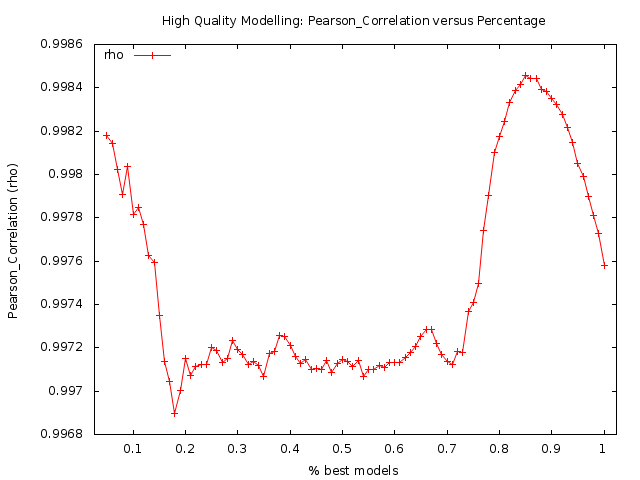
\includegraphics[scale=0.50]{thresholdHQM}
		\caption[Optimization of the best percentage for HQM targets]{Optimization of the best percentage for HQM targets in CASP-5, CASP-6 and CASP-7. The highest Pearson correlation is $0.9985$, obtained by using $85\%$ of the best models.}
		\label{fig:thresholdHQM}
	\end{center}
\end{figure}


\subsection{Parabolic Fraction Modelled}
\label{subsec:parabolic_fraction_modelled}
Table \ref{tab:fraction_modelled_functions} shows the improvement gained by using the $PFractionModelled$ feature with respect to the standard $FractionModelled$. The Pearson correlation is adopted in order to evaluate the performance of this optimization. Data from CASP-4 and CASP-8 are used as comparison. To illustrate the improvement, QMEAN is chosen as support MQAP to the implemented clustering-based method. On the other hand, usage of the developed individual methods in place of QMEAN, as support MQAP, has reported the same results and, for this reason, the latter are omitted. The $PFractionModelled$ represents a significative improvement with respect to the $FractionModelled$ of $\approx 0.5\%$ in CASP-8, reducing also the presence of false positives without penalizing HQM scores. In the same dataset the $PFractionModelled$ improves the clustering algorithm of $\approx 0.8\%$ with respect to the same algorithm which does not consider any $FractionModelled$-like function.
\begin{table}[H]
\center
\begin{tabular}{lcc}
\toprule                % or \hline
\textbf{QMEANclustZ}	&\textbf{CASP-4}	&\textbf{CASP-8}\\
\midrule                % or \hline
	No $FractionModelled$	&0.9408	&0.9392\\
	$FractionModelled$	&0.9468	&0.9420\\
	$PFractionModelled$	&0.9477	&0.9473\\
\bottomrule               % or \hline
\end{tabular}
\caption[Different fraction modelled evaluation]{Pearson correlation achieved in the CASP-4 and CASP-8 test sets by QMEANclustZ configured with different fraction modelled functions. QMEANclustZ with the $FractionModelled$ feature outperforms QMEANclustZ without the use of the feature. However the application of the pure $FractionModelled$ feature often reduces  too much model scores. QMEANclustZ with the $PFractionModelled$ feature outperforms significatively all the other variants proposed.}
\label{tab:fraction_modelled_functions}
\end{table}


\clearpage

\section{Performance on the CASP-4 and CASP-8 Datasets}
This section aims to illustrate the results achieved from the clustering-based and individual methods developed in this work. Results are presented and discussed by considering two different test sets: CASP-4 and CASP-8 (see \S~\ref{subsec:training_and_testing_phases}). The latter is more important because it contains more targets and is built by keeping in mind the aim of the MQAP category at CASP. Thus, the CASP-4 test set serves to confirm the reliability of the implemented methods. For each scheme, both Pearson and Spearman correlations are used with the intent to gain more reliable and accurate results. \\
For the CASP-8 test set, a comparison against the best $9$ MQAPs that participated to the CASP-8 experiment is presented. These methods are currently the best of the world. Scores computed by these MQAPs are retrieved from the CASP web page.\\
For the CASP-4 test set, only the QMEAN scores are reported as comparison against an external method because QMEAN is the only MQAP completely available in the laboratory where this work has been developed and no data is available from the CASP website.\\
The feature extracted from the program TAPscore is shown to decrease the accuracy of the method when used. The reason could be associated to the use of protein models instead of experimental structures. Although this feature is adopted only for HQM models, which are models very similar to the native structure, the TAPscore program often returns a score of $0$ for certain target models. This fact could mislead the HQM\_ANN prediction.\\
The following sections present and discuss the performance achieved on the CASP-4 and CASP-8 test sets.


\subsection{Performance on the CASP-4 Dataset}
\label{subsec:performance_on_the_casp4_dataset}
Tables \ref{tab:casp4} and \ref{tab:casp4_cascade} report the performances achieved by using fixed and ca\-sca\-de-\-cor\-re\-la\-tion ANN architectures, respectively. Methods are not directly comparable because the initial neural networks are different due to the different number of input units occuring among schemes. However, by considering both Pearson and Spearman correlations a higher reliability and accuracy of methods could be achieved. The schemes \emph{std\_median} and \emph{std\_H\_median} report more reliable and higher accuracy results with respect to the other schemes. Figure \ref{fig:casp4_qmean} reports the QMEAN versus GDT\_TS scatter plot. Figure \ref{fig:casp4_qmeanclustZ} shows the accuracy of the clustering implemented in this work using QMEAN as support MQAP. Figures \ref{fig:casp4_std_H_medianQMEANrannclustZ} - \ref{fig:casp4_std_medianQMEANeannZ} illustrate the best scatter plots achieved by methods based on fixed ANN architectures. Figures \ref{fig:casp4_cascade_std_H_medianQMEANeannclustZ} - \ref{fig:casp4_cascade_std_medianQMEANrannclustZ} show the best scatter plots obtained by methods based on ca\-sca\-de-\-cor\-re\-la\-tion ANN architectures. \\
For fixed topology ANNs, the scheme \emph{std\_H\_median} substantially obtains the best correlations for both the individual and the clustering-based methods. The achieved best Pearson correlations are $0.8799$ and $0.9485$ for QMEANeannZ (scheme \emph{std\_median}) and QMEANeannclustZ (scheme \emph{std\_H\_median}) respectively. The gained best Spearman correlations are $0.7278$ and $0.9513$ for QMEANrannZ (scheme \emph{std\_H\_median}) and QMEANrannclustZ (scheme \emph{std\_H\_median}) respectively.\\
For ca\-sca\-de-\-cor\-re\-la\-tion ANNs, the best results are more accurate than those achieved using fixed topology ANNs. The best schemes are \emph{std\_median} and \emph{std\_H\_median}. QMEANeannZ (scheme \emph{std\_median}) and QMEANeannclustZ (scheme \emph{std\_H\_median}) achieve the best Pearson correlations of $0.8901$ and $0.9489$ respectively. On the other hand, QMEANeannZ (scheme \emph{std\_H\_median}) and QMEANrannclustZ (scheme \emph{std\_median}) gain the best Spearman correlations of $0.7601$ and $0.9515$ respectively. 
For both the architectures, almost all proposed individual methods outperform significatively QMEAN which achieves $0.7844$ and $0.7102$ of Pearson and Spearman correlations respectively.


\begin{table}[htbp]
\center
\begin{tabular}{lcc}
\toprule                % or \hline
\textbf{Method Variants} & \textbf{Pearson} & \textbf{Spearman} \\
	\midrule                % or \hline
	\emph{\textbf{std\_median}} & &\\
	QMEANrannZ	&0.8264	&0.7126\\
	QMEANeannZ	&\textbf{0.8799}	&0.7060\\
	QMEANrannclustZ	&0.9461	&0.9499\\
	QMEANeannclustZ	&0.9479	&0.9493\\
	\midrule                % or \hline	
	\emph{\textbf{std\_G\_median}}	 & &\\
	QMEANrannZ	&0.8448	&0.7262\\
	QMEANeannZ	&0.7664	&0.6681\\
	QMEANrannclustZ	&0.9468	&0.9504\\
	QMEANeannclustZ	&0.9471	&0.9467\\
	\midrule                % or \hline	
	\emph{\textbf{std\_H\_median}}	& &\\
	QMEANrannZ	&0.8346	&\textbf{0.7278}\\
	QMEANeannZ	&0.8798	&0.7237\\
	QMEANrannclustZ	&0.9463	&\textbf{0.9513}\\
	QMEANeannclustZ	&\textbf{0.9485}	&0.9499\\	
	\midrule                % or \hline	
	\emph{\textbf{std\_GH\_median}}	& &\\
	QMEANrannZ	&0.8340	&0.7102\\
	QMEANeannZ	&0.8390	&0.7061\\
	QMEANrannclustZ	&0.9456	&0.9498\\
	QMEANeannclustZ	&0.9471	&0.9473\\	
	\midrule                % or \hline	
	\emph{\textbf{std\_3n\_T\_median}}	& &\\
	QMEANeannZ	&0.8301	&0.7065\\
	QMEANeannclustZ	&0.9478	&0.9492\\	
	\midrule                % or \hline	
	\emph{\textbf{std\_3H\_HT\_median}}	& &\\
	QMEANeannZ	&0.8473	&0.7065\\
	QMEANeannclustZ	&0.9483	&0.9493\\		
	\midrule                % or \hline	
	\emph{\textbf{std\_3GH\_GHT\_median}}	& &\\
	QMEANeannZ	&0.8389	&0.7061\\
	QMEANeannclustZ	&0.9470	&0.9472\\
	\midrule                % or \hline
	\emph{\textbf{Clustering using QMEAN}} & &\\
	QMEANclustZ	&0.9477	&0.9448\\	
	\midrule                % or \hline	
	\emph{\textbf{External MQAPs}} & &\\	
	QMEAN	&0.7844	&0.7102\\
\bottomrule                % or \hline
\end{tabular}
\caption[Performance on the CASP-4 test set using neural networks based on fixed ANN architecture]{Correlation on the CASP-4 test set using neural networks based on fixed ANN architecture. The best results are shown in bold face (for Pearson and Spearman correlations, for individual and clustering-based methods). The scheme \emph{std\_H\_median} obtains the best correlation for both the individual and the clustering-based methods. All individual proposed methods outperform significatively QMEAN, except QMEANeannZ with Gauss integrals. All clustering-based methods that use ANNs as support MQAP show an improved Spearman correlation with respect to the same clustering that uses QMEAN as support MQAP.}
\label{tab:casp4}
\end{table}


\begin{table}[htbp]
\center
\begin{tabular}{lcc}
\toprule                % or \hline
\textbf{Method Variants} & \textbf{Pearson} & \textbf{Spearman} \\
	\midrule                % or \hline
	\emph{\textbf{std\_median}}	& & \\
	QMEANrannZ	&0.8364	&0.7189\\
 	QMEANeannZ	&\textbf{0.8901}	&0.7325\\
 	QMEANrannclustZ	&0.9469	&\textbf{0.9515}\\
 	QMEANeannclustZ	&0.9484	&0.9493\\
	\midrule                % or \hline
	\emph{\textbf{std\_G\_median}}	 & &\\
	QMEANrannZ	&0.8295	&0.6837\\
 	QMEANeannZ	&0.7997	&0.6567\\
 	QMEANrannclustZ	&0.9461	&0.9484\\
 	QMEANeannclustZ	&0.9450	&0.9437\\
	\midrule                % or \hline
	\emph{\textbf{std\_H\_median}} 	& &\\
	QMEANrannZ	&0.8341	&0.7433\\
 	QMEANeannZ	&0.8844	&\textbf{0.7601}\\
 	QMEANrannclustZ	&0.9471	&0.9505\\
 	QMEANeannclustZ	&\textbf{0.9489}	&0.9510\\
	\midrule                % or \hline
	\emph{\textbf{std\_GH\_median}}	& &\\
	QMEANrannZ	&0.7818	&0.6847\\
 	QMEANeannZ	&0.8270	&0.7149\\
 	QMEANrannclustZ	&0.9461	&0.9481\\
 	QMEANeannclustZ	&0.9470	&0.9491\\
	\midrule                % or \hline
	\emph{\textbf{std\_3n\_T\_median}}	& &\\
 	QMEANeannZ	&0.8300	&0.7313\\
 	QMEANeannclustZ	&0.9482	&0.9493\\
	\midrule                % or \hline	
	\emph{\textbf{std\_3H\_HT\_median}}	& &\\
	QMEANeannZ	&0.8343	&0.7072\\
	QMEANeannclustZ	&0.9486	&0.9499\\		
	\midrule                % or \hline
	\emph{\textbf{std\_3GH\_GHT\_median}}	& &\\
 	QMEANeannZ	&0.8290	&0.7166\\
 	QMEANeannclustZ	&0.9472	&0.9492\\
	\midrule                % or \hline
	\emph{\textbf{Clustering using QMEAN}} & &\\
	QMEANclustZ	&0.9477	&0.9448\\		
	\midrule                % or \hline
	\emph{\textbf{External MQAPs}}	& &\\
	QMEAN	&0.7844	&0.7102\\
\bottomrule                % or \hline
\end{tabular}
\caption[Performance on the CASP-4 test set using neural networks based on ca\-sca\-de-\-cor\-re\-la\-tion ANN architecture]{Correlation on the CASP-4 using neural networks based on ca\-sca\-de-\-cor\-re\-la\-tion ANN architecture. The best results are shown in bold face (for Pearson and Spearman correlations, for individual and clustering-based methods). By using the ca\-sca\-de-\-cor\-re\-la\-tion algorithm, the Spearman correlation is consistent with the growth of the Pearson correlation meaning results more reliable. The best results are also highter than those reported in the corrisponding Table \ref{tab:casp4}, which again could mean that the ca\-sca\-de-\-cor\-re\-la\-tion architecture is more accurate than the fixed one. Almost all proposed individual methods outperform significatively QMEAN. QMEANeannZ using Gauss integrals shows only a low increment of accuracy against QMEAN.}
\label{tab:casp4_cascade}
\end{table}


\begin{figure}[H]
	\begin{center}
		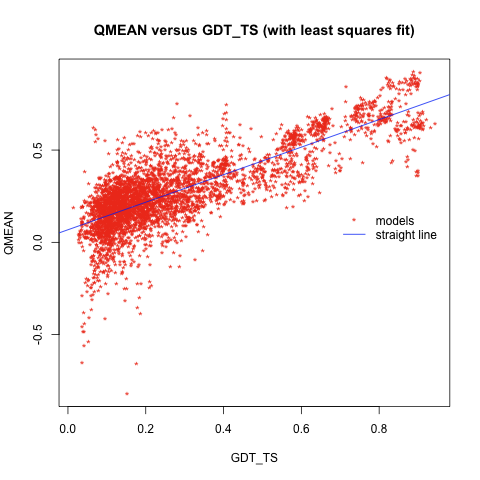
\includegraphics[scale=0.50]{casp4_QMEAN}
		\caption[QMEAN versus GDT\_TS on the CASP-4 test set]{QMEAN versus GDT\_TS on the CASP-4 test set. FM models on the left part of the scatter plot, that receive a negative score by QMEAN, represent obviously method errors.}
		\label{fig:casp4_qmean}
	\end{center}
\end{figure}

\begin{figure}[H]
	\begin{center}
		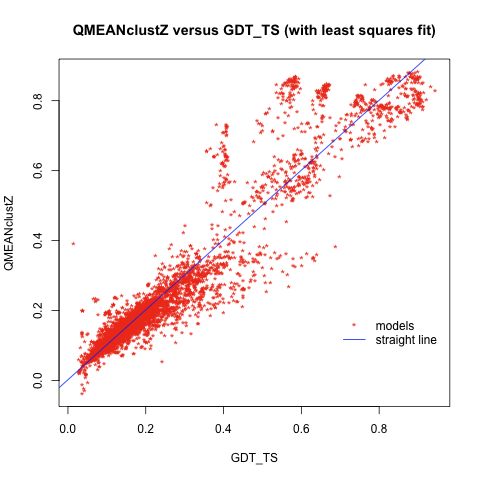
\includegraphics[scale=0.50]{casp4_QMEANclustZ}
		\caption[QMEANclustZ versus GDT\_TS on the CASP-4 test set]{QMEANclustZ versus GDT\_TS on the CASP-4 test set.}
		\label{fig:casp4_qmeanclustZ}
	\end{center}
\end{figure}

\begin{figure}[H]
	\begin{center}
		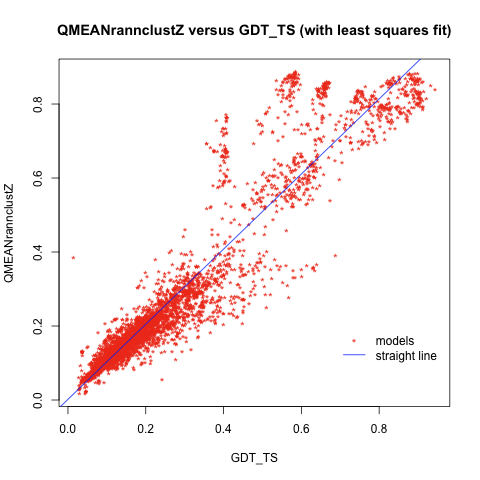
\includegraphics[scale=0.50]{casp4_std_H_medianQMEANrannclustZ}
		\caption[QMEANrannclustZ versus GDT\_TS on the CASP-4 test set, using hydrogen bonds and fixed ANN architecture]{QMEANrannclustZ versus GDT\_TS on the CASP-4 test set, using hydrogen bonds and fixed ANN architecture. A low improvement with respect to Figure \ref{fig:casp4_qmeanclustZ}  is visible on the left-down part of the scatter plot.}
		\label{fig:casp4_std_H_medianQMEANrannclustZ}
	\end{center}
\end{figure}

\begin{figure}[H]
	\begin{center}
		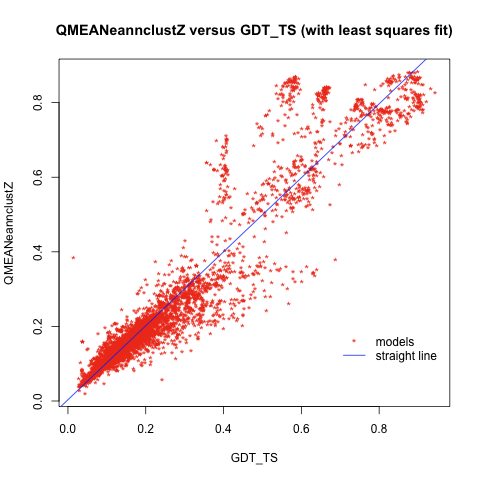
\includegraphics[scale=0.50]{casp4_std_H_medianQMEANeannclustZ}
		\caption[QMEANeannclustZ versus GDT\_TS on the CASP-4 test set, using hydrogen bonds and fixed ANN architectures]{QMEANeannclustZ versus GDT\_TS on the CASP-4 test set, using hydrogen bonds and fixed ANN architectures.}
		\label{fig:casp4_std_H_medianQMEANeannclustZ}
	\end{center}
\end{figure}

\begin{figure}[H]
	\begin{center}
		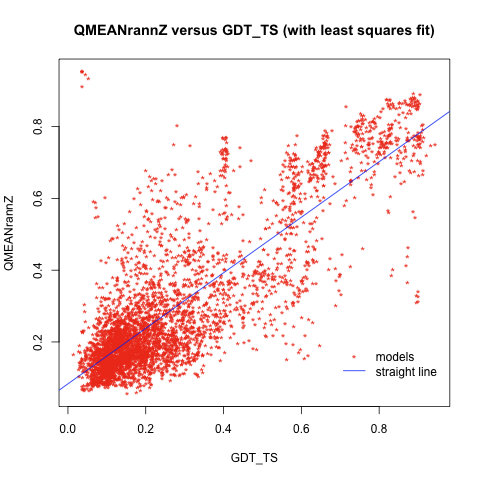
\includegraphics[scale=0.50]{casp4_std_medianQMEANrannZ}
		\caption[QMEANrannZ versus GDT\_TS on the CASP-4 test set, using fixed ANN architecture]{QMEANrannZ versus GDT\_TS on the CASP-4 test set, using fixed ANN architecture. FM scores are more grouped with respect to those given by QMEAN. However, the scatter plot still contains many false positives and negatives.}
		\label{fig:casp4_std_medianQMEANrannZ}
	\end{center}
\end{figure}

\begin{figure}[H]
	\begin{center}
		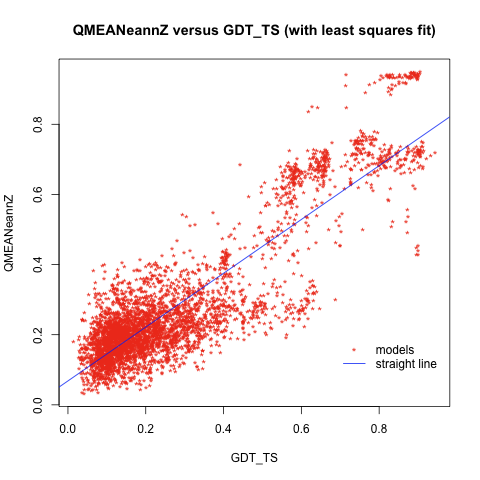
\includegraphics[scale=0.50]{casp4_std_medianQMEANeannZ}
		\caption[QMEANeannZ versus GDT\_TS on the CASP-4 test set, using fixed ANN architectures]{QMEANeannZ versus GDT\_TS on the CASP-4 test set, using fixed ANN architectures. Some false negatives are present on center-bottom of the scatter plot.}
		\label{fig:casp4_std_medianQMEANeannZ}
	\end{center}
\end{figure}

\begin{figure}[H]
	\begin{center}
		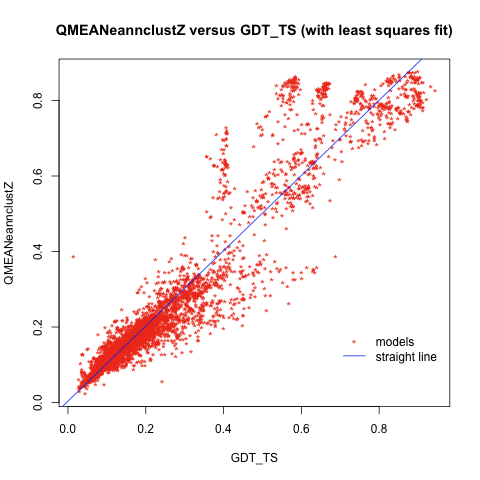
\includegraphics[scale=0.50]{casp4_cascade_std_H_medianQMEANeannclustZ}
		\caption[QMEANeannclustZ versus GDT\_TS on the CASP-4 test set, using hydrogen bonds and ca\-sca\-de-\-cor\-re\-la\-tion ANN architectures]{QMEANeannclustZ versus GDT\_TS on the CASP-4 test set, using hydrogen bonds and ca\-sca\-de-\-cor\-re\-la\-tion ANN architectures.}
	\label{fig:casp4_cascade_std_H_medianQMEANeannclustZ}
	\end{center}
\end{figure}

\begin{figure}[H]
	\begin{center}
		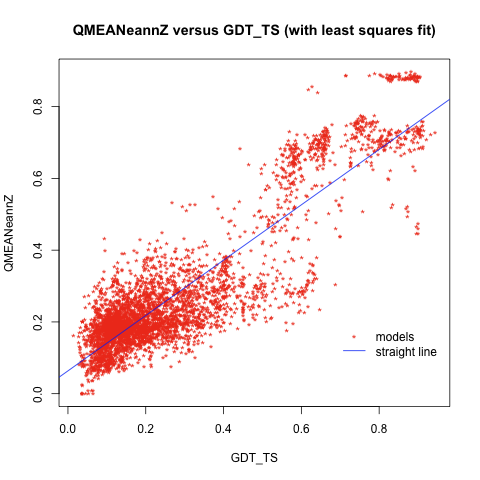
\includegraphics[scale=0.50]{casp4_cascade_std_medianQMEANeannZ}
		\caption[QMEANeannZ versus GDT\_TS on the CASP-4 test set, using ca\-sca\-de-\-cor\-re\-la\-tion ANN architectures]{QMEANeannZ versus GDT\_TS on the CASP-4 test set, using ca\-sca\-de-\-cor\-re\-la\-tion ANN architectures.}
	\label{fig:casp4_cascade_std_medianQMEANeannZ}
	\end{center}
\end{figure}

\begin{figure}[H]
	\begin{center}
		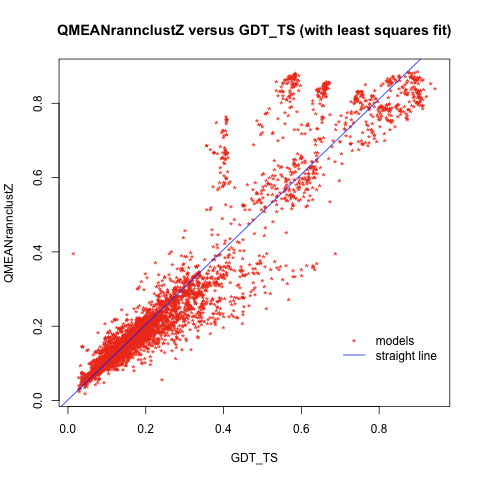
\includegraphics[scale=0.50]{casp4_cascade_std_medianQMEANrannclustZ}
		\caption[QMEANrannclustZ versus GDT\_TS on the CASP-4 test set, using ca\-sca\-de-\-cor\-re\-la\-tion ANN architecture]{QMEANrannclustZ versus GDT\_TS on the CASP-4 test set, using ca\-sca\-de-\-cor\-re\-la\-tion ANN architecture.}
\label{fig:casp4_cascade_std_medianQMEANrannclustZ}
	\end{center}
\end{figure}





\subsection{Performance on the CASP-8 Dataset}
\label{subsec:performance_on_the_casp8_dataset}
The CASP-8 test set is more relevant than the previous one because it contains more selected, difficult and recent protein targets. Tables \ref{tab:casp8} and \ref{tab:casp8_cascade} report the performance obtained respectively by using standard and cascading ANN architectures. The clustering-based methods implemented in this work, outperform significatively all other methods participating at the last CASP-8 experiment, held in December 2008. The best achieved Pearson and Spearman correlations are $0.9485$ and $0.9324$ respectively. The improvement with respect to ModFOLDclust, which is the best participating method and currently the best MQAP of the world, is of $\approx 1\%$ of global Pearson correlation. ModFOLDclust achieves $0.9395$ and $0.9210$ of Pearson and Spearman correlations respectively. All the five best methods achieve a Pearson correlation of $\approx 93\%$. Table \ref{tab:casp8_comparison} shows the comparison against the best $9$ methods plus QMEAN. Using Gauss integrals, methods do not perform well as confirmed in the previous test set, whereas the addition of hydrogen bonds improves the implemented method based solely on QMEAN features. In fact the best evaluated individual and clustering-based methods adopts the hydrogen bonds feature. QMEANclustZ represents an improvement with respect to QMEANclust showing that the clustering algorithm implemented in this work, outperforms the current one. The Pearson and Spearman correlations are $0.9473$ and $0.9309$ for QMEANclustZ, while QMEANclust obtains only $0.9317$ and $0.9199$ respectively. Figures \ref{fig:casp8_qmean} - \ref{fig:casp8_qmeanclustZ} illustrate the scatter plots of QMEAN, QMEANclust and the new QMEANclustZ. Figures \ref{fig:casp8_std_G_median_qmeaneannZ} - \ref{fig:casp8_std_median_qmeanrannZ} represent the most significative scatter plots by using fixed ANN architectures. Figures \ref{fig:casp8_cascade_std_median_qmeanrannZ} - \ref{fig:casp8_cascade_std_H_median_qmeaneannZ} depict the most important scatter plots using ca\-sca\-de-\-cor\-re\-la\-tion ANN architectures. Finally, Figures \ref{fig:casp8_modfoldclust}, \ref{fig:casp8_pcons_pcons} and \ref{fig:casp8_sam-t08-mqac} show the scatter plots of the three best methods participating in CASP-8. The best results are shown in bold face (for Pearson and Spearman correlations, for individual and clustering-based methods).\\
For fixed topology ANNs, the scheme \emph{std\_H\_median} obtains the best correlation for both the individual and the clustering-based methods. The achieved best Pearson correlations are $0.8177$ and $0.9485$ for QMEANeannZ (scheme \emph{std\_H\_median}) and QMEANrannclustZ (scheme \emph{std\_H\_median}) respectively. The gained best Spearman correlations are $0.8151$ and $0.9324$ for the same previously cited method variants respectively.\\
For ca\-sca\-de-\-cor\-re\-la\-tion ANNs, the best results are more accurate than those achieved using fixed topology ANNs. The best schemes are \emph{std\_median} and \emph{std\_H\_median}. QMEANeannZ (scheme \emph{std\_H\_median}) and QMEANrannclustZ (scheme \emph{std\_median}) achieve the best Pearson correlations of $0.8300$ and $0.9482$ respectively. The best Spearman correlations are $0.8237$ and $0.9321$ obtained by the same previously cited method variants respectively. 
For both the architectures, almost all proposed individual methods outperform significatively QMEAN which achieves $0.7651$ and $0.7655$ of Pearson and Spearman correlations respectively.



\begin{table}[htbp]
\center
\begin{tabular}{lcc}
\toprule                % or \hline
\textbf{Method Variants} & \textbf{Pearson} & \textbf{Spearman} \\
	\midrule                % or \hline
	\emph{\textbf{std\_median}}	& &\\
	QMEANrannZ	&0.7817	&0.7786\\
	QMEANeannZ	&0.7888	&0.7834\\
	QMEANrannclustZ	&0.9484	&0.9324\\
	QMEANeannclustZ	&0.9480	&0.9312\\
	\midrule                % or \hline	
	\emph{\textbf{std\_G\_median}} 	& &\\
	QMEANrannZ	&0.7750	&0.7826\\
	QMEANeannZ	&0.6671	&0.7386\\
	QMEANrannclustZ	&0.9436	&0.9277\\
	QMEANeannclustZ	&0.9431	&0.9275\\
	\midrule                % or \hline
	\emph{\textbf{std\_H\_median}} 	& &\\
	QMEANrannZ	&0.7879	&0.7886\\
	QMEANeannZ	&\textbf{0.8177}	&\textbf{0.8151}\\
	QMEANrannclustZ	&\textbf{0.9485}	&\textbf{0.9324}\\
	QMEANeannclustZ	&0.9484	&0.9318\\
	\midrule                % or \hline
	\emph{\textbf{std\_GH\_median}}	& & \\
	QMEANrannZ	&0.7595	&0.7674\\
	QMEANeannZ	&0.7517	&0.7736\\
	QMEANrannclustZ	&0.9438	&0.9280\\
	QMEANeannclustZ	&0.9431	&0.9269\\
	\midrule                % or \hline
	\emph{\textbf{std\_3n\_T\_median}}	& &\\
	QMEANeannZ	&0.7801	&0.7738\\
	QMEANeannclustZ	&0.9480	&0.9312\\	
	\midrule                % or \hline
	\emph{\textbf{std\_3H\_HT\_median}}	& &\\
	QMEANeannZ	&0.7981	&0.7863\\
	QMEANeannclustZ	&0.9484	&0.9304\\		
	\midrule                % or \hline
	\emph{\textbf{std\_3GH\_GHT\_median}}	& &\\
	QMEANeannZ	&0.7500	&0.7733\\
	QMEANeannclustZ	&0.9430	&0.9268\\
	\midrule                % or \hline
	\emph{\textbf{Clustering using QMEAN}} & &\\
	QMEANclustZ	&0.9473	&0.9309\\	
	\midrule                % or \hline
	\emph{\textbf{External MQAPs}} & &\\
	QMEAN	&0.7651	&0.7655\\
	QMEANclust	&0.9317	&0.9199\\
\bottomrule                % or \hline
\end{tabular}
\caption[Performance on the CASP-8 test set using neural networks based on fixed ANN architecture]{Correlation on the CASP-8 test set using neural networks based on fixed ANN architecture. The best results are shown in bold face (for Pearson and Spearman correlations, for individual and clustering-based methods). Both individual and clustering-based methods using hydrogen bonds achieve the best correlations. It suggests that hydrogen bonds represent a good new feature.}
\label{tab:casp8}
\end{table}


\begin{table}[htbp]
\center
\begin{tabular}{lcc}
\toprule                % or \hline
\textbf{Method Variants} & \textbf{Pearson} & \textbf{Spearman} \\
	\midrule                % or \hline
	\emph{\textbf{std\_median}}	& &\\
	QMEANrannZ	&0.7881	&0.7878\\
 	QMEANeannZ	&0.7932	&0.7908\\
 	QMEANrannclustZ	&\textbf{0.9482}	&\textbf{0.9321}\\
 	QMEANeannclustZ	&0.9480	&0.9314\\
	\midrule                % or \hline	
	\emph{\textbf{std\_G\_median}} 	& &\\
	QMEANrannZ	&0.7835	&0.7843\\
 	QMEANeannZ	&0.7170	&0.7776\\
 	QMEANrannclustZ	&0.9433	&0.9271\\
 	QMEANeannclustZ	&0.9431	&0.9274\\
	\midrule                % or \hline
	\emph{\textbf{std\_H\_median}} 	& &\\
	QMEANrannZ	&0.7948	&0.7949\\
 	QMEANeannZ	&\textbf{0.8300}	&\textbf{0.8237}\\
 	QMEANrannclustZ	&0.9480	&0.9317\\
 	QMEANeannclustZ	&0.9476	&0.9311\\
	\midrule                % or \hline
	\emph{\textbf{std\_GH\_median}}	& & \\
	QMEANrannZ	&0.7753	&0.7803\\
 	QMEANeannZ	&0.7195	&0.7512\\
 	QMEANrannclustZ	&0.9436	&0.9273\\
 	QMEANeannclustZ	&0.9424	&0.9268\\
	\midrule                % or \hline
	\emph{\textbf{std\_3n\_T\_median}}	& &\\
 	QMEANeannZ	&0.7925	&0.7900\\
 	QMEANeannclustZ	&0.9480	&0.9314\\
	\midrule                % or \hline
	\emph{\textbf{std\_3H\_HT\_median}}	& &\\
	QMEANeannZ	&0.8088	&0.8028\\
	QMEANeannclustZ	&0.9473	&0.9305\\		
	\midrule                % or \hline
	\emph{\textbf{std\_3GH\_GHT\_median}}	& &\\
 	QMEANeannZ	&0.7196	&0.7518\\
 	QMEANeannclustZ	&0.9423	&0.9268\\
	\midrule                % or \hline
	\emph{\textbf{Clustering using QMEAN}} & &\\
	QMEANclustZ	&0.9473	&0.9309\\		
	\midrule                % or \hline
	\emph{\textbf{External MQAPs}} & &\\
	QMEAN	&0.7651	&0.7655\\
	QMEANclust	&0.9317	&0.9199\\
\bottomrule                % or \hline
\end{tabular}
\caption[Performance on the CASP-8 test set by using neural networks based on ca\-sca\-de-\-cor\-re\-la\-tion ANN architecture]{Correlation on the CASP-8 test set using neural networks based on ca\-sca\-de-\-cor\-re\-la\-tion ANN architecture. The best results are shown in bold face (for Pearson and Spearman correlations, for individual and clustering-based methods). The scheme \emph{std\_H\_median} contains the best individual method proposed, whereas \emph{std\_median} presents the best clustering that uses as support MQAP, one based on ca\-sca\-de-\-cor\-re\-la\-tion ANN.}
\label{tab:casp8_cascade}
\end{table}



\begin{table}[htbp]
\center
\begin{tabular}{lcc}
\toprule                % or \hline
\textbf{MQAP Method} & \textbf{Pearson} & \textbf{Spearman} \\
	\midrule                % or \hline
	\emph{\textbf{Proposed methods}} &&\\
	QMEANrannZ (individual) &0.7948	&0.7949\\	
 	QMEANeannZ (individual) &0.8300 &0.8237\\
	QMEANrannclustZ (clustering-based) &0.9485	&0.9324\\	
	QMEANeannclustZ  (clustering-based) &0.9484	&0.9318\\	
	QMEANclustZ	&0.9473	&0.9309\\		
	\midrule                % or \hline
	\emph{\textbf{CASP-8 best methods}} &&\\	
 	ModFOLDclust	&0.9395	&0.9210\\
 	Pcons\_Pcons	&0.9375	&0.9243\\	
 	SAM-T08-MQAC	&0.9341	&0.9186\\
	QMEANclust	&0.9317	&0.9199\\
 	MULTICOM	&0.9312	&0.9145\\
 	McGuffin	&0.9275	&0.9075\\
 	MULTICOM-CLUSTER	&0.9133	&0.8928\\
 	selfQMEAN	&0.8977	&0.8892\\	
 	GS-MetalMQAPconsl	&0.8911	&0.8797\\
	\midrule                % or \hline
	\emph{\textbf{Basic method}} & &\\
	QMEAN	&0.7651	&0.7655\\
\bottomrule                % or \hline
\end{tabular}
\caption[Comparison of the best methods participating in CASP-8]{Comparison between methods developed in this work and the best methods participating in CASP-8, held in December 2008. The best methods are almost all clustering-based. QMEANrannZ and QMEANeannZ are obtained by using ca\-sca\-de-\-cor\-re\-la\-tion ANN architectures, whereas QMEANrannclustZ and QMEANeannclustZ are obtained by using fixed ANN architectures. The new proposed methods belong to the scheme \emph{std\_H\_median}. The implemented clustering-based methods (-clustZ) outperform all other methods and, in particular, they improve MoldFOLDclust, which is the best method of the world, of $\approx 1\%$ of Pearson correlation. Individual methods developed in this work significatively outperform QMEAN between $\approx 3\%$ and $\approx 6\%$ of Pearson correlation. Also, QMEANclustZ outperforms QMEANclust by $\approx 1.8\%$.}
\label{tab:casp8_comparison}
\end{table}


\begin{figure}[H]
	\begin{center}
		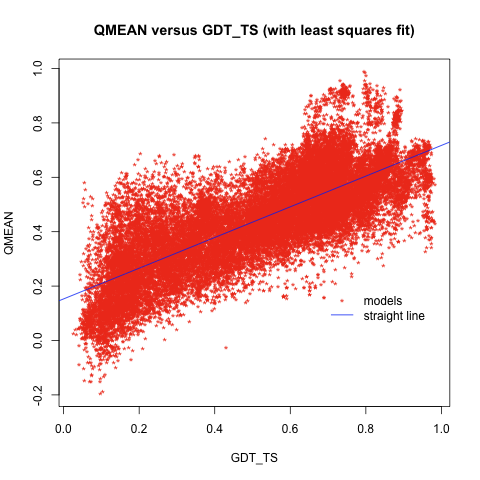
\includegraphics[scale=0.50]{casp8_QMEAN}
		\caption[QMEAN versus GDT\_TS on the CASP-8 test set]{QMEAN versus GDT\_TS on the CASP-8 test set. Globally, it presents the same accuracy for FM, TBM and HQM models.}
		\label{fig:casp8_qmean}
	\end{center}
\end{figure}

\begin{figure}[H]
	\begin{center}
		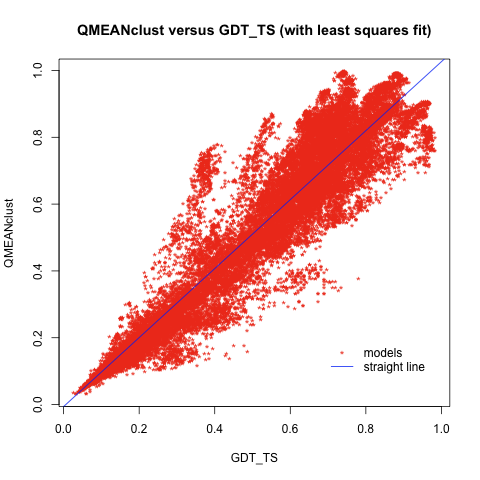
\includegraphics[scale=0.50]{casp8_QMEANclust}
		\caption[QMEANclust versus GDT\_TS on the CASP-8 test set]{QMEANclust versus GDT\_TS on the CASP-8 test set. It is the fourth best method concurring in CASP-8. It shows high accuracy for FM models, however does not assess exactly HQM model scores, leaving a hole in the high-right part of the scatter plot. Also many false positives and negatives are present in the center of the plot (TBM models).}
		\label{fig:casp8_qmeanclust}
	\end{center}
\end{figure}

\begin{figure}[H]
	\begin{center}
		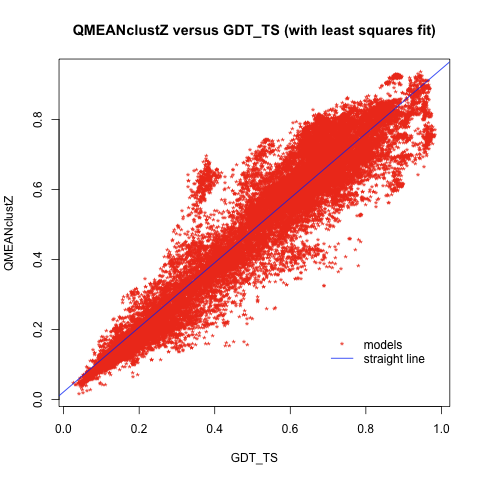
\includegraphics[scale=0.50]{casp8_QMEANclustZ}
		\caption[QMEANclustZ versus GDT\_TS on the CASP-8 test set]{QMEANclustZ versus GDT\_TS on the CASP-8 test set. This method improves QMEANclust by reducing the presence of false positives and negatives for TBM and HQM models. This plot cleanness is due to the presence of the feature $PFractionModelled$ that is able to lower incomplete model scores, but not so drastically as the pure $FractionModelled$ does. Also, it scores correctly HQM models.}
		\label{fig:casp8_qmeanclustZ}
	\end{center}
\end{figure}

\begin{figure}[H]
	\begin{center}
		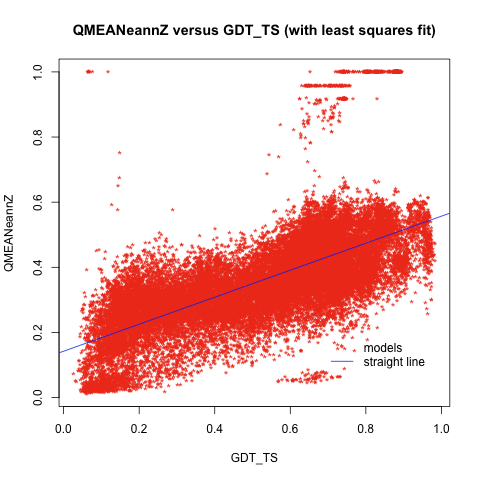
\includegraphics[scale=0.50]{casp8_std_G_medianQMEANeannZ}
		\caption[QMEANeannZ versus GDT\_TS on the CASP-8 test set, using Gauss integrals and fixed ANN architectures]{QMEANeannZ versus GDT\_TS on the CASP-8 test set, using Gauss integrals and fixed ANN architectures. This is the worst individual method. The predicted scores are very lower than the respective real scores, so the global Pearson correlation decreases with respect to that achieved by QMEAN. Methods using Gauss integrals are demonstrated to not be very reliable.}
		\label{fig:casp8_std_G_median_qmeaneannZ}
	\end{center}
\end{figure}

\begin{figure}[H]
	\begin{center}
		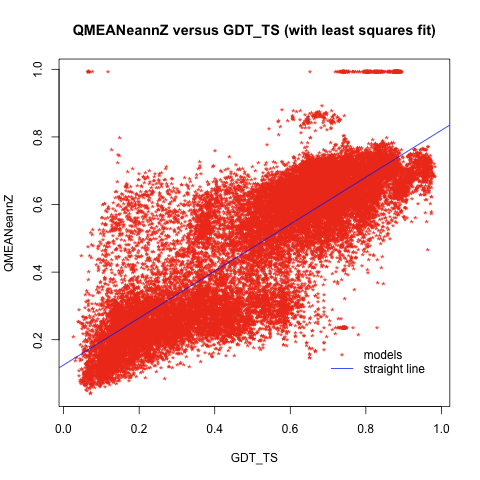
\includegraphics[scale=0.50]{casp8_std_H_medianQMEANeannZ}
		\caption[QMEANeannZ versus GDT\_TS on the CASP-8 test set, using hydrogen bonds and fixed ANN architectures]{QMEANeannZ versus GDT\_TS on the CASP-8 test set, using hydrogen bonds and fixed ANN architectures. A lot of false positives and negatives are present, however the two clouds are predicted correctly.}
		\label{fig:casp8_std_H_median_qmeaneannZ}
	\end{center}
\end{figure}

\begin{figure}[H]
	\begin{center}
		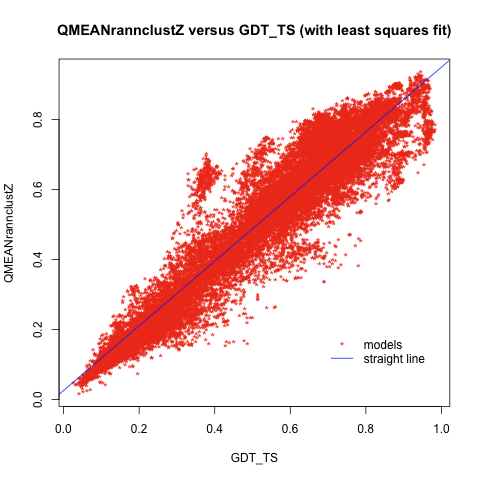
\includegraphics[scale=0.50]{casp8_std_H_medianQMEANrannclustZ}
		\caption[QMEANrannclustZ versus GDT\_TS on the CASP-8 test set, using hydrogen bonds and fixed ANN architecture]{QMEANrannclustZ versus GDT\_TS on the CASP-8 test set, using hydrogen bonds and fixed ANN architecture. This is the best clustering method presented with a Pearson correlation of $\approx 0.9485$. Only a little cloud of false positive is located in the center-left of the plot. Also HQM models are predicted correctly.}
		\label{fig:casp8_std_H_median_qmeanrannclustZ}
	\end{center}
\end{figure}

\begin{figure}[H]
	\begin{center}
		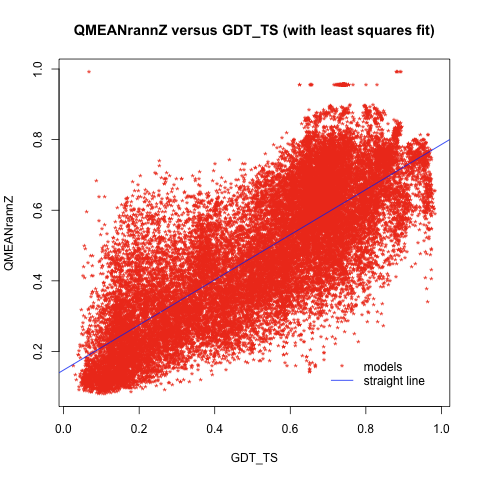
\includegraphics[scale=0.50]{casp8_std_medianQMEANrannZ}
		\caption[QMEANrannZ versus GDT\_TS on the CASP-8 test set using fixed ANN architecture]{QMEANrannZ versus GDT\_TS on the CASP-8 test set using fixed ANN architectures.}
		\label{fig:casp8_std_median_qmeanrannZ}
	\end{center}
\end{figure}

\begin{figure}[H]
	\begin{center}
		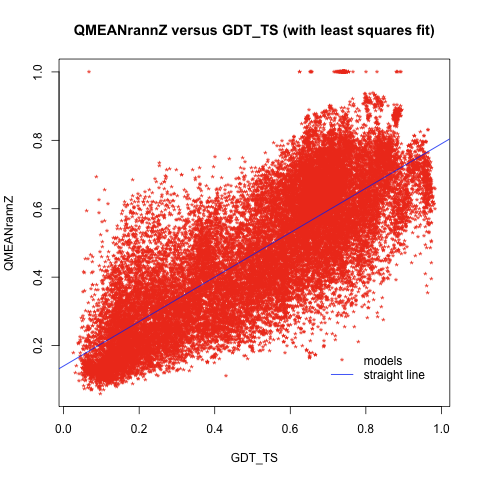
\includegraphics[scale=0.50]{casp8_cascade_std_medianQMEANrannZ}
		\caption[QMEANrannZ versus GDT\_TS on the CASP-8 test set, using ca\-sca\-de-\-cor\-re\-la\-tion ANN architecture]{QMEANrannZ versus GDT\_TS on the CASP-8 test set, using ca\-sca\-de-\-cor\-re\-la\-tion ANN architecture.}
		\label{fig:casp8_cascade_std_median_qmeanrannZ}
	\end{center}
\end{figure}

\begin{figure}[H]
	\begin{center}
		\includegraphics[scale=0.50]{casp8_cascade_std_medianQMEANrannclustZ}
		\caption[QMEANrannclustZ versus GDT\_TS on the CASP-8 test set, using ca\-sca\-de-\-cor\-re\-la\-tion ANN architecture]{QMEANrannclustZ versus GDT\_TS on the CASP-8 test set, using ca\-sca\-de-\-cor\-re\-la\-tion ANN architecture.}
		\label{fig:casp8_cascade_std_median_qmeanrannclustZ}
	\end{center}
\end{figure}

\begin{figure}[H]
	\begin{center}
		\includegraphics[scale=0.50]{casp8_cascade_std_H_medianQMEANeannZ}
		\caption[QMEANeannZ versus GDT\_TS on the CASP-8 test set, using hydrogen bonds and ca\-sca\-de-\-cor\-re\-la\-tion ANN architectures]{QMEANeannZ versus GDT\_TS on the CASP-8 test set, using hydrogen bonds and ca\-sca\-de-\-cor\-re\-la\-tion ANN architectures.}
		\label{fig:casp8_cascade_std_H_median_qmeaneannZ}
	\end{center}
\end{figure}

\begin{figure}[H]
	\begin{center}
		\includegraphics[scale=0.50]{casp8_ModFOLDclust}
		\caption[ModFOLDclust versus GDT\_TS on the CASP-8 test set]{ModFOLDclust versus GDT\_TS on the CASP-8 test set. This is the best method participating in CASP-8. The scatter plot present only some false negative. The cloud of false positive at coordinate $(0.4, 0.6)$ is common to all method predictions. That suggests a singular difficult target to predict.}
		\label{fig:casp8_modfoldclust}
	\end{center}
\end{figure}

\begin{figure}[H]
	\begin{center}
		\includegraphics[scale=0.50]{casp8_Pcons_Pcons}
		\caption[Pcons\_Pcons versus GDT\_TS on the CASP-8 test set]{Pcons\_Pcons versus GDT\_TS on the CASP-8 test set. This is the second best method participating in CASP-8. It presents many false negative and does not predict correctly any HQM models.}
		\label{fig:casp8_pcons_pcons}
	\end{center}
\end{figure}

\begin{figure}[H]
	\begin{center}
		\includegraphics[scale=0.50]{casp8_SAM-T08-MQAC}
		\caption[SAM-T08-MQAC versus GDT\_TS on the CASP-8 test set]{SAM-T08-MQAC versus GDT\_TS on the CASP-8 test set. This is the third best method participating in CASP-8. The correlation is linear and well formed. However there is not high accuracy for FM models}
		\label{fig:casp8_sam-t08-mqac}
	\end{center}
\end{figure}






\cleardoublepage

	
\chapter{Conclusions}
\label{conclusions}
In this work, two new individual methods (QMEAN\-rannZ and QMEAN\-eannZ) and three clustering-based methods (QMEAN\-clustZ, QMEAN\-rann\-clustZ and QMEAN\-eann\-clustZ) are developed. In order to assess the quality of models, the former two involve an approach based on neural networks. The distinction is made on the use of a single neural network to predict scores (-rannZ) or a neural network that is adopted only to categorize targets into three quality classes and, then, for each class, an expert neural network to assess scores of target models (-eannZ). Instead, the latter three methods evaluate model scores by taking into account a model ensemble and using a support method such as QMEAN, QMEAN\-rannZ and QMEAN\-eannZ in order to improve the accuracy. A new function, called parabolic fraction modelled, is used to reduce the scores of incomplete generated models. The benefit of this approach is to remove many false positives, avoiding to decrease too much the scores of partial models. Also, with the intention to understand and choose which other new features could be useful, three additional features that consider Gauss integrals, hydrogen bonds and TAP score, are investigated. Finally, the methods categorize targets before predicting model scores and this is shown to improve the accuracy. \\
The implemented individual methods are very fast. In fact, after having trained the neural network, the execution involves only information processing from input to output units. Although the training process requires several hours to complete, mainly due to the training set width and 5-fold cross validation, the running process only depends on the number of neural units that are used and this number is constant. On the other side, features from QMEAN, GIT, HBPLUS and TAP score can be computed once before applying neural network prediction. The algorithm used to cluster target models has a running time of $0(n^{2})$ where $n$ is the number of models proposed for a certain target. To improve the performance, similarity matrices can be computed once previously to the clustering process. \\
The developed clustering methods demonstrate high precision results for all target classes and in particular for the most important high quality models. Data from CASP-4 (40 targets for a total of 4,221 models) and CASP-8 (117 targets comprising 29,064 models) are used to test the proposed programs. The CASP-8 test set allows to compare the developed methods with the programs of other world-wide research teams that have participated to the last CASP experiment, held in December 2008. The individual methods implemented in this thesis, significatively outperform QMEAN between $\approx 3\%$ and $\approx 6\%$ of Pearson correlation. This fact demonstrates that non linear scoring functions that consider a set of features, perform better than linear ones for model quality assessment. The developed clustering-based methods (-clustZ) outperform all other methods participating in CASP-8. In detail, the improvement with respect to ModFOLDclust, which is the best participating method and currently the best MQAP in the world, is of $\approx 1\%$ of global correlation. The best achieved Pearson and Spearman correlations are $\approx 0.9485$ and $\approx 0.9324$ respectively. Also, QMEAN\-clustZ outperforms QMEAN\-clust by $\approx 1.8\%$. Results on the CASP-4 test set are consistent with those in CASP-8.\\
This work opens up many future directions. By selecting additional features besides those from QMEAN, hydrogen bonds are demonstrated to improve the method. This suggests that more investigation could be done in capturing and using these bonds and others, such as disulphide bonds, salt bonds, $\pi$-$\pi$ interactions, $\pi$-cation interactions and hydrophobic interactions, from proteins. The idea underlying Gauss integrals is interesting due to this characterization of proteins from a topological point of view. Using all $29$ descriptors computed by GIT is demonstrated in another work (see \cite{Bau2008}) to underperform with respect to the selection of a subset of them. However, it is possible that the inconsistency achieved by variants of the implemented methods that use Gauss integrals, is motivated by a bad selection of descriptors. Following this consideration, the worse performance achieved using all $29$ descriptors might be due to the great number of features which maybe reduces the importance of features extracted by other methods. A solution could be the definition of a supervised method, i.e. a neural network, that receives the $29$ Gauss invariants computed by GIT from a protein model and returns a single feature. This one would summarize the protein topology by condensing in itself all geometrical descriptors and avoiding to override the importance of other different features.\\
As expected, clustering-based methods significatively outperform individual ones. By weighting clustering scores with QMEAN\-rannZ with respect to QMEAN, performance improve. A interesting question might be the following: is clustering truly or does it tend to be a monotonic function? In other words, using a better support MQAP in order to weight clustering scores, does the performances improve? It would be interesting to use as support MQAP another clustering-based method, i.e. ModFOLDclust or Pcons\_Pcons. If the clustering function was or tended to be monotonic, then clustering scores would have been more accurate than those achieved in this work. Following this motivation, one could estimate the upper bound of the effectiveness reached by the implemented clustering. In fact, using the real GDT\_TS model scores instead of the predictions obtained by a support MQAP, the clustering scores should be the most accurate possible. Assuming the clustering to be a monotonic function, this study would lead to determine an upper bound in this clustering-based method.

\cleardoublepage


	
	
	
	% if using TeXShop
	% 1) In the menu line, choose Typeset > LaTeX or, equivalently, press <apple key>+T. You get the pdf file in a new window.
	% 2) Now choose Typeset > BibTeX. You see the console window with messages given by BibTeX.
	% 3) Go back to the tex or pdf windows and repeat 1).
	% 4) Repeat 1) again and you are done.
	% Every new change in the bib files should be followed by that cycle in order to include the modifications in the document.
	% Bibliography
	\clearpage
	\bibliography{biblio}
	\bibliographystyle{plain}
	\addcontentsline{toc}{chapter}{Bibliography}
	
	
	% Appendix
	\appendix
	


\chapter{Force Fields and Statistical Potentials}
\label{appendix:force_fields_statistical_potentials}
Many methods developed for model quality assessment use a particular optimization function, called scoring function, with the aim to summarize the most interesting features of a protein model.\\
Scoring functions used by MQAPs are similar to those defined in other fields of bioinformatics such as fold recognition, \emph{ab initio}, protein design, refinement of predicted three-\-di\-men\-sio\-nal protein structure, molecular mechanics or dynamics. Generally, energy functions are classified as follows:
\begin{itemize}
\item Force fields.
\item Statistical potentials.
\end{itemize}
A force field represents a predictive model described by using a physical approach, while a statistical potential builds a statistical model based on the amino acid distribution extracted from a set of known proteins. Generally, force fields are recognized to be more accurate than statistical potentials, although the latter approximate better the distance from the native protein structure (see Figure \ref{fig:energy_minimization}). The following sections examine the details of these categories.
\begin{figure}[tb]
	\begin{center}
		\includegraphics[scale=0.30]{energy_minimization}
		\caption[Example of energy minimization using force fields or statistical potentials]{Example of energy minimization using force fields or statistical potentials. The plot illustrates the differences between force fields and statistical potentials applications in the approximation of the real folding process of a hypothetic protein. Force fields (turquoise line) are more accurate than statistical potential (red line) in capturing the real energy of the protein structure (black line). However, statistical potentials approximate better the distance from the protein native structure that is located in the minimum energy point. A clear problem related to field forces is the presence of many local minima during the search in the conformational space.}
		\label{fig:energy_minimization}
	\end{center}
\end{figure}


\section{Force Fields}
\label{sec:force_fields}
Scoring functions based on force fields are heavily used in molecular mechanics or dynamics and protein design. The global energy of a certain protein conformation is estimated by a linear combination of different energy contributions. These are related to the short, medium and long-range interactions computed on all pairs of atoms that build the system.\\
Historically, this type of function was developed for two reasons:
\begin{description}
\item[Molecular mechanics.] Used to study small molecules as well as large biological systems or material assemblies with many thousands to millions of atoms. An application regards the optimization of three-\-di\-men\-sio\-nal protein structures, obtained experimentally or by a computational method. This is achieved by applying local improvement to the backbone and side chains, reducing collisions and minimizing the energy of the system.
\item[Molecular dynamics.] Simulations in which the target protein is surrounded by a huge number of water molecules, allowing it to evaluate all possible forces existing between atoms of the system. In this way, it is possible to study the movement of the structure in its real environment. 
\end{description}
A basic global energy of the structure is computed by using \emph{bonded terms} and \emph{non-bonded terms} as follows:
\begin{equation}
 	E = E_{bonded} + E_{non-bonded}
\end{equation}
where $E_{bonded}$ is defined as
\begin{equation}
 	E_{bonded} = E_{bond} + E_{angle} + E_{improper} + E_{torsion}
\end{equation}
and $E_{non-bonded}$ as
\begin{equation}
 	E_{non-bonded} = E_{electrostatic} + E_{vanderWaals}
\end{equation}
These contributions are estimated by mathematical functions that relate the force between two atoms to their relative positions. Figure \ref{fig:potential_energy} shows the terms from both graphical and mathematical points of view.\\
\begin{figure}[tb]
	\begin{center}
		\includegraphics[scale=0.40]{pe}
		\caption[Functions to describe energy terms]{Functions to describe energy terms. $E_{bond}$ and $E_{angle}$, called also bond stretching and angle bending respectively, are described by simple harmonic functions. Harmonic potentials are also used to represent the planarity of some groups. This kind of potential is known as improper dihedrals, $E_{improper}$. Torsion angles are represented by sinusoidal energies, $E_{torsion}.$ The electrostatic attraction or repulsion between two charges is described by Coulomb's law, $E_{electrostatic}$. The Lennard-Jones potential models the attractive and repulsive interactions, $E_{vanderWaals}$. (Source: \href{http://cmm.info.nih.gov/intro\_simulation/node15.html}{http://cmm.info.nih.gov/intro\_simulation/node15.html}).}
		\label{fig:potential_energy}
	\end{center}
\end{figure}
\emph{Bonded terms}, i.e. $E_{bond}$, $E_{angle}$ and $E_{torsion}$, are applied to a set of two to four atoms respectively, that are covalently bonded. The term $E_{improper}$ is used to describe the planarity of some groups, i.e. the amide planes of proteins. These terms describe structural constraints of the protein. The idea is that the larger is the distance between the measured and expected values, the more the scoring function penalizes the protein conformation.
$\emph{Non-bonded terms}$, i.e. $E_{electrostatic}$ and $E_{vanderWaals}$, deal with non covalent bonds between atoms. The former approximates the protein model using dielectric constants dependent on the distance of charged groups with the aim to estimate the Coloumb interactions. The latter studies the variation of the energy in function of the distance between atoms. It includes two components: strong short-ranged repulsive and weak long-ranged attractive. It is used with the intention to reduce structural overlaps. Typically, force fields are computed by considering only physical models and theoretical knowledge, and not based on experimental observation such as the Ramachandran plot. Also, they do not take into account solvation contribution and interactions based on hydrogen bonds.



\section{Statistical Potentials}
\label{sec:statistical_potentials}
Statistical potentials, also called knowledge-based potentials, represent statistical parameters derived from the analysis of a database containing characteristics of known proteins. The key concept underlying statistical potentials is that the information collected from a wide significative dataset should be able to capture empirically some physico-chemical aspects of the protein structure. For instance, by analyzing a huge set of known protein structures, it could be found that some particular amino acids are more involved in the formation of a specific structural pattern, i.e. $\alpha$-helix or a $\beta$-strand, than others. Therefore, if the structural pattern is found in an unknown protein structure, it is reasonable to associate it to the residues considered more involved.\\
Generally, the probabilities are determined by statistical examination of native contacts present in a database of structures represented in the PDB. According to the energy landscape view of protein folding, structures that closely resemble the native state will be distinguishably lower in free energy than those that are different from the native state. These probabilities are converted into pseudo-energies by using equations similar to the Boltzmann law:
\begin{equation}
 	E = -KT ln(\frac{P_{observed}}{P_{expected}})
\end{equation}
where $K$ is the Boltzmann constant, $T$ is the temperature, while $P_{observed}$ and $P_{expected}$ are the probability of an observed event with respect to an expected one \cite{Sippl1990aa, Sippl1996aa}.\\
Statistical potentials are extracted from sequence, structural or functional databases. From the first type of database, potentials are computed by analyzing multiple-alignments of homologous proteins. From the second category of database, many informations can be extracted. For instance, the probability that an amino acid is located in the core or on the surface of a protein (that means if an amino acid is more buried or exposed) could be obtained. Finally, from the latter type of database, an important information that can be extracted is the probability that a certain pattern is related to a specific function. Statistical potentials are used in many fields of bioinformatics related to protein structure prediction and model quality assessment. The scoring function is computed in order to estimate the similarity between native structure and predicted model. It is important to highlight that as with every knowledge-based approach, no new information is obtained and the reliability is strictly related to the dataset quality.


\cleardoublepage
	
\chapter{Gauss Integrals}
\label{appendix:gauss_integrals}
The protein backbone is a curve in space. One well-known measure of how two curves interact is the Gauss integral, also called Gauss invariant. The generalized Gauss integrals originate in integral formulas of Vassiliev knot invariants \cite{Bar-Natan1995} and give absolute measures of protein geometry. The integrals may be understood as crossing numbers and correlations along the backbone of crossing numbers. Two of the simplest structural measures are considered: the writhe and the average crossing number. The writhe, $Wr$, of a closed space curve, $\gamma$, may be computed by using the Gauss integral
\begin{equation}
 Wr(\gamma) = \frac{1}{4\pi}\iint_{\gamma \times \gamma \backslash D} \omega(t_1, t_2)dt_1dt_2
\end{equation}
where $\omega(t_1, t_2) = [\gamma\ '(t_1), \gamma(t_1) - \gamma(t_2), \gamma\ '(t_2)] / |\gamma(t_1) - \gamma(t_2)|^3$, $D$ is the diagonal of $\gamma \times \gamma$, and $[\gamma\ '(t_1), \gamma(t_1) - \gamma(t_2), \gamma\ '(t_2)]$ is the triple scalar product. As $\omega(t_1, t_2) = \omega(t_2, t_1)$, the writhe may be calculated as an integral over a 2-simplex, namely
\begin{equation}
 I_{(1,2)}(\gamma) = Wr(\gamma) = \frac{1}{2\pi}\iint_{0 < t_1 < t_2 < L} \omega(t_1, t_2)dt_1dt_2
\end{equation}
For a polygonal curve $\mu$, the definition of the writhe is
\begin{equation}
 I_{(1,2)}(\mu) = Wr(\mu) = \sum_{0 < i_1 < i_2 < N} W(i_1, i_2)
\end{equation}
where $N$ is the size of the protein, with 
\begin{equation}
 W(i_1, i_2) = \frac{1}{2\pi}\int_{i_1 = t_1}^{i_1 + 1} \int_{i_2 = t_2}^{i_2 + 1} w(t_1, t_2)dt_1dt_2
\end{equation}
where $W(i_1, i_2)$ is the contribution to writhe coming from the $i_1$th and the $i_2$th line segments, which equals the probability to see the $i_1$th and the $i_2$th line segments cross from an arbitrary direction, multiplied by the sign of this crossing, see Figure \ref{fig:sphere_gi}. 
\begin{figure}[tb]
	\begin{center}
		\includegraphics[scale=0.80]{sphere_gi}
		\caption[Gauss integrals and crossings]{On the unit sphere, the filled area corresponds to normals of planes in which the two projected line segments are seen to cross. The two line segments are seen to cross with a probability $|W|$ equal to the filled area divided by the area of the whole sphere when averaged over all directions in space. A positive crossing is seen ($W$ positive) whenever the line segment in the front is traversed upwards and the rear line segment is traversed from right to left or if both line segments are traversed in the opposite direction. Otherwise a negative crossing is seen ($W$ negative).}
		\label{fig:sphere_gi}
	\end{center}
\end{figure}
Geometrically, the writhe is the signed average number of crossings averaged over the observer's position located in all space directions. \\
The unsigned average number of crossings seen from all directions is known as the average crossing number and is defined as
\begin{equation}
 I_{|1,2|}(\mu) = \sum_{0 < i_1 < i_2 < N} |W(i_1, i_2)|
\end{equation}
A whole family of structural measures, defined over the second and third order Gauss invariants, e.g. 
\begin{equation}
 I_{|1,3|(2,4)}(\mu) = \sum_{\substack{0 < i_1 < i_2 \\ 
			     < i_3 < i_4 < N}} |W(i_1, i_3)|W(i_2, i_4)
\end{equation}
and
\begin{equation}
I_{(1,5)(2,4)(3,6)}(\mu) = \sum_{\substack{0 < i_1 < i_2 < i_3 \\ 
				< i_4 < i_5 < i_6 < N}} W(i_1, i_5)W(i_2, i_4)W(i_3, i_6)
\end{equation}
may be constructed by using writhe and average crossing number as the basic building blocks. The usefulness of the higher order invariants is that these can be able to distinguish curves which have the same writhe and average crossing number.\\
To understand better, a simple example is reported. Consider the axis of each tube in Figure \ref{fig:curves} to be given by a polygonal curve. 
\begin{figure}[tb]
	\begin{center}
		\includegraphics[scale=0.60]{curves}
		\caption[Two tubes with the signs of the crossings seen in this projection]{Two tubes with the signs of the crossings seen in this projection.}
		\label{fig:curves}
	\end{center}
\end{figure}
When the two tubes are pushed down to almost lie in the plane, the $W(i, j)$ in the formula tends either to $-1$, to $0$ or to $+1$. In fact, if the line segments $i$ and $j$ are seen to lie apart in the figure, then in the plane limit they will lie apart and in the same plane. The set of directions from which they are seen to cross will diverge to a set of two arcs with measure $0$ on the unit 2-sphere. That is, $W(i, j)$ tends to $0$. However, if the two line segments are seen to cross in the planar projection in which they are pushed into, then in the limit they are seen to cross from all direction on the unit 2-sphere. Hereby, $W(i, j)$, tends to $\pm1$ depending on the sign of the crossing. The writhe of the left tube in Figure \ref{fig:curves} is $I_{(1,2)}(W_{left}) \approx 3 \times (+1) + 2 \times (-1) = +1$ and that of the right tube is $I_{(1,2)}(W_{right}) \approx 2 \times (+1) + 3 \times (-1) = -1$, while the average crossing number is $\approx 5$ for both tubes due to ignoring the signs of crossings.


\cleardoublepage

\end{document}
